\chapter{Geometrie auf der Kugeloberfläche\label{chapter:kugel}}
\lhead{Geometrie auf der Kugeloberfläche}
\begin{refsection}
\chapterauthor{Melina Staub und Fabian Schmid}

\section{Einleitung}

Seit jeher fasziniert den Menschen die Fahrt zur See. Nicht grundlos ist die Seefahrt eine der wichtigsten und ältesten Tätigkeiten der Menschheit. Der innerliche Drang neue Weltmeere und unbekannte Gebiete zu entdecken, die Fahrt zur See zu erleichtern und erträglicher zu machen, trieben die Menschen an, die Schiffe dieser Welt immer weiter zu entwickeln.

Die Idee der Kugelform der Erde ist älter als man zu denken vermag. Bereits der Schüler des antiken griechischen Philosophen Platon - Aristoteles schrieb in seiner Schrift \textit{Über den Himmel} aus dem 4. Jahrhundert v. Chr. etliche Gründe welche für die Gestallt der Erde als Kugel sprechen:\\

\begin{compactitem}
      \item Sämtliche schweren Körper streben zum Mittelpunkt des Alls. Da sie dies von allen Seiten her gleichmässig tun und die Erde im Mittelpunkt des Alls steht, muss sie eine kugelrunde Gestalt annehmen. 
\item Bei von der Küste wegfahrende Schiffen wird der Rumpf vor den Segeln der Sicht verborgen. 
\item In südlichen Ländern erscheinen südliche Sternbilder höher über dem Horizont.
\item Der Erdschatten bei einer Mondfinsternis ist stets rund.
\end{compactitem}


Jedoch war um 1492 - der Zeit der Entdeckung Amerikas durch Christoph Kolumbus, die Idee der Erde in Kugelform noch sehr umstritten. Er erkannte anhand den Theorien und Erkenntnissen der alten Griechen, vor allem Aristoteles, das die Erde eine Kugel sein muss. \\
Doch mit seinem Vorschlag einen Seeweg über den Atlantik nach Indien zu finden und nicht wie üblich um Afrika zu segeln, stiess er beim beim portugiesischen König auf taube Ohren. Sein Plan Indien über eine Route nach Westen zu erreichen, widersprach dem gesunden Menschenverstand. Wäre die Erde wirklich eine Kugel und man befände sich auf der unteren Erdhalbkugel, würde man herunterfallen.\\
Doch auch der damals übliche Glaube an die Erde in Scheibenform brachte so einige Risiken mit sich. Was würde passieren, wenn die Flotte das Ende der Scheibe erreicht hatte? Würden sie über den Erdrand hinweggleiten und in den Abgrund stürzen?\\
Erst nach viel Überzeugungsarbeit durch Kolumbus, setzte er sich am Spanischen Hof durch und segelte über die Westliche Route über den Atlantik und entdeckte schlussendlich Amerika.

Der praktische und greifbare Beweis das die Erde eine Kugel ist, lieferte rund 30 Jahre später der Portugiese Fernando Magellan. Mit seiner Weltumsegelung und seiner Ankunft in den Philippinen, bewies er definitiv das die Erde eine Kugel ist.\\

Nun wollen wir uns die Frage stellen, wie die alten Seefahrer ohne GPS und jeglichen modernen Navigationssystemen auf hoher See wussten wo sie sich befanden und was haben die Sterne mit alldem zu tun? Reisen Sie mit uns zurück in eine Zeit mit Sextant, Kompass und Sternkarten. In die Zeit der Seefahrer und Entdecker.


\section{Gross- und Kleinkreise}

Eine Kugeloberfläche lässt sich in zwei verschiedene Kreisarten einteilen  Gross- und Kleinkreise. 
Wir betrachten als erstes die Grosskreise:

\subsection{Grosskreise}

\begin{definition}
Ein Grosskreis ist ein grösstmöglicher Kreis auf einer Kugeloberfläche. Sein Mittelpunkt fällt immer mit dem Mittelpunkt der Kugel zusammen und ein Schnitt auf dem Grosskreis teilt die Kugel in jedem Fall in zwei („gleich grosse“) Hälften.
\end{definition}

Es gibt unendlich viele Möglichkeiten eine Kugel in zwei gleich grosse Stücke zu zerschneiden, 
daher gibt es auch unendlich viele Grosskreise. Wenn wir die Grosskreise auf einer Kugel mit diesen auf der Erde beschreiben, sprechen wir von Längengraden. Der Äquator beschreibt ebenfalls einen Grosskreis und ist daher ein spezieller Breitengrad, zu den Breitengraden später mehr.
Ein Elementarer Bestandteil bilden die Grosskreise in der sphärischen Trigonometrie. Mithilfe der Schnittpunkte verschiedener Grosskreise, lässt sich ein sphärisches Dreieck bilden auf welchem sich die sphärische Trigonometrie anwenden lässt.

\begin{center}
        \includegraphics[width=0.3\textwidth]{kugel/Beispielbild.jpg}
    \captionof{figure}{Bild Grosskreise}
\end{center}

\subsection{Kleinkreise}

\begin{definition}
Unter Kleinkreis versteht man jene Kreise auf einer Kugeloberfläche, deren Ebenen nicht den Kugelmittelpunkt enthalten, davon ausgenommen ist der Äquator.
\end{definition}

Die Kleinkreise eignen sich im Gegensatz zu den Grosskreisen \textit{nicht} für die sphärische Trigonometrie. 
Sie werden lediglich zur Bestimmung der Messgrössen, Winkelabstände oder des Höhenwinkels eines Gestirns verwendet. 

Wenn wir die Kleinkreise auf die Erdoberfläche projizieren betrachten wir die Breitengrade.

\begin{center}
        \includegraphics[width=0.3\textwidth]{kugel/Beispielbild.jpg}
    \captionof{figure}{Bild Kleinkreise}
\end{center}

Für die Navigation sind die Breitengrade aber ebenso bedeutend wie die Längengrade, da man nur mit beiden in Kombination seine genaue Position bestimmen kann.

\section{Sphärische Dreiecke / Kugeldreieck}

Der Begriff Sphärisches Dreieck oder Kugeldreieck ist ein sehr weitläufiger Begriff. 
Dabei können wir den Begriff in drei für uns wesentliche Dreiecke unterteilen:\\

\begin{compactitem}
\item Allgemeine Kugeldreiecke
\item Kugelzweieck
\item Eulersche’Dreiecke
\end{compactitem}

\begin{center}
        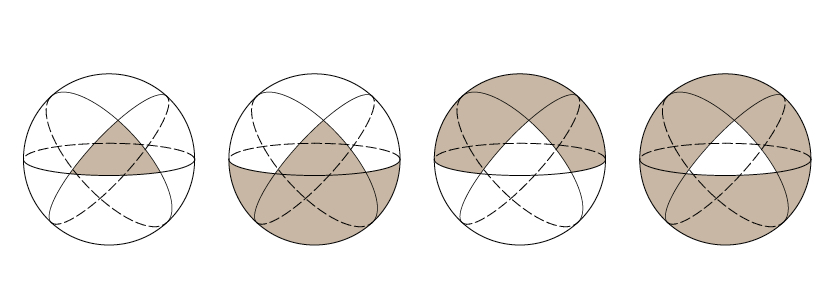
\includegraphics[width=0.9\textwidth]{kugel/Dreieckarten.jpg}
    \captionof{figure}{Dreiecksarten auf der Kugeloberfläche}
\end{center}

\subsection{Allgemeine Kugeldreiecke}

Ähnlich dem Dreieck in der Ebene hat das Dreieck auf der Kugel Seiten und Winkel. Allerdings werden die Seiten nicht in einer Länge angegeben sondern im Bogenmass. Auch hat das Dreieck auf der Kugel nicht zwingend $180^{\circ}$, die Winkelsumme liegt zwischen $180^{\circ}$ und zu $540^{\circ}$.

\subsection{Kugelzweieck}

Zwei Grosskreise auf der Kugeloberfläche zerlegen diese in vier gleich grosse Kugelzweiecke. 
Jedes dieser Dreieckseiten hat die Länge
$180^{\circ}$ oder $\pi$.
Der Flächeninhalt wird dabei nur durch den Winkel $\alpha$ zwischen den beiden Grosskreisen bestimmt.

\begin{center}
        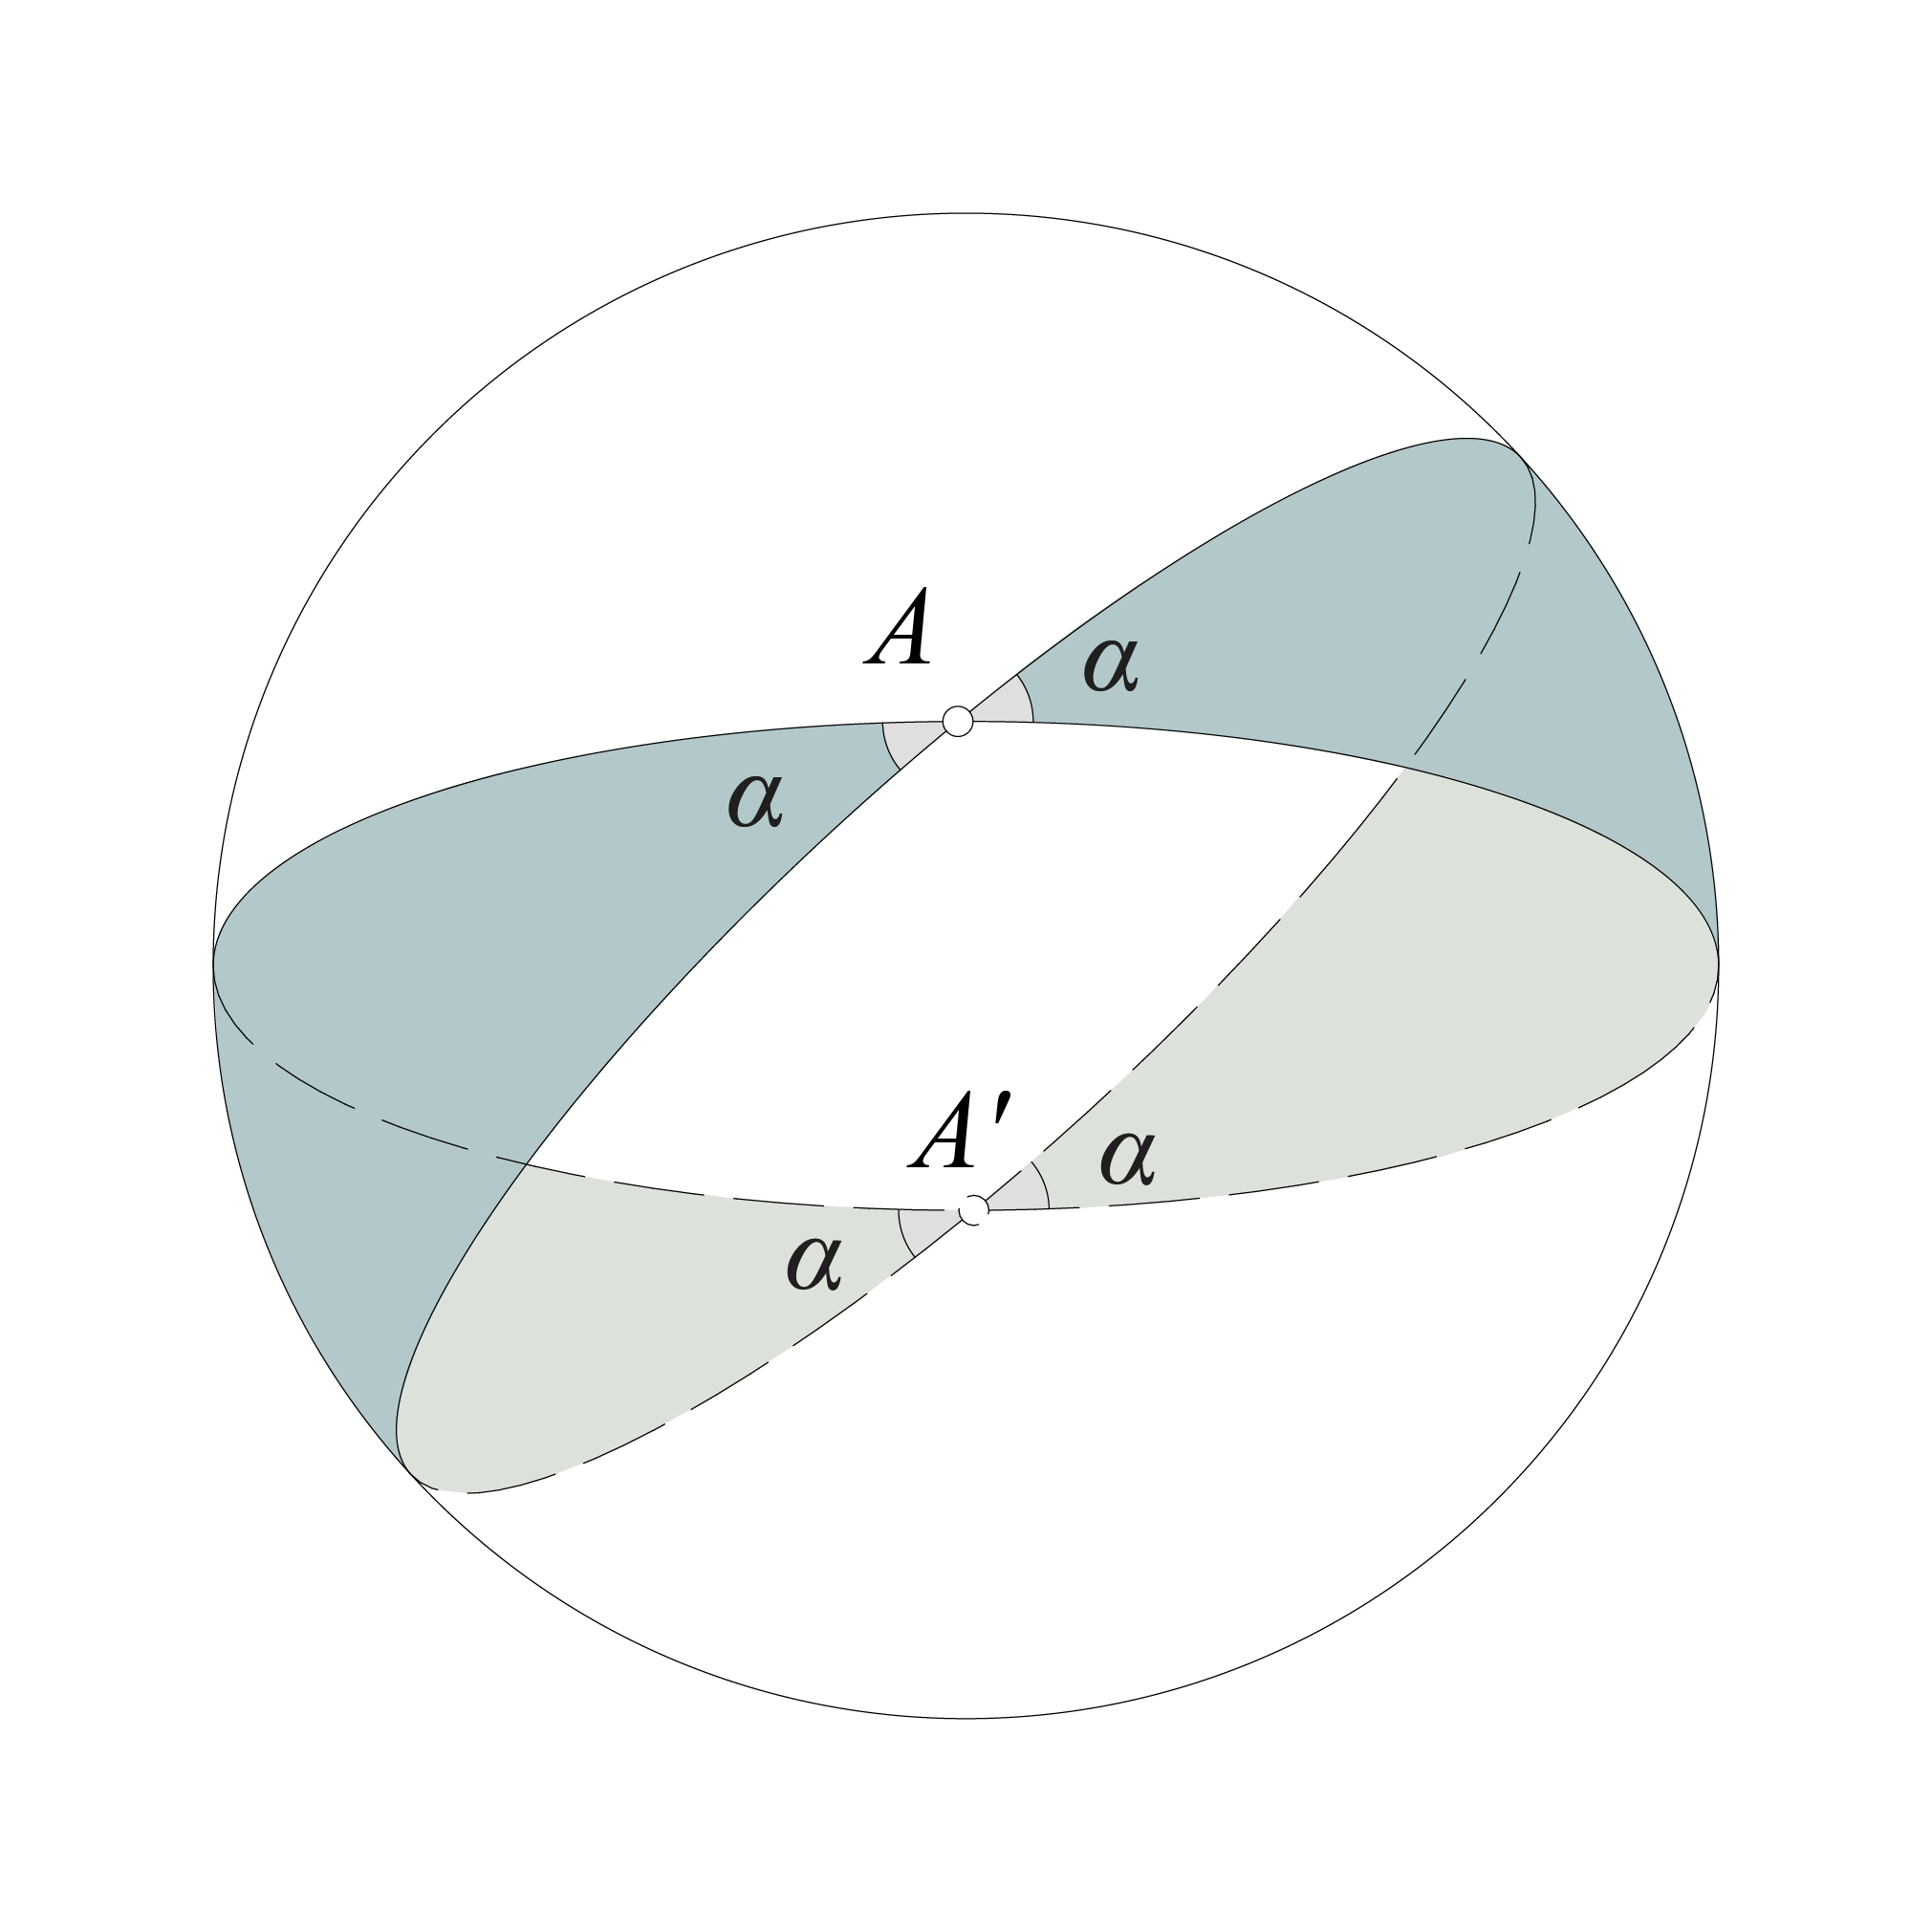
\includegraphics[width=0.3\textwidth]{kugel/Zweieck.jpg}
    \captionof{figure}{Bildung von Zweiecken durch Grosskreise}
\end{center}

Um den Flächeninhalt des Zweiecks zu erhalten, benötigen wir zuerst den Flächeninhalt der gesamten Kugel
\begin{align*}
A_{ Kugel } &= 4 \pi r^{2}
\end{align*}

Den Flächeninhalt der Kugel $A_{ Kugel }$ müssen wir noch mit dem Kugelsegment des Winkels $\alpha$ multiplizieren um dem Flächeninhalt des Zweiecks zu erhalten

\begin{equation}
A_{ Zweieck } = 4 \pi r^{2} \cdot \frac{ \alpha }{ 2 \pi }
\end{equation}

HIER NOCH EIN SATZ

\subsection{Eulersche’ Dreiecke}

Legt man drei Grosskreise auf eine Kugeloberfläche, bilden sich dabei acht Dreiecke. 
Ein solches Dreieck heisst Eulersches’Dreieck\footnote{%
Leonard Euler (1707-1783), berühmter Schweizer Mathematiker und Physiker. 
Nicht Eulersche’Dreiecke erhält man, indem man das Äussere des Dreieckes ABC betrachtet.}.
Diese Dreiecke werden weder durch die Verlängerung ihrer Seiten durchschnitten, 
noch haben sie Dreiecksseiten welche grösser als $180^{\circ}$ sind.

\begin{center}
        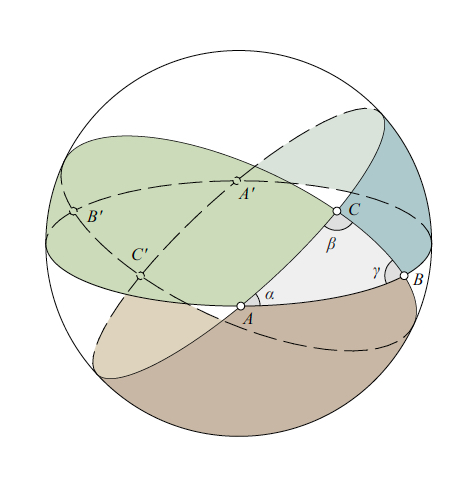
\includegraphics[width=0.4\textwidth]{kugel/Zweiecke.jpg}
    \captionof{figure}{Drei Grosskreise bilden ein sphärisches Dreieck}
\end{center}

In den nachstehenden Erklärungen und Herleitungen, sprechen wir ausschliesslich von Eulerschen’Dreiecken, da die umgeformten Winkelsätze der ebenen Trigonometrie nur auf diese Art von Kugeldreiecken angewendet werden kann.

$A_{ \overline{ ABC }}$ ist die Fläche des Dreieckes auf der Kugeloberfläche
In der ebenen Trigonometrie liegt die Winkelsumme eines Dreiecks bei
$180^{\circ}$.

Anders aber in der sphärischen Trigonometrie. Obschon sie einige Gemeinsamkeiten zur ebenen Trigonometrie aufweist, kann man nicht alles übernehmen.
So auch nicht wie Winkelsumme in einem sphärischen Dreieck.
Diese liegt bei:

\[
\begin{aligned}
\pi
&-
3\pi
&
&\text{\bigg \vert}
&
180^{\circ}
&-
540^{\circ}
\end{aligned}
\]

daraus lässt sich ableiten, das ein einzelner Winkel nicht grösser als $\pi$ oder $180^{\circ}$ sein darf. Ansonsten ist es kein Eulersches’Dreieck und wir dürfen die sphärische Trigonometrie nicht anwenden.\\
Wichtig anzumerken ist, dass die Seiten immer in Radiant beschrieben werden und nicht im Längenmass Meter wie wir es uns gewohnt sind. 
Bei den Dreiecksseiten handelt es sich um Kreisbögen und keine Strecken.

\section{Flächeninhalt sphärischer Dreiecke}

Der Flächeninhalt des Dreiecks $A_{ \triangle{ ABC }}$ berechnet sich aus den Winkeln $\alpha$, $\beta$, $\gamma$ und dem Kugelradius $r$ im Quadrat.
\begin{align*}
A_{ \triangle{ ABC }} &= (\alpha + \beta + \gamma) \cdot r^2
\end{align*}

\begin{center}
        \includegraphics[width=0.3\textwidth]{kugel/Beispielbild.jpg}
    \captionof{figure}{Bild FLäche dreieck}
\end{center}

Dies lässt sich folgendermassen herleiten: \\
Als erstes berechnen wir die Flächeninhalte der Zweiecke A, B und C

\begin{align*}
\text{Zweieck A}
&=
\triangle{ABC} + \triangle{A'BC} = 2 \alpha r^{ 2 } = A_{ \alpha }\\
\text{Zweieck B}
&=
\triangle{ABC} + \triangle{AB'C} = 2 \beta r^{ 2 } = A_{ \beta }\\
\text{Zweieck C}
&=
\triangle{ABC} + \triangle{ABC'} = 2 \gamma r^{ 2 } = A_{ \gamma }
\end{align*}

Addiert man nun die Flächeninhalte der einzelnen Zweiecke, ist diese Fläche gleich gross wie die der halben Kugel und zweimal des sphärischen Dreiecks $A_{ \triangle{ ABC }}$.

\begin{align*}
A_{ \alpha } + A_{ \beta } + A_{ \gamma } &= \frac{ 4\pi r^{ 2 } }{ 2 } + 2A_{ \triangle{ ABC }}
\end{align*}

Dies lässt sich umformen in

\begin{align*}
2\alpha r^{ 2 } + 2\beta r^{ 2 } + 2\gamma r^{ 2 } &= \frac{ 4\pi r^{ 2 } }{ 2 } + 2A_{ \triangle{ ABC }} \parallel:2
\end{align*}

Durch vereinfachen der Gleichung erhalten wir

\begin{align*}
\alpha r^{ 2 } + \beta r^{ 2 } + \gamma r^{ 2 } &= \pi r^{ 2 } + A_{ \triangle{ ABC }} \parallel-\pi r^{ 2 }\\
\end{align*}

Wir haben damit den folgenden Satz bewiesen:

\begin{satz}[\textit{Hallo ich heisse Flächeninhalt}]
\label{skript:kugel:satz:Flaecheninhalt}
\index{Flaecheninhalt}
\end{satz}

\begin{align*}
A_{ \triangle{ ABC }} &= r^{ 2 }\left(\alpha + \beta + \gamma - \pi\right) 
\end{align*}


\section{Sphärischer Exzess}
Anders als bei Dreiecken in der Ebene, ist die Winkelsumme bei sphärischen Dreiecken immer \textgreater \,  $\pi$.

\begin{align*}
\pi < \alpha + \beta + \gamma
\end{align*}

Der sphärische Exzess gibt dabei an, wie stark die Winkelsumme von $\pi$ abweicht.

\begin{align*}
\pi + \epsilon &= \alpha + \beta + \gamma \\
\end{align*}

Lösen wir nach $\epsilon$ auf:

\begin{equation}
\epsilon = \alpha + \beta + \gamma - \pi
\end{equation}

Zur Berechnung des Flächeninhalts eines sphärischen Dreiecks berechnet man demzufolge den sphärischen Exzess multipliziert mit dem Radius im Quadrat.
Dies zeigt, dass der Exzess direkt mit dem Flächeninhalt $A$ eines sphärischen Dreiecks zusammenhängt

\begin{align*}
\epsilon = \frac{A_{ \overline{ ABC }}}{r^2}
\end{align*}

\begin{center}
        \includegraphics[width=0.3\textwidth]{kugel/Beispielbild.jpg}
    \captionof{figure}{Bild Sphärischer Exzess}
\end{center}

Bei allgemeinen Kugeldreiecken gilt demnach:

\begin{align*}
\pi < \alpha + \beta + \gamma < 5\pi (900^{\circ})
\end{align*}


Bei Eulerschen’ Kugeldreiecken

\begin{align*}
\pi < \alpha + \beta + \gamma < 3\pi (540^{\circ})
\end{align*}

Der sphärische Exzess wird gleichmässig auf alle Winkel des Dreiecks aufgeteilt.

Bezieht man den sphärischen Exzess und die Formel des Flächeninhaltes auf die Erde und somit eine Kugel, kann man mit Hilfe eines beliebigen sphärischen Dreieckes und dessen Flächeninhalt auf den Radius der Kugel schliessen.

\subsection{Grenzfall - Satz von Legendre}

Würde der sphärische Exzess in der ebenen Trigonometrie angewendet, wäre dieser = 0.
Bei sehr kleinen sphärischen Dreiecken lässt sich dies annähernd wie in der ebenen Trigonometrie betrachten

\begin{quote} \textit{Ein kleines sphärisches Dreieck kann näherungsweise 
wie ein ebenes Dreieck mit denselben Seiten berechnet 
werden, wenn alle Winkel des ebenen Dreiecks die um 
je ein Drittel des sphärischen Exzesses verminderten 
Winkel des sphärischen Dreiecks nimmt.} \end{quote}
\begin{flushright} - Adrien-Marie Legendre (1752-1833), Paris 1787
\end{flushright}

Diese Aussage zeigt den Zusammenhang zwischen der 
Trigonometrie in der Ebene sowie in auf der Kugel
auf. Im speziellen bei sehr kleinen sphärischen 
Dreiecken ist die Winkelsumme nur unwesentlich 
grösser als $180^{\circ}$. 
Wichtig anzumerken ist, dass der Satz von Legendre 
für grosse, aber endliche Radien $r$ gilt.

\begin{center}
        \includegraphics[width=0.3\textwidth]{kugel/Beispielbild.jpg}
    \captionof{figure}{Bild Krümmung Gross und Klein}
\end{center}


\section{Sphärisch Analoge Winkelfunktionen}
Euklid von Alexandria\footnote{%
Euklid war ein griechischer Mathematiker. Er lebte wahrscheinlich 3 Jahrhunderte vor Christus. In seinem berühmtesten Werk \textit{Euklids Elemente} fasst er die Arithmetik und Geometrie seiner Zeit zusammen. \textit{Euklids Elemente} war 2000 Jahre lang als Lehrbuch in gebrauch und war bis Mitte des 19. Jahrhunderts nach der Bibel das weit verbreitetste Buch der Weltliteratur.}  beschrieb die Grundbegriffe der ebenen Geometrie mittels Punkt, Geraden, Ebene, Winkel und Dreieck. Ebendiese Dreiecke lassen sich mithilfe der ebenen Trigonometrie beschreiben. Dabei gelten die uns bekannten trigonometrischen Winkelfunktionen:\\

\text{Sinussatz:}
\begin{align*}
\frac{ a }{ sin(\alpha) } &= \frac{ b }{sin(\beta)} = \frac{ c }{ sin(\gamma) } = \frac{abc}{2A} = 2r\\
\end{align*}

\text{Cosinussatz:}
\begin{align*}
c^{ 2 } &= a^{ 2 } + b^{ 2 } - 2ab\cdot cos(\gamma)\\
b^{ 2 } &= a^{ 2 } + c^{ 2 } - 2ab\cdot cos(\beta)\\
a^{ 2 } &= b^{ 2 } + c^{ 2 } - 2ab\cdot cos(\alpha)
\end{align*}

Um diese Winkelfunktionen auf der Kugeloberfläche anwenden zu können, benötigen wir die sphärische Trigonometrie. Die oben beschriebenen Sätze lassen sich auf der Kugel nicht anwenden, sie werden aber als Grundlage und Gedankenstütze zur Herleitung der Sätze für das Kugeldreieck benötigt.

\subsection{Sphärischer Sinussatz}

\begin{center}
        \includegraphics[width=0.3\textwidth]{kugel/Beispielbild.jpg}
    \captionof{figure}{Bild Sinussatz}
\end{center}


Wir betrachten das folgende sphärische Dreieck auf einem Teilstück der Kugeloberfläche mit dem Radius $R= \overline{MA} = \overline{MB} = \overline{MC}$. Danach fügen wir ein ebenes Dreieck $\triangle=\overline{ADE}$ in das Kugelstück ein, welches den Eckpunkt $A$ des sphärischen Dreiecks beinhaltet und eine Abbildung des sphärischen Dreieckes bildet.

Es gilt

\begin{align*}
\overline{AD} &= R \cdot sin (c) \\
hA = \overline{AF} &= \overline{AD} \cdot sin(\beta) = R \cdot sin(c) \cdot sin(\beta)  
\end{align*}

Aus einer anderen Sichtweise kann man auch schreiben

\begin{align*}
h_{A} = R \cdot sin(b) \cdot sin(\gamma)  
\end{align*}

Durch gleichsetzen dieser Ausdrücke ergibt sich

\begin{align*}
R \cdot sin(c) \cdot sin(\beta) &= R \cdot sin(b) \cdot sin(\gamma) \\
\Rightarrow \quad \quad
sin(c) \cdot sin(\beta) &= sin(b) \cdot sin(\gamma) \\
\Rightarrow \quad \quad
\frac{sin (b)}{sin (c)} &= \frac{sin (\beta)}{sin (\gamma)}
\end{align*}

Analog dazu könnte man auch die Höhe $h_{B}$ nehmen und würde erhalten

\begin{align*}
sin(c) \cdot sin(\alpha) &= sin(a) \cdot sin(\gamma) \\
\Rightarrow \quad \quad
\frac{sin (a)}{sin (c)} &= \frac{sin (\alpha)}{sin (\gamma)}
\end{align*}

Aus diesen Erkenntnissen lässt sich der Sinussatz zusammenfassen

\begin{satz}[\textit{Der sphärische Sinussatz verhaltet sich wie der Sinus der Seiten wie der Sinus der Gegenwinkel, dies lässt sich beschreiben}]
\label{skript:kugel:satz:Sinussatz}
\index{Sinussatz}
\end{satz}

\begin{align*}
\sin(a) : \sin(b) : \sin(c) &= \sin(\alpha) : \sin(\beta) : \sin(\gamma) \\
 \\
\frac{sin(\alpha)}{sin(a)} &= \frac{sin(\beta)}{sin(b)} = \frac{sin(\gamma)}{sin(c)}
\end{align*} 


\subsection{Seitenkosinussatz}

Es sei das Stück einer Kugel mit dem sphärischen Dreieck $ABC$ und den Winkeln $\alpha, \beta, \gamma$ und den Seiten $a, b, c$. Die Senkrechten durch den Mittelpunkt, schneiden dabei die Eckpunkte des sphärischen Dreieckes. Wir erstellen in der Ebene ein Ähnliches Dreieck $A’B’C’$.

\begin{center}
        \includegraphics[width=0.3\textwidth]{kugel/Beispielbild.jpg}
    \captionof{figure}{Bild Seitenkosinus}
\end{center}

Dabei lassen sich die Strecken nach den uns bekannten Regeln der Trigonometrie beschreiben:

\begin{align*}
\overline{C'A'} &= d\cdot {tan(b)} \\
\overline{C'B'} &= d\cdot {tan(a)} \\
\overline{MA'} &= \frac{ d }{cos(b)} \\
\overline{MB'} &= \frac{ d }{cos(a)}
\end{align*} 

Dabei schreibt sich der Kosinussatz der Ebene wie folgt

\begin{align*}
c^{ 2 } &= a^{ 2 } + b^{ 2 } - 2ab \cdot cos(\gamma)
\end{align*}

Daher gilt für das Dreieck $A’B’C’$

\begin{align*}
\triangle \overline{A'B'}^{ 2 } &= \overline{ C'B' }^{ 2 } + \overline{ C'A' }^{ 2 } - 2 \cdot \overline{C'B'} \cdot \overline{ C'A' } \cdot cos(\gamma) \\
\Rightarrow \quad \quad
\triangle \overline{A'B'}^{ 2 } &= d^{ 2 } \cdot \left(\left(tan^{ 2 }(a) + tan^{ 2 }(b)\right) - 2\cdot tan(a) \cdot tan(b) \cdot cos(\gamma)\right)
\end{align*}


das gilt ebenso für das Dreieck $MA’B’$

\begin{align*}
\triangle \overline{ MA'B' }^{ 2 } &= \overline{ MB' }^{ 2 } + \overline{ MA' }^{ 2 } - 2\cdot \overline{ MB'} \cdot \overline{ MA' } \cdot cos(c) \\
\Rightarrow \quad \quad
\overline{ MA'B'}^{ 2 } &= \left(\frac{ d }{ cos(a) }  \right)^{ 2 } + \left(\frac{ d }{ cos(b)}  \right)^{ 2 } - 2 \cdot \frac{ d }{ cos(a)} \cdot \frac{ d }{ cos(b)} \cdot cos(c)
\end{align*}


Im Einheitskreis betrachtet ergibt dies

\begin{align*}
\overline{ MA'B' }^{ 2 } &= d^{ 2 } \cdot \left(\left(\frac{ 1 }{ cos(a) }  \right)^{ 2 } + \left(\frac{ 1 }{ cos(b) }  \right)^{ 2 } - 2 \cdot \frac{ 1 }{ cos(a)} \cdot \frac{ 1 }{ cos(b)} \cdot cos(c)\right)
\end{align*}


Durch berücksichtigen von $\frac{1}{\cos^{2}(x)}=\tan^{2}(x)+1$ folgt

\begin{align*}
\overline{ A'B'}^{ 2 } &= d^{ 2 } \cdot \left(\left(tan^{ 2 }(a) + tan^{ 2 }(b)\right) - 2 \cdot \frac{ 1 }{ cos(a)} \cdot \frac{ 1 }{ cos(b)} \cdot cos(c)\right) \\
\Rightarrow \quad \quad
\overline{ A'B'}^{ 2 } &= d^{ 2 } \cdot \left(\left(tan^{ 2 }(a) + 1\right) + \left(tan^{ 2 }(b) + 1\right) - \left(2 \cdot \frac{cos(c)}{cos(a) \cdot cos(b)}\right)\right)
\end{align*}


Durch gleichsetzen dieser beiden Ausdrücke folgt

\begin{align*}
2 \cdot tan(a) \cdot tan(b) \cdot cos(\gamma) &= -2+2 \cdot \frac{cos(c)}{cos(a) \cdot cos(b)}
\end{align*}

Durch umformen durch $\tan(a)=\frac{\sin(a)}{\cos(a)}$ und der Multiplikation mit  $\frac{1}{2}$ ergibt sich

\begin{align*}
\frac{\sin(a)}{\cos(a)} \cdot \frac{\sin(b)}{\cos(b)} \cdot \cos(\gamma) &= -1 + \frac{\cos(c)}{\cos(a) \cdot \cos(b)}
\end{align*}

Durch vereinfachen der Formel erhalten wir den Seitenkosinussatz der Seite $c$

\begin{align*}
\cos(a) \cdot \cos(b) + \sin(a) \cdot sin(b) \cdot \cos(\gamma) = \cos(c)
\end{align*}

Durch zyklische Vertauschung der Variablen erhält man den 

\begin{satz}[\textit{Im sphärischen Dreieck ist der Kosinus einer Seite gleich der Summe der Kosinusprodukte der beiden anderen Seiten und dem mit dem Kosinus des eingeschlossenen Winkels multiplizierten Sinusprodukt dieser Seiten}]
\label{skript:kugel:satz:Seitenkosinussatz}
\index{Seitenkosinussatz}
\end{satz}


\begin{align*}
{\cos a} &= {cos(b)} \cdot {cos(c)} + {sin(b)} \cdot {sin(c)} \cdot {cos(\alpha)}\\
{cos(b)} &= {cos(c)} \cdot {cos(a)} + {sin (c)} \cdot {sin(a)} \cdot {cos(\beta)}\\
{cos(c)} &= {cos(a)} \cdot {cos(b)} + {sin(a)} \cdot {sin(b)} \cdot {cos(\gamma)}\\
\end{align*}


ABSCHLUSSATZ

\subsection{Winkelkosinussatz}

Wenden wir den sphärischen Seitenkosinussatz auf dem Polardreieck an, erhalten wir
\begin{align*}
{\cos (a)} = {\cos (b)} \cdot {\cos (c)} + {\sin(b)} \cdot {\sin(c)} \cdot {\cos (\alpha)}
\end{align*}

\begin{center}
        \includegraphics[width=0.3\textwidth]{kugel/Beispielbild.jpg}
    \captionof{figure}{Bild Winkelkosinus/Polardreieck}
\end{center}

Durch die Beziehung zwischen dem Polardreieck und einem sphärischen Dreieck, können wir den Seitenkosinussatz folgendermassen umformen
\begin{align*}
{\cos (\pi-\alpha)} &= {\cos (\pi-\beta)} \cdot {\cos (\pi-\gamma)} + {\sin(\pi-\beta)} \cdot {\sin(\pi-\gamma)} \cdot {\cos (\pi-a)}
\end{align*}

Durch die Quadrantenbeziehung der trigonometrischen Funktionen im Einheitskreis folgt

\begin{align*}
\sin (\pi-\alpha) &= sin(\alpha)\\
\cos (\pi-\alpha) &= - cos (\alpha)\\
\end{align*}

Daher ergibt sich

\begin{align*}
{-\cos (\alpha)} &= {-\cos (\beta)} \cdot {-\cos (\gamma)} + {\sin(\beta)} \cdot {\sin(\gamma)} \cdot {-\cos (a)}
\end{align*}

Durch vertauschen der Vorzeichen erhalten wir den Winkelkosinussatz

\begin{satz}[\textit{Im sphärischen Dreieck ist der Kosinus eines Winkels gleich der Summe aus dem negativen Produkt der Kosinus der beiden anderen Winkel und dem mit dem Kosinus der gegenüberliegenden Seite multiplizierten Sinusprodukt der beiden anderen Winkel.}]
\label{skript:kugel:satz:Winkelkosinussatz}
\index{Winkelkosinussatz}
\end{satz}

\begin{align*}
{\cos (\alpha)} &= {-\cos(\beta)} \cdot {\cos(\gamma)} + {\sin (\beta)} \cdot {\sin(\gamma)} \cdot {\cos(a)}\\
{\cos (\beta)} &= {-\cos(\gamma)} \cdot {\cos(\alpha)} + {\sin (\gamma)} \cdot {\sin(\alpha)} \cdot {\cos(b)}\\
{\cos (\gamma)} &= {-\cos(\alpha)} \cdot {\cos(\beta)} + {\sin (\alpha)} \cdot {\sin(\beta)} \cdot {\cos(c)}\\
\end{align*}

ABSCHLUSSATZ

\section{Dualität auf der Kugel}

Durch die Herleitung des Winkelkosinussatzes haben wir zugleich die Dualität auf der Kugel bewiesen.

\begin{satz}[\textit{Die sphärische Geometrie ist eine projektive Geometrie. In der projektiven Geometrie lassen sich alle Sätze dualisieren, das heisst, die Begriffe Punkt und Geraden werden vertauscht; demzufolge auch Längen und Winkeln}]
\label{skript:kugel:satz:Dualitaet}
\index{Dualitaet}
\end{satz}

\begin{center}
        \includegraphics[width=0.3\textwidth]{kugel/Beispielbild.jpg}
    \captionof{figure}{Bild Dualität}
\end{center}

Dualisiert man nun als Beispiel einen Punkt und eine Gerade, bleibt die Beziehung zwischen dem Punkt und der Geraden erhalten.
Nimmt man nun den Punkt $A$ welcher auf der Geraden $b$ liegt, so verläuft die Duale Gerade $a$ durch den zur Geraden $b$ dualen Punkt $B$. 
Aber nicht nur die Beziehungen zwischen Punkten und Längen bleiben erhalten. Auch die Winkel und Längen gehen ineinander über wie wir es im Beweis des Winkelkosinussatzes gesehen haben.
Der Winkel $\gamma$ zwischen den beiden Seiten a und b entspricht auf der Einheitskugel dem Abstand zwischen den zu der Geraden dualen Punkten A und B.

\section{Navigation auf See}
Das besondere an Seekarten ist die Inhaltliche Ausrichtung. Anders wie Landkarten muss sie Informationen enthalten welche für den Kapitän und seine Besatzung von grosser Bedeutung sind. Vor allem in Küstennähe ist das navigieren eines Schiffes besonders gefährlich. So enthalten Seekarten etwas über Wassertiefen, Bodenbeschaffenheiten, Gezeiten, Küstenlinien, Landzungen und Windrichtungen.
Der Hauptunterschied dabei ist, das auf der Landkarte feste Positionen definiert und aufgezeigt werden, das einzige was sich verändert ist der Reisende selbst. Bei der Seekarte ist das anders, es werden veränderliche Einwirkungen der Natur festgehalten.

Dieser kleine Unterschied zeigt die Notwendigkeit auf, die Position und den Kurs seines Schiffes auf See immer ermitteln zu können.


\section{Geographische Koordinaten}

Nachdem klar war, das die Erde eine Kugel ist, wurde diese in ein Gradnetz aufgeteilt. Dabei wurden die Angaben für eine exakte Ortsbestimmung klar definiert und die bis heute gültigen Koordinaten bestimmt.
Dabei muss man sich nochmals in Erinnerung rufen, dass sich die Erde in 24h einmal um ihre eigene Achse dreht. Nach $360 ^{\circ}$ 
und somit einer vollen Umdrehung, steht sie wieder in ihrer Ursprungsposition und ein neuer Tag beginnt.

Die Koordinaten setzen sich aus folgenden Komponenten zusammen:

\[
\begin{aligned}
&\text{Grad } (^{\circ})
&
&\text{\bigg \vert}
&
&\text{Bogenminuten } (`)
&
&\text{\bigg \vert}
&
&\text{Bogensekunden } (``)
\end{aligned}
\]

Die Erdoberfläche wurde in je 360 Breiten- und Längengrade eingeteilt. Die Breitengrade haben zueinander einen Abstand von 111.31 km, dies entspricht auch dem Abstand der Längengrade am Äquator mit Zunehmender Nähe zu den Polen, nimmt dieser Abstand ab.

\[
\begin{aligned}
&1^{\circ}
&
&\text{\bigg \vert}
&
&4 \text{ Minuten}
&
&\text{\bigg \vert}
&
&111.31\text{ km}
\end{aligned}
\]

Berechnet man nun die Erdumdrehung von 360°, erhält man genau den Erdumfang am Äquator: \begin{align*} 40’074 \text{ km.}\end{align*}

Dabei geben die Bogenminuten und -sekunden dem Standort die gewünschte Exaktheit. Mit den vollständigen Koordinaten lässt sich der Standort auf einer Landkarte exakt bestimmen und einzeichnen.

\subsection{Erdachsenneigung}

Die Erdachse oder auch Rotationsachse der Erde ist um ca. $23.5^{\circ}$ geneigt.
Dadurch lassen sich Phänomene wie die vier Jahreszeiten sowie die unterschiedliche Längen der einzelnen Tage herleiten.
Für die nautische Navigation hat dies eine grosse Bedeutung, da je nach Neigung andere Sterne zu sehen sind, auch die Sonne ist an einem anderen Ort am Himmel zu finden.

\begin{center}
        \includegraphics[width=0.3\textwidth]{kugel/Beispielbild.jpg}
    \captionof{figure}{Bild Erdneigung}
\end{center}

Der Himmelsäquator ist die Linie, die orthogonal zur Sonne verläuft.
Die Ekliptil-Linie ist die Linie, die orthogonal zur Erdachse verläuft.
Der Schnittpunkt dieser Kreise wird als Frühlings- / Herbstpunkt bezeichnet und ist jeweils am 21. März / 21. Oktober des Jahres.
Der Frühlingspunkt $\Upsilon$ wird oft als Gestirnspunkt im nautischen Dreieck verwendet, genaueres wird im Kapitel zum nautischen Dreieck erklärt.


\subsection{Zeitzonen der Erde}
Wenn man nun die verschiedenen Zeitzonen der Erde betrachtet, macht die Verschiebung von jeweils einer Stunde durchaus Sinn, es lässt sich auf die Längengrade schliessen.
Zwischen den verschiedenen Zeitzonen liegen 15 Längengrade:
\begin{align*}
\text{15 Längengrade à 4 Minuten = 60 Minuten Zeitverschiebung = ca. 1665 km}
\end{align*}

Dabei ist die Zeitzone in welcher Mitte sich der Greenwich Meredian befindet die \textit{Greenwich Mean Time (GMT)} welche bis 1928 als Weltzeit galt. Im Jahr 1972 wurde diese umbenannt in die \textit{Coordinated Universal Time (UTC)} und wir von da an als Weltzeit $\pm$ 0.00 verwendet.


\section{Der Breitengrad}
Die Breitengrade bilden die bereits genannten Kleinkreise auf der Kugeloberfläche. Sie verlaufen in einem Abstand von genau 111 km parallel zum Äquator. Dabei stellt  dieser genau die Mitte zwischen Nord- und Südpol dar und teilt die Erdkugel in zwei gleiche Hälften. Somit wird von nördlicher und südlicher Breite gesprochen, je nach dem auf welcher Halbkugel man sich befindet.

\begin{center}
        \includegraphics[width=0.3\textwidth]{kugel/Beispielbild.jpg}
    \captionof{figure}{BILD SKIZZE DER GEOGRAFISCHEN BREITE ERDKUGEL}
\end{center}


\subsection{Geografische Breite $\phi$}
\begin{definition}
Die geografische Breite eines Standortes ist nichts anderes, als der Winkel am Erdmittelpunkt zwischen der Ebene des Äquators und der Geraden zum Standpunkt auf der Erdoberfläche.
\end{definition}

\begin{center}
        \includegraphics[width=0.3\textwidth]{kugel/Beispielbild.jpg}
    \captionof{figure}{Bild}
\end{center}


\subsection{Navigation mit den Breitengraden}
Da der Breitengrad bereits sehr früh ziemlich präzise bestimmt werden könnte, nutzten bereits die Seefahrer um Christoph Kolumbus den Breitengrad zur Navigation ihrer Flotten.
Den dieser lässt sich ziemlich einfach aus dem höchsten Sonnenstand oder einem Fixstern bestimmen. Dabei wird mit einem Jakobsstab\footnote{%
Der Jakobsstab ist ein früheres astronomisches Instrument zur Winkelmessung und wurde vor allem in der Seefahrt verwendet. Er ist in der Nautik der Vorläufer des Sextanten.} (später Sextant\footnote{%
Der Sextant ist ein nautisches Messinstrument zur Winkelmessung von Horizont und Fixstern (Gestirn)}) der Winkel zwischen dem Horizont und dem Fixstern gemessen. Der Winkel welchen man erhält, zieht man von 90° ab und erhält somit die geografische Breite. \\

\begin{center}
        \includegraphics[width=0.3\textwidth]{kugel/Beispielbild.jpg}
    \captionof{figure}{Bild}
\end{center}

Wenn man sich auf der Nordhalbkugel befindet, ist der Polarstern ein sehr guter Fixstern. Befindet sich ein Schiff nun sehr nahe am Nordpol, steht dieser nahezu senkrecht am Himmelszelt bei $90^{\circ}$. Würde es aber nahe dem Äquator stehen, erscheint dieser am Horizont bei $0^{\circ}$.

\subsection{Korrekturbeiwert}
Die Breitengrade auf der Erde haben nicht alle den selben Radius. Daher segelt man am Äquator viel länger dem Breitengrad entlang um zum nächsten Längengrad zu kommen wie in der nähe des Nord- oder Südpols.

\[
\begin{aligned}
&\text{1} (^{\circ})
&
&\text{\bigg \vert}
&
&\text{4 Minuten}
&
&\text{\bigg \vert}
&
&\text{111.13 km}
\end{aligned}
\]

\[
\begin{aligned}
&\text{0.25} (^{\circ})
&
&\text{\bigg \vert}
&
&\text{1 Minute}
&
&\text{\bigg \vert}
&
&\text{27.78 km}
\end{aligned}
\]

\[
\begin{aligned}
&\text{0.004166} (^{\circ})
&
&\text{\bigg \vert}
&
&\text{1 Sekunde}
&
&\text{\bigg \vert}
&
&\text{463m}
\end{aligned}
\]

Um die Minderung der Strecke zu erhalten, müssen wir den Cosinus des gemessenen Breitengrades berechnen und diesen mit der Abweichung auf dem Äquator von 1 Sekunde multiplizieren.

\begin{center}
        \includegraphics[width=0.3\textwidth]{kugel/Beispielbild.jpg}
    \captionof{figure}{Bild}
\end{center}

\[
\begin{aligned}
&\cos 90^\circ \cdot 463m = 463m
&
&\text{\bigg \vert}
&
&\cos 50^\circ \cdot 463m = 297.61m
&
&\text{\bigg \vert}
&
&\cos 0^\circ \cdot 463m = 0m
\end{aligned}
\]

Dies zeigt auf je näher man den Polen ist, desto weniger weit muss man Segeln um den nächsten Längengrad zu erreichen.

\section{Der Längengrad}
Die Längengrade bilden die bereits genannten Grosskreise auf der Kugeloberfläche.
Sie schneiden den Äquator im rechten Winkel, haben dort einen Abstand von 111 km zueinander und verbinden die Pole. Anders wie bei der geografischen Breite, ist in der Natur kein Längengrad gegeben welcher den Nullpunkt darstellt.

\begin{center}
        \includegraphics[width=0.3\textwidth]{kugel/Beispielbild.jpg}
    \captionof{figure}{Bild}
\end{center}


\subsection{Geografische Länge $\lambda$}
\begin{definition}
Die geografische Länge ist der Winkel an der Erdachse zum Nullmeridian.
\end{definition}

\subsection{Navigation mit den Längengraden}
Die geografische Länge lässt sich nicht so einfach bestimmen wie deren Breite. Für die Berechnung auf See benötigt man eine Referenzzeit eines Ortes mit bekannter Länge.
In der Zeit der Entdecker gab es noch keine mechanischen Uhren. Die Sonnenuhr war zudem ungeeignet, da diese nur die Uhrzeit am Standort mass und nicht die am Referenzort selbst. Die erste Pendeluhr wurde erst Mitte des 17. Jahrhunderts erfunden, was in der Schifffahrt aber auch nicht die Lösung brachte.\\
Pendeluhren auf einem Schiff sind ungeeignet, da das Pendel mit dem Wellengang aus dem Takt gebracht wird und somit die Uhr falsch geht.
Zu ungenau und gegen äussere Erschütterungen zu empfindlich waren später auch die federgetriebenen Uhren und die Unruh. Dazukamen die verschiedenen Klimazonen welche ein Schiff zu durchqueren hatten. Das Metall zog sich viel zu fest zusammen oder dehnte sich aus, was dazu führte das die Uhr unregelmässig lief.

Das sogenannte „Längenproblem“ stellte nicht nur bei der Navigation auf See ein Problem dar, es ergaben sich auch wirtschaftliche Konsequenzen. Die Schiffe mussten bis zur gewünschten geografischen Breite navigieren und segelten dann den Breitengrad entlang. Dabei waren die Schiffe oft Wochenlang unterwegs und segelten die „Breiten ab“ um an die gewünschte Position zu kommen. Dies führte zu erheblichen Zeitverlusten und viel längeren Reisezeiten.


\section{The Board of Longitude - Das Längenproblem}
Das Längenproblem beschäftigte alle grossen Seefahrernationen Europas. Die fehlenden Längengrade bei der Navigation führten zu vielen Schiffsunglücken. Dies zeigt auch die Dringlichkeit der Lösung dieses Problems auf: Nicht selten kam es vor, das sich auf den verloren gegangenen Schiffen Schätze in der Höhe von halben britischen Staatshaushalten befanden. Der Verlust solcher Schiffe war enorm.\\
Bereits um 1600 hatte der König von Spanien ein Preisgeld ausgeschrieben für denjenigen welcher eine Lösung für das Problem präsentieren konnte. Leider ohne Erfolg. \\

Nach einem tragischen Unglück im Jahr 1707 beidem der siegreiche Admiral Sir Cloudesley und seine 1’450 Mann sein Leben liessen, indem sie auf die Scilly-Inseln kurz vor Land’s End aufliefen und dabei die 21 Schiffe sanken, rückte das Problem wieder in den Vordergrund.
114 Jahre später, nach einer Petition von William Whiston und Humphry Ditton welche von Sir Isaac Newton und Edmond Halley untermauert wurde, reagierte das britische Parlament.
Es schrieb folgende Preisgelder für eine praktisch, brauchbare Lösung aus:\\

\begin{compactitem}
\item £ 20’000 - Abweichung von max. $\frac{1}{2}^{\circ}$
\item £ 15’000 - Abweichung von $\frac{2}{3}^{\circ}$
\item £ 10’000 - Abweichung von max. $1 ^{\circ}$
\end{compactitem}
\\
Im Kapitel der Korrekturbeiwertberechnung des Breitengrades haben wir erfahren, das eine Abweichung von $1 ^{\circ}$ am Äquator ca. 111km entsprechen - dies sind 60 Seemeilen.
Auf der Höhe des Ärmelkanals und damit London, beträgt die Abweichung nur noch 74km und somit 40 Seemeilen.//
Das Preisgeld entsprach einer enorm hohen Summe für diese Zeit. Der Kaufpreis für ein mittleres Schiff welches zur See fahren konnte lag bei etwa 1’500-2’500£, ein einzelner Arbeiter lebte mit 10£ im Jahr.
Würde man dieses Problem heute mit einer Abweichung von einem halben Grad lösen, erhielte man 2’840’000£ was etwa einem Wert von 3’600’000 Schweizer Franken entspräche. \\

Damit die Lösungsvorschläge kontrolliert und verwaltet werden konnten, wurde die Board of Longitude (Längenkommission) gegründet. Ihr gehörten die bedeutendsten Astronomen und Mathematiker dieser Zeit an, aber auch d



\subsection{John Harrison}

\begin{center}
        \includegraphics[width=0.3\textwidth]{kugel/JohnHarrison.jpg}
    \captionof{figure}{Bild John Harrison}
\end{center}





\begin{center}
        \includegraphics[width=0.2\textwidth]{kugel/HarrisonH4.jpg}
    \captionof{figure}{Bild Harrison's H4}
\end{center}


\subsection{Tobias Mayer}

\begin{center}
        \includegraphics[width=0.3\textwidth]{kugel/TobiasMayer.jpg}
    \captionof{figure}{Bild}
\end{center}

Tobias Mayers\footnote{%
Tobias Mayer (1723-1762) studierte nie an einer Universität und war trotzdem ein annerkannter Wissenschaftler seiner Zeit in den Bereichen Astronomie, Geo- und Kartograf, Mathematiker und Physiker.} 
 Mondkarten galten ein halbes Jahrhundertlang als unübertroffen. Der Ruhm galt aber hauptsächlich seinen Mondkarten welche er im Jahr 1755 in einer erweiterten Version dem britischen Parlament vorlegte.\\
Mit ihnen konnte man die Geografische Länge bis auf 5 Bogensekunden genau bestimmen. Dies entsprach am Äquator $0.5 ^{\circ}$, was wiederum eine Genauigkeit von 55.565km entsprach.\\
Eine Lösung für das Längenproblem war gefunden. Die Publikation seiner Mondtafeln fand 1767 unter dem Titel \textit{Theoria lunae juxta systema Newtonianum} in London statt, 5 Jahre nach Mayers Tod. 
Seine Witwe schickte die publizierten Mondkarten über die Universität Göttingen nach Grossbritannien. Sie erhielt von der britischen Regierung eine Prämie in der Höhe von £ 3’000.-.

Im Jahr 1935 wurde ein Krater auf der westlichen Mondvorderseite nach dem deutschen Astronomen benannt, er trägt fortan den Namen T.Mayer.

\begin{center}
        \includegraphics[width=0.3\textwidth]{kugel/Mondkarte.jpg}
    \captionof{figure}{Mondkarte}
\end{center}


\section{Nautisches oder Astronomisches Dreieck}
Ein sphärisches Dreieck an der Himmelskugel welches folgende Eckpunkte hat
- Zenit
- Himmelsnordpol
- Gestirn
nennt man nautisches Dreieck.\\

Es ist ein Hilfsmittel wenn es darum geht, den Standort seines Beobachtungspunktes auf dem offenen Meer herauszufinden oder den Standort eines Sterns zum bestimmten Zeitpunkt zu ermitteln.

\subsection{Das Horizontsystem (lokale Beobachtung)}


\subsubsection{Gestirnshöhe $h$}
Ist die sphärische Entfernung des Gestirns vom Horizont, gezählt nordwärts $+0^{\circ}$ bis $+90^{\circ}$ und südwärts $-0^{\circ}$ bis $-90^{\circ}$.

\subsubsection{Azimut $a$}
Bogen zwischen dem Ortsmeridian und denm Höhenkreis des Gestirns, gezählt auf dem Höhenkreis vom Südpunkt aus über Westen $+0^{\circ}$ bis $360^{\circ}$.



\subsection{Das Äquatorsystem (astronomische Jahrbücher)}


Um die Anwendung des nautischen Dreiecks aufzeigen zu können, benötigt es ein Grundwissen der astronomischen Begriffe in der Navigation.


\subsubsection{Stundenwinkel $\tau$}
Der Winkel zwischen dem Deklinationswinkel und Ortsmeridianm gezählt auf dem Himmelsäquator vom in Ortsmeridian in Richtung SWNO vom höchsten Stand des Gestirns, gemessen $+0^{\circ}$ bis $+360^{\circ}$.


\subsubsection{Deklination $\delta$}
Der sphärische Abstand des Gestirns vom Äquator, gezählt am Deklinationskreis nordwärts von $+0^{\circ}$ bis $+90^{\circ}$ und südwärts $-0^{\circ}$ bis $-90^{\circ}$.

\subsu









bsection{Ekliptik}
Ist die scheinbare jährliche Sonnenbahn. Sie besitzt gegen den Äquator eine Neigung von $\epsilon$ = $23^{\circ}$ 27'. Der Schnittpunkt mit der Ekliptik werden Frühlingspunkt $\Upsilon$ und Herbstpunkt genannt. 

%GRAFIK ÄQUATOR UND HORIZONTALWENDEKREIS

\subsubsection{Rektaszension $\alpha$}
Bogen auf Äquator, gezählt vom Frühlingspunkt $\Upsilon$ aus entgegengesetzte dem Sinne der täglichen Sonnenbewegung von $+0^{\circ}$ bis $+360^{\circ}$.

\subsubsection{Ekliptikale Länge $\lambda$}
Bogen und Ekliptik zwischen Frühlingspunkt $\Upsilon$ und Breitenkreis, gezählt vom Frühlingspunkt aus entgegengesetzt dem Sinne der täglichen Sonnenbewegung von $+0^{\circ}$ bis $+360^{\circ}$.

\subsubsection{Ekliptikale Breite $\beta$}
Sphärischer Abstand des Gestirns von der Ekliptik, gezählt von der Ekliptik aus nordwärts von $+0^{\circ}$ bis $+90^{\circ}$ und südwärts von $-0^{\circ}$ bis $-90^{\circ}$.

\subsubsection{Kulmination}
Durchlaufen des höchsten und tiefsten Punktes der täglichen Bahn eines Gestirnes.


\subsection{Anwendung}





\begin{center}
        \includegraphics[width=0.3\textwidth]{kugel/Beispielbild.jpg}
    \captionof{figure}{Bild}
\end{center}





\section{Die Vermessung der Welt}
Wir schreiben das Jahr 1818 und kehren in die Zeit des Mathematikers Carl Friedrich Gauss zurück. Neben dem liebevoll genannten „kleinen Gauss“ und anderen herausragenden Mathematischen Leistungen, beschäftigte er in den Folgejahren mit der Vermessung des Königreichs Hannovers und verfasste auf 61 Blättern das Kartenwerk \textit{Gauss’sche Landesaufnahme der 1815 durch Hannover erworbenen Gebiete}.
\cite{skript:tabea}


$\Rightarrow$
Hubble Teleskop 
24. April 1990


\chapter{Geometrie auf der Kugeloberfläche\label{chapter:kugel}}
\lhead{Geometrie auf der Kugeloberfläche}
\begin{refsection}
\chapterauthor{Melina Staub und Fabian Schmid}

\section{Einleitung}

Seit jeher fasziniert den Menschen die Fahrt zur See. Nicht grundlos ist die Seefahrt eine der wichtigsten und ältesten Tätigkeiten der Menschheit. Der innerliche Drang neue Weltmeere und unbekannte Gebiete zu entdecken, die Fahrt zur See zu erleichtern und erträglicher zu machen, trieben die Menschen an, die Schiffe dieser Welt immer weiter zu entwickeln.

Die Idee der Kugelform der Erde ist älter als man zu denken vermag. Bereits der Schüler des antiken griechischen Philosophen Platon - Aristoteles schrieb in seiner Schrift \textit{Über den Himmel} aus dem 4. Jahrhundert v. Chr. etliche Gründe welche für die Gestallt der Erde als Kugel sprechen:\\

\begin{compactitem}
      \item Sämtliche schweren Körper streben zum Mittelpunkt des Alls. Da sie dies von allen Seiten her gleichmässig tun und die Erde im Mittelpunkt des Alls steht, muss sie eine kugelrunde Gestalt annehmen. 
\item Bei von der Küste wegfahrende Schiffen wird der Rumpf vor den Segeln der Sicht verborgen. 
\item In südlichen Ländern erscheinen südliche Sternbilder höher über dem Horizont.
\item Der Erdschatten bei einer Mondfinsternis ist stets rund.
\end{compactitem}


Jedoch war um 1492 - der Zeit der Entdeckung Amerikas durch Christoph Kolumbus, die Idee der Erde in Kugelform noch sehr umstritten. Er erkannte anhand den Theorien und Erkenntnissen der alten Griechen, vor allem Aristoteles, das die Erde eine Kugel sein muss. \\
Doch mit seinem Vorschlag einen Seeweg über den Atlantik nach Indien zu finden und nicht wie üblich um Afrika zu segeln, stiess er beim beim portugiesischen König auf taube Ohren. Sein Plan Indien über eine Route nach Westen zu erreichen, widersprach dem gesunden Menschenverstand. Wäre die Erde wirklich eine Kugel und man befände sich auf der unteren Erdhalbkugel, würde man herunterfallen.\\
Doch auch der damals übliche Glaube an die Erde in Scheibenform brachte so einige Risiken mit sich. Was würde passieren, wenn die Flotte das Ende der Scheibe erreicht hatte? Würden sie über den Erdrand hinweggleiten und in den Abgrund stürzen?\\
Erst nach viel Überzeugungsarbeit durch Kolumbus, setzte er sich am Spanischen Hof durch und segelte über die Westliche Route über den Atlantik und entdeckte schlussendlich Amerika.

Der praktische und greifbare Beweis das die Erde eine Kugel ist, lieferte rund 30 Jahre später der Portugiese Fernando Magellan. Mit seiner Weltumsegelung und seiner Ankunft in den Philippinen, bewies er definitiv das die Erde eine Kugel ist.\\

Nun wollen wir uns die Frage stellen, wie die alten Seefahrer ohne GPS und jeglichen modernen Navigationssystemen auf hoher See wussten wo sie sich befanden und was haben die Sterne mit alldem zu tun? Reisen Sie mit uns zurück in eine Zeit mit Sextant, Kompass und Sternkarten. In die Zeit der Seefahrer und Entdecker.


\section{Gross- und Kleinkreise}

Eine Kugeloberfläche lässt sich in zwei verschiedene Kreisarten einteilen  Gross- und Kleinkreise. 
Wir betrachten als erstes die Grosskreise:

\subsection{Grosskreise}

\begin{definition}
Ein Grosskreis ist ein grösstmöglicher Kreis auf einer Kugeloberfläche. Sein Mittelpunkt fällt immer mit dem Mittelpunkt der Kugel zusammen und ein Schnitt auf dem Grosskreis teilt die Kugel in jedem Fall in zwei („gleich grosse“) Hälften.
\end{definition}

Es gibt unendlich viele Möglichkeiten eine Kugel in zwei gleich grosse Stücke zu zerschneiden, 
daher gibt es auch unendlich viele Grosskreise. Wenn wir die Grosskreise auf einer Kugel mit diesen auf der Erde beschreiben, sprechen wir von Längengraden. Der Äquator beschreibt ebenfalls einen Grosskreis und ist daher ein spezieller Breitengrad, zu den Breitengraden später mehr.
Ein Elementarer Bestandteil bilden die Grosskreise in der sphärischen Trigonometrie. Mithilfe der Schnittpunkte verschiedener Grosskreise, lässt sich ein sphärisches Dreieck bilden auf welchem sich die sphärische Trigonometrie anwenden lässt.

\begin{center}
        \includegraphics[width=0.3\textwidth]{kugel/Beispielbild.jpg}
    \captionof{figure}{Bild Grosskreise}
\end{center}

\subsection{Kleinkreise}

\begin{definition}
Unter Kleinkreis versteht man jene Kreise auf einer Kugeloberfläche, deren Ebenen nicht den Kugelmittelpunkt enthalten, davon ausgenommen ist der Äquator.
\end{definition}

Die Kleinkreise eignen sich im Gegensatz zu den Grosskreisen \textit{nicht} für die sphärische Trigonometrie. 
Sie werden lediglich zur Bestimmung der Messgrössen, Winkelabstände oder des Höhenwinkels eines Gestirns verwendet. 

Wenn wir die Kleinkreise auf die Erdoberfläche projizieren betrachten wir die Breitengrade.

\begin{center}
        \includegraphics[width=0.3\textwidth]{kugel/Beispielbild.jpg}
    \captionof{figure}{Bild Kleinkreise}
\end{center}

Für die Navigation sind die Breitengrade aber ebenso bedeutend wie die Längengrade, da man nur mit beiden in Kombination seine genaue Position bestimmen kann.

\section{Sphärische Dreiecke / Kugeldreieck}

Der Begriff Sphärisches Dreieck oder Kugeldreieck ist ein sehr weitläufiger Begriff. 
Dabei können wir den Begriff in drei für uns wesentliche Dreiecke unterteilen:\\

\begin{compactitem}
\item Allgemeine Kugeldreiecke
\item Kugelzweieck
\item Eulersche’Dreiecke
\end{compactitem}

\begin{center}
        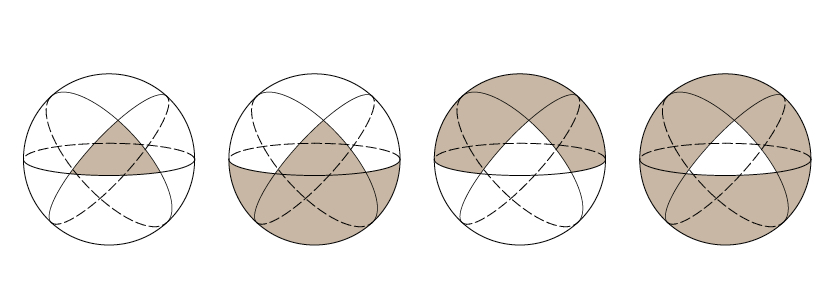
\includegraphics[width=0.9\textwidth]{kugel/Dreieckarten.jpg}
    \captionof{figure}{Dreiecksarten auf der Kugeloberfläche}
\end{center}

\subsection{Allgemeine Kugeldreiecke}

Ähnlich dem Dreieck in der Ebene hat das Dreieck auf der Kugel Seiten und Winkel. Allerdings werden die Seiten nicht in einer Länge angegeben sondern im Bogenmass. Auch hat das Dreieck auf der Kugel nicht zwingend $180^{\circ}$, die Winkelsumme liegt zwischen $180^{\circ}$ und zu $540^{\circ}$.

\subsection{Kugelzweieck}

Zwei Grosskreise auf der Kugeloberfläche zerlegen diese in vier gleich grosse Kugelzweiecke. 
Jedes dieser Dreieckseiten hat die Länge
$180^{\circ}$ oder $\pi$.
Der Flächeninhalt wird dabei nur durch den Winkel $\alpha$ zwischen den beiden Grosskreisen bestimmt.

\begin{center}
        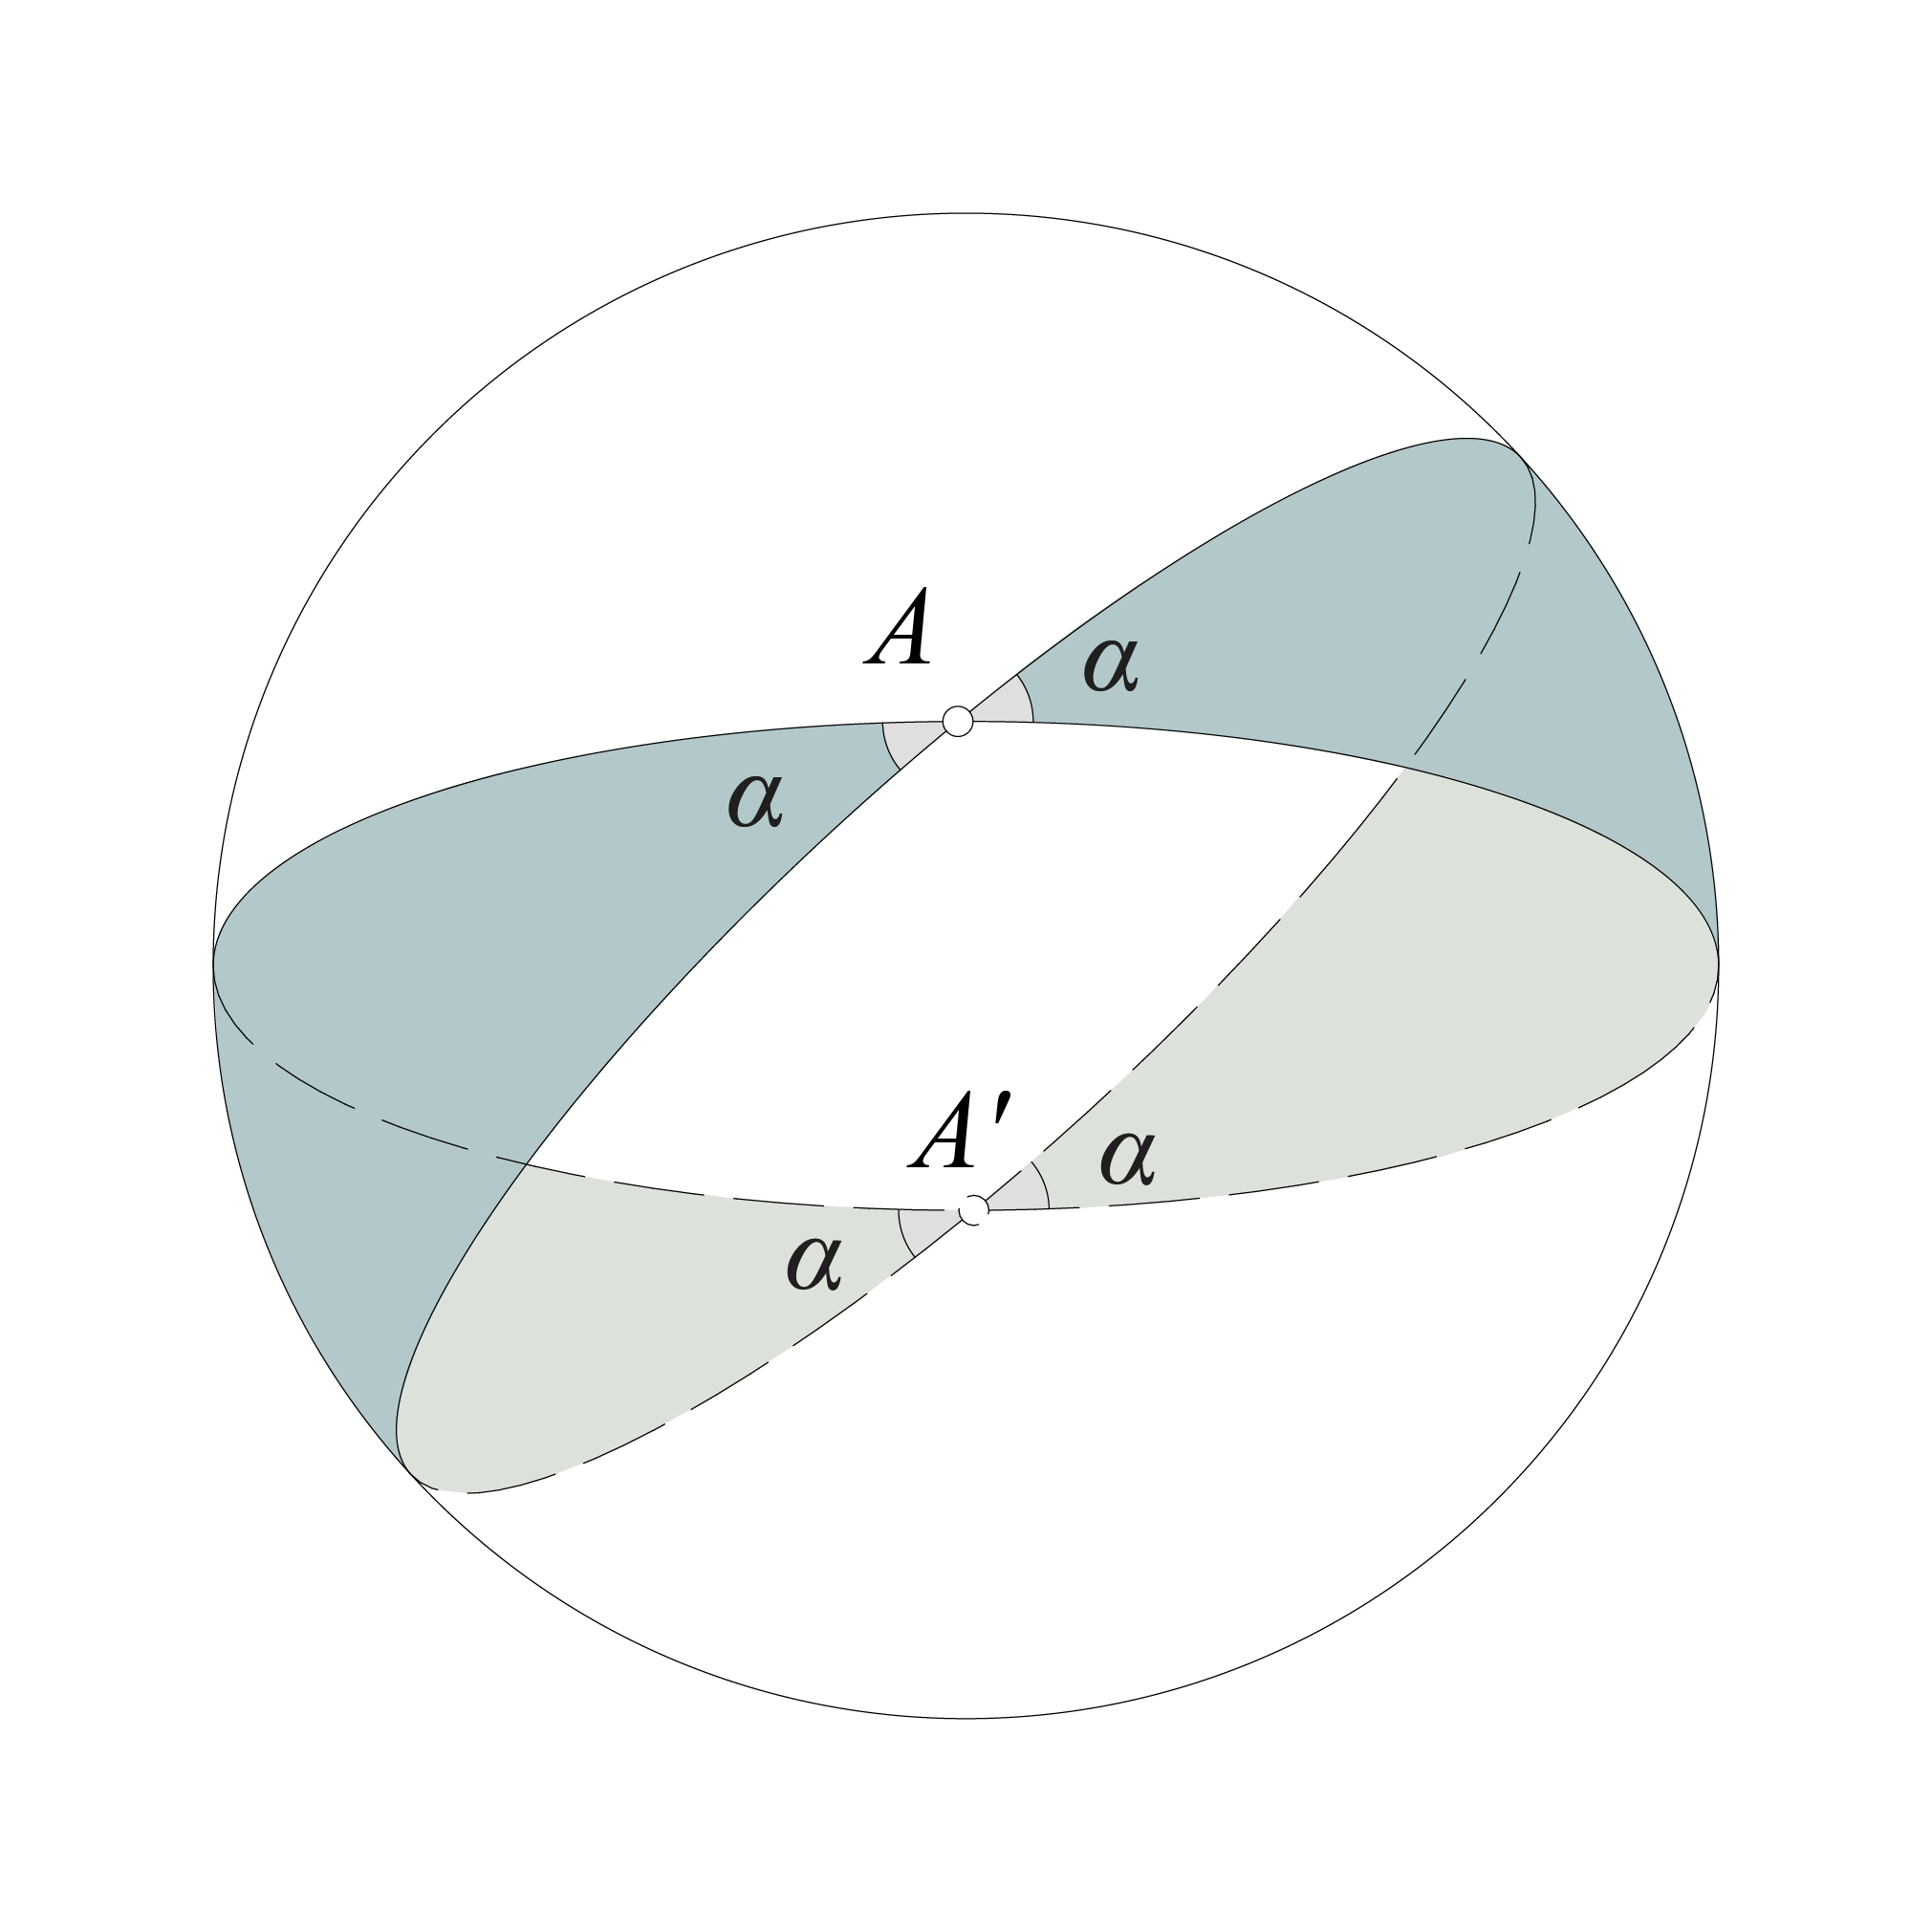
\includegraphics[width=0.3\textwidth]{kugel/Zweieck.jpg}
    \captionof{figure}{Bildung von Zweiecken durch Grosskreise}
\end{center}

Um den Flächeninhalt des Zweiecks zu erhalten, benötigen wir zuerst den Flächeninhalt der gesamten Kugel
\begin{align*}
A_{ Kugel } &= 4 \pi r^{2}
\end{align*}

Den Flächeninhalt der Kugel $A_{ Kugel }$ müssen wir noch mit dem Kugelsegment des Winkels $\alpha$ multiplizieren um dem Flächeninhalt des Zweiecks zu erhalten

\begin{equation}
A_{ Zweieck } = 4 \pi r^{2} \cdot \frac{ \alpha }{ 2 \pi }
\end{equation}

HIER NOCH EIN SATZ

\subsection{Eulersche’ Dreiecke}

Legt man drei Grosskreise auf eine Kugeloberfläche, bilden sich dabei acht Dreiecke. 
Ein solches Dreieck heisst Eulersches’Dreieck\footnote{%
Leonard Euler (1707-1783), berühmter Schweizer Mathematiker und Physiker. 
Nicht Eulersche’Dreiecke erhält man, indem man das Äussere des Dreieckes ABC betrachtet.}.
Diese Dreiecke werden weder durch die Verlängerung ihrer Seiten durchschnitten, 
noch haben sie Dreiecksseiten welche grösser als $180^{\circ}$ sind.

\begin{center}
        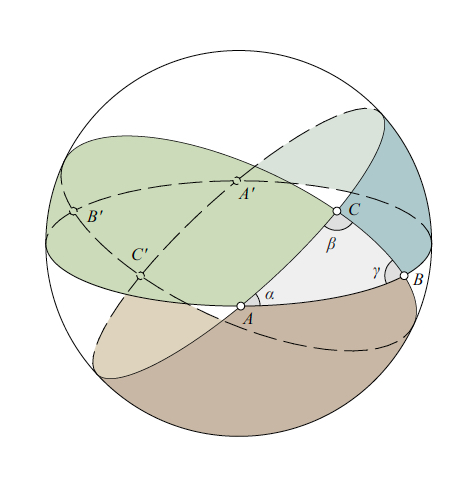
\includegraphics[width=0.4\textwidth]{kugel/Zweiecke.jpg}
    \captionof{figure}{Drei Grosskreise bilden ein sphärisches Dreieck}
\end{center}

In den nachstehenden Erklärungen und Herleitungen, sprechen wir ausschliesslich von Eulerschen’Dreiecken, da die umgeformten Winkelsätze der ebenen Trigonometrie nur auf diese Art von Kugeldreiecken angewendet werden kann.

$A_{ \overline{ ABC }}$ ist die Fläche des Dreieckes auf der Kugeloberfläche
In der ebenen Trigonometrie liegt die Winkelsumme eines Dreiecks bei
$180^{\circ}$.

Anders aber in der sphärischen Trigonometrie. Obschon sie einige Gemeinsamkeiten zur ebenen Trigonometrie aufweist, kann man nicht alles übernehmen.
So auch nicht wie Winkelsumme in einem sphärischen Dreieck.
Diese liegt bei:

\[
\begin{aligned}
\pi
&-
3\pi
&
&\text{\bigg \vert}
&
180^{\circ}
&-
540^{\circ}
\end{aligned}
\]

daraus lässt sich ableiten, das ein einzelner Winkel nicht grösser als $\pi$ oder $180^{\circ}$ sein darf. Ansonsten ist es kein Eulersches’Dreieck und wir dürfen die sphärische Trigonometrie nicht anwenden.\\
Wichtig anzumerken ist, dass die Seiten immer in Radiant beschrieben werden und nicht im Längenmass Meter wie wir es uns gewohnt sind. 
Bei den Dreiecksseiten handelt es sich um Kreisbögen und keine Strecken.

\section{Flächeninhalt sphärischer Dreiecke}

Der Flächeninhalt des Dreiecks $A_{ \triangle{ ABC }}$ berechnet sich aus den Winkeln $\alpha$, $\beta$, $\gamma$ und dem Kugelradius $r$ im Quadrat.
\begin{align*}
A_{ \triangle{ ABC }} &= (\alpha + \beta + \gamma) \cdot r^2
\end{align*}

\begin{center}
        \includegraphics[width=0.3\textwidth]{kugel/Beispielbild.jpg}
    \captionof{figure}{Bild FLäche dreieck}
\end{center}

Dies lässt sich folgendermassen herleiten: \\
Als erstes berechnen wir die Flächeninhalte der Zweiecke A, B und C

\begin{align*}
\text{Zweieck A}
&=
\triangle{ABC} + \triangle{A'BC} = 2 \alpha r^{ 2 } = A_{ \alpha }\\
\text{Zweieck B}
&=
\triangle{ABC} + \triangle{AB'C} = 2 \beta r^{ 2 } = A_{ \beta }\\
\text{Zweieck C}
&=
\triangle{ABC} + \triangle{ABC'} = 2 \gamma r^{ 2 } = A_{ \gamma }
\end{align*}

Addiert man nun die Flächeninhalte der einzelnen Zweiecke, ist diese Fläche gleich gross wie die der halben Kugel und zweimal des sphärischen Dreiecks $A_{ \triangle{ ABC }}$.

\begin{align*}
A_{ \alpha } + A_{ \beta } + A_{ \gamma } &= \frac{ 4\pi r^{ 2 } }{ 2 } + 2A_{ \triangle{ ABC }}
\end{align*}

Dies lässt sich umformen in

\begin{align*}
2\alpha r^{ 2 } + 2\beta r^{ 2 } + 2\gamma r^{ 2 } &= \frac{ 4\pi r^{ 2 } }{ 2 } + 2A_{ \triangle{ ABC }} \parallel:2
\end{align*}

Durch vereinfachen der Gleichung erhalten wir

\begin{align*}
\alpha r^{ 2 } + \beta r^{ 2 } + \gamma r^{ 2 } &= \pi r^{ 2 } + A_{ \triangle{ ABC }} \parallel-\pi r^{ 2 }\\
\end{align*}

Wir haben damit den folgenden Satz bewiesen:

\begin{satz}[\textit{Hallo ich heisse Flächeninhalt}]
\label{skript:kugel:satz:Flaecheninhalt}
\index{Flaecheninhalt}
\end{satz}

\begin{align*}
A_{ \triangle{ ABC }} &= r^{ 2 }\left(\alpha + \beta + \gamma - \pi\right) 
\end{align*}


\section{Sphärischer Exzess}
Anders als bei Dreiecken in der Ebene, ist die Winkelsumme bei sphärischen Dreiecken immer \textgreater \,  $\pi$.

\begin{align*}
\pi < \alpha + \beta + \gamma
\end{align*}

Der sphärische Exzess gibt dabei an, wie stark die Winkelsumme von $\pi$ abweicht.

\begin{align*}
\pi + \epsilon &= \alpha + \beta + \gamma \\
\end{align*}

Lösen wir nach $\epsilon$ auf:

\begin{equation}
\epsilon = \alpha + \beta + \gamma - \pi
\end{equation}

Zur Berechnung des Flächeninhalts eines sphärischen Dreiecks berechnet man demzufolge den sphärischen Exzess multipliziert mit dem Radius im Quadrat.
Dies zeigt, dass der Exzess direkt mit dem Flächeninhalt $A$ eines sphärischen Dreiecks zusammenhängt

\begin{align*}
\epsilon = \frac{A_{ \overline{ ABC }}}{r^2}
\end{align*}

\begin{center}
        \includegraphics[width=0.3\textwidth]{kugel/Beispielbild.jpg}
    \captionof{figure}{Bild Sphärischer Exzess}
\end{center}

Bei allgemeinen Kugeldreiecken gilt demnach:

\begin{align*}
\pi < \alpha + \beta + \gamma < 5\pi (900^{\circ})
\end{align*}


Bei Eulerschen’ Kugeldreiecken

\begin{align*}
\pi < \alpha + \beta + \gamma < 3\pi (540^{\circ})
\end{align*}

Der sphärische Exzess wird gleichmässig auf alle Winkel des Dreiecks aufgeteilt.

Bezieht man den sphärischen Exzess und die Formel des Flächeninhaltes auf die Erde und somit eine Kugel, kann man mit Hilfe eines beliebigen sphärischen Dreieckes und dessen Flächeninhalt auf den Radius der Kugel schliessen.

\subsection{Grenzfall - Satz von Legendre}

Würde der sphärische Exzess in der ebenen Trigonometrie angewendet, wäre dieser = 0.
Bei sehr kleinen sphärischen Dreiecken lässt sich dies annähernd wie in der ebenen Trigonometrie betrachten

\begin{quote} \textit{Ein kleines sphärisches Dreieck kann näherungsweise 
wie ein ebenes Dreieck mit denselben Seiten berechnet 
werden, wenn alle Winkel des ebenen Dreiecks die um 
je ein Drittel des sphärischen Exzesses verminderten 
Winkel des sphärischen Dreiecks nimmt.} \end{quote}
\begin{flushright} - Adrien-Marie Legendre (1752-1833), Paris 1787
\end{flushright}

Diese Aussage zeigt den Zusammenhang zwischen der 
Trigonometrie in der Ebene sowie in auf der Kugel
auf. Im speziellen bei sehr kleinen sphärischen 
Dreiecken ist die Winkelsumme nur unwesentlich 
grösser als $180^{\circ}$. 
Wichtig anzumerken ist, dass der Satz von Legendre 
für grosse, aber endliche Radien $r$ gilt.

\begin{center}
        \includegraphics[width=0.3\textwidth]{kugel/Beispielbild.jpg}
    \captionof{figure}{Bild Krümmung Gross und Klein}
\end{center}


\section{Sphärisch Analoge Winkelfunktionen}
Euklid von Alexandria\footnote{%
Euklid war ein griechischer Mathematiker. Er lebte wahrscheinlich 3 Jahrhunderte vor Christus. In seinem berühmtesten Werk \textit{Euklids Elemente} fasst er die Arithmetik und Geometrie seiner Zeit zusammen. \textit{Euklids Elemente} war 2000 Jahre lang als Lehrbuch in gebrauch und war bis Mitte des 19. Jahrhunderts nach der Bibel das weit verbreitetste Buch der Weltliteratur.}  beschrieb die Grundbegriffe der ebenen Geometrie mittels Punkt, Geraden, Ebene, Winkel und Dreieck. Ebendiese Dreiecke lassen sich mithilfe der ebenen Trigonometrie beschreiben. Dabei gelten die uns bekannten trigonometrischen Winkelfunktionen:\\

\text{Sinussatz:}
\begin{align*}
\frac{ a }{ sin(\alpha) } &= \frac{ b }{sin(\beta)} = \frac{ c }{ sin(\gamma) } = \frac{abc}{2A} = 2r\\
\end{align*}

\text{Cosinussatz:}
\begin{align*}
c^{ 2 } &= a^{ 2 } + b^{ 2 } - 2ab\cdot cos(\gamma)\\
b^{ 2 } &= a^{ 2 } + c^{ 2 } - 2ab\cdot cos(\beta)\\
a^{ 2 } &= b^{ 2 } + c^{ 2 } - 2ab\cdot cos(\alpha)
\end{align*}

Um diese Winkelfunktionen auf der Kugeloberfläche anwenden zu können, benötigen wir die sphärische Trigonometrie. Die oben beschriebenen Sätze lassen sich auf der Kugel nicht anwenden, sie werden aber als Grundlage und Gedankenstütze zur Herleitung der Sätze für das Kugeldreieck benötigt.

\subsection{Sphärischer Sinussatz}

\begin{center}
        \includegraphics[width=0.3\textwidth]{kugel/Beispielbild.jpg}
    \captionof{figure}{Bild Sinussatz}
\end{center}


Wir betrachten das folgende sphärische Dreieck auf einem Teilstück der Kugeloberfläche mit dem Radius $R= \overline{MA} = \overline{MB} = \overline{MC}$. Danach fügen wir ein ebenes Dreieck $\triangle=\overline{ADE}$ in das Kugelstück ein, welches den Eckpunkt $A$ des sphärischen Dreiecks beinhaltet und eine Abbildung des sphärischen Dreieckes bildet.

Es gilt

\begin{align*}
\overline{AD} &= R \cdot sin (c) \\
hA = \overline{AF} &= \overline{AD} \cdot sin(\beta) = R \cdot sin(c) \cdot sin(\beta)  
\end{align*}

Aus einer anderen Sichtweise kann man auch schreiben

\begin{align*}
h_{A} = R \cdot sin(b) \cdot sin(\gamma)  
\end{align*}

Durch gleichsetzen dieser Ausdrücke ergibt sich

\begin{align*}
R \cdot sin(c) \cdot sin(\beta) &= R \cdot sin(b) \cdot sin(\gamma) \\
\Rightarrow \quad \quad
sin(c) \cdot sin(\beta) &= sin(b) \cdot sin(\gamma) \\
\Rightarrow \quad \quad
\frac{sin (b)}{sin (c)} &= \frac{sin (\beta)}{sin (\gamma)}
\end{align*}

Analog dazu könnte man auch die Höhe $h_{B}$ nehmen und würde erhalten

\begin{align*}
sin(c) \cdot sin(\alpha) &= sin(a) \cdot sin(\gamma) \\
\Rightarrow \quad \quad
\frac{sin (a)}{sin (c)} &= \frac{sin (\alpha)}{sin (\gamma)}
\end{align*}

Aus diesen Erkenntnissen lässt sich der Sinussatz zusammenfassen

\begin{satz}[\textit{Der sphärische Sinussatz verhaltet sich wie der Sinus der Seiten wie der Sinus der Gegenwinkel, dies lässt sich beschreiben}]
\label{skript:kugel:satz:Sinussatz}
\index{Sinussatz}
\end{satz}

\begin{align*}
\sin(a) : \sin(b) : \sin(c) &= \sin(\alpha) : \sin(\beta) : \sin(\gamma) \\
 \\
\frac{sin(\alpha)}{sin(a)} &= \frac{sin(\beta)}{sin(b)} = \frac{sin(\gamma)}{sin(c)}
\end{align*} 


\subsection{Seitenkosinussatz}

Es sei das Stück einer Kugel mit dem sphärischen Dreieck $ABC$ und den Winkeln $\alpha, \beta, \gamma$ und den Seiten $a, b, c$. Die Senkrechten durch den Mittelpunkt, schneiden dabei die Eckpunkte des sphärischen Dreieckes. Wir erstellen in der Ebene ein Ähnliches Dreieck $A’B’C’$.

\begin{center}
        \includegraphics[width=0.3\textwidth]{kugel/Beispielbild.jpg}
    \captionof{figure}{Bild Seitenkosinus}
\end{center}

Dabei lassen sich die Strecken nach den uns bekannten Regeln der Trigonometrie beschreiben:

\begin{align*}
\overline{C'A'} &= d\cdot {tan(b)} \\
\overline{C'B'} &= d\cdot {tan(a)} \\
\overline{MA'} &= \frac{ d }{cos(b)} \\
\overline{MB'} &= \frac{ d }{cos(a)}
\end{align*} 

Dabei schreibt sich der Kosinussatz der Ebene wie folgt

\begin{align*}
c^{ 2 } &= a^{ 2 } + b^{ 2 } - 2ab \cdot cos(\gamma)
\end{align*}

Daher gilt für das Dreieck $A’B’C’$

\begin{align*}
\triangle \overline{A'B'}^{ 2 } &= \overline{ C'B' }^{ 2 } + \overline{ C'A' }^{ 2 } - 2 \cdot \overline{C'B'} \cdot \overline{ C'A' } \cdot cos(\gamma) \\
\Rightarrow \quad \quad
\triangle \overline{A'B'}^{ 2 } &= d^{ 2 } \cdot \left(\left(tan^{ 2 }(a) + tan^{ 2 }(b)\right) - 2\cdot tan(a) \cdot tan(b) \cdot cos(\gamma)\right)
\end{align*}


das gilt ebenso für das Dreieck $MA’B’$

\begin{align*}
\triangle \overline{ MA'B' }^{ 2 } &= \overline{ MB' }^{ 2 } + \overline{ MA' }^{ 2 } - 2\cdot \overline{ MB'} \cdot \overline{ MA' } \cdot cos(c) \\
\Rightarrow \quad \quad
\overline{ MA'B'}^{ 2 } &= \left(\frac{ d }{ cos(a) }  \right)^{ 2 } + \left(\frac{ d }{ cos(b)}  \right)^{ 2 } - 2 \cdot \frac{ d }{ cos(a)} \cdot \frac{ d }{ cos(b)} \cdot cos(c)
\end{align*}


Im Einheitskreis betrachtet ergibt dies

\begin{align*}
\overline{ MA'B' }^{ 2 } &= d^{ 2 } \cdot \left(\left(\frac{ 1 }{ cos(a) }  \right)^{ 2 } + \left(\frac{ 1 }{ cos(b) }  \right)^{ 2 } - 2 \cdot \frac{ 1 }{ cos(a)} \cdot \frac{ 1 }{ cos(b)} \cdot cos(c)\right)
\end{align*}


Durch berücksichtigen von $\frac{1}{\cos^{2}(x)}=\tan^{2}(x)+1$ folgt

\begin{align*}
\overline{ A'B'}^{ 2 } &= d^{ 2 } \cdot \left(\left(tan^{ 2 }(a) + tan^{ 2 }(b)\right) - 2 \cdot \frac{ 1 }{ cos(a)} \cdot \frac{ 1 }{ cos(b)} \cdot cos(c)\right) \\
\Rightarrow \quad \quad
\overline{ A'B'}^{ 2 } &= d^{ 2 } \cdot \left(\left(tan^{ 2 }(a) + 1\right) + \left(tan^{ 2 }(b) + 1\right) - \left(2 \cdot \frac{cos(c)}{cos(a) \cdot cos(b)}\right)\right)
\end{align*}


Durch gleichsetzen dieser beiden Ausdrücke folgt

\begin{align*}
2 \cdot tan(a) \cdot tan(b) \cdot cos(\gamma) &= -2+2 \cdot \frac{cos(c)}{cos(a) \cdot cos(b)}
\end{align*}

Durch umformen durch $\tan(a)=\frac{\sin(a)}{\cos(a)}$ und der Multiplikation mit  $\frac{1}{2}$ ergibt sich

\begin{align*}
\frac{\sin(a)}{\cos(a)} \cdot \frac{\sin(b)}{\cos(b)} \cdot \cos(\gamma) &= -1 + \frac{\cos(c)}{\cos(a) \cdot \cos(b)}
\end{align*}

Durch vereinfachen der Formel erhalten wir den Seitenkosinussatz der Seite $c$

\begin{align*}
\cos(a) \cdot \cos(b) + \sin(a) \cdot sin(b) \cdot \cos(\gamma) = \cos(c)
\end{align*}

Durch zyklische Vertauschung der Variablen erhält man den 

\begin{satz}[\textit{Im sphärischen Dreieck ist der Kosinus einer Seite gleich der Summe der Kosinusprodukte der beiden anderen Seiten und dem mit dem Kosinus des eingeschlossenen Winkels multiplizierten Sinusprodukt dieser Seiten}]
\label{skript:kugel:satz:Seitenkosinussatz}
\index{Seitenkosinussatz}
\end{satz}


\begin{align*}
{\cos a} &= {cos(b)} \cdot {cos(c)} + {sin(b)} \cdot {sin(c)} \cdot {cos(\alpha)}\\
{cos(b)} &= {cos(c)} \cdot {cos(a)} + {sin (c)} \cdot {sin(a)} \cdot {cos(\beta)}\\
{cos(c)} &= {cos(a)} \cdot {cos(b)} + {sin(a)} \cdot {sin(b)} \cdot {cos(\gamma)}\\
\end{align*}


ABSCHLUSSATZ

\subsection{Winkelkosinussatz}

Wenden wir den sphärischen Seitenkosinussatz auf dem Polardreieck an, erhalten wir
\begin{align*}
{\cos (a)} = {\cos (b)} \cdot {\cos (c)} + {\sin(b)} \cdot {\sin(c)} \cdot {\cos (\alpha)}
\end{align*}

\begin{center}
        \includegraphics[width=0.3\textwidth]{kugel/Beispielbild.jpg}
    \captionof{figure}{Bild Winkelkosinus/Polardreieck}
\end{center}

Durch die Beziehung zwischen dem Polardreieck und einem sphärischen Dreieck, können wir den Seitenkosinussatz folgendermassen umformen
\begin{align*}
{\cos (\pi-\alpha)} &= {\cos (\pi-\beta)} \cdot {\cos (\pi-\gamma)} + {\sin(\pi-\beta)} \cdot {\sin(\pi-\gamma)} \cdot {\cos (\pi-a)}
\end{align*}

Durch die Quadrantenbeziehung der trigonometrischen Funktionen im Einheitskreis folgt

\begin{align*}
\sin (\pi-\alpha) &= sin(\alpha)\\
\cos (\pi-\alpha) &= - cos (\alpha)\\
\end{align*}

Daher ergibt sich

\begin{align*}
{-\cos (\alpha)} &= {-\cos (\beta)} \cdot {-\cos (\gamma)} + {\sin(\beta)} \cdot {\sin(\gamma)} \cdot {-\cos (a)}
\end{align*}

Durch vertauschen der Vorzeichen erhalten wir den Winkelkosinussatz

\begin{satz}[\textit{Im sphärischen Dreieck ist der Kosinus eines Winkels gleich der Summe aus dem negativen Produkt der Kosinus der beiden anderen Winkel und dem mit dem Kosinus der gegenüberliegenden Seite multiplizierten Sinusprodukt der beiden anderen Winkel.}]
\label{skript:kugel:satz:Winkelkosinussatz}
\index{Winkelkosinussatz}
\end{satz}

\begin{align*}
{\cos (\alpha)} &= {-\cos(\beta)} \cdot {\cos(\gamma)} + {\sin (\beta)} \cdot {\sin(\gamma)} \cdot {\cos(a)}\\
{\cos (\beta)} &= {-\cos(\gamma)} \cdot {\cos(\alpha)} + {\sin (\gamma)} \cdot {\sin(\alpha)} \cdot {\cos(b)}\\
{\cos (\gamma)} &= {-\cos(\alpha)} \cdot {\cos(\beta)} + {\sin (\alpha)} \cdot {\sin(\beta)} \cdot {\cos(c)}\\
\end{align*}

ABSCHLUSSATZ

\section{Dualität auf der Kugel}

Durch die Herleitung des Winkelkosinussatzes haben wir zugleich die Dualität auf der Kugel bewiesen.

\begin{satz}[\textit{Die sphärische Geometrie ist eine projektive Geometrie. In der projektiven Geometrie lassen sich alle Sätze dualisieren, das heisst, die Begriffe Punkt und Geraden werden vertauscht; demzufolge auch Längen und Winkeln}]
\label{skript:kugel:satz:Dualitaet}
\index{Dualitaet}
\end{satz}

\begin{center}
        \includegraphics[width=0.3\textwidth]{kugel/Beispielbild.jpg}
    \captionof{figure}{Bild Dualität}
\end{center}

Dualisiert man nun als Beispiel einen Punkt und eine Gerade, bleibt die Beziehung zwischen dem Punkt und der Geraden erhalten.
Nimmt man nun den Punkt $A$ welcher auf der Geraden $b$ liegt, so verläuft die Duale Gerade $a$ durch den zur Geraden $b$ dualen Punkt $B$. 
Aber nicht nur die Beziehungen zwischen Punkten und Längen bleiben erhalten. Auch die Winkel und Längen gehen ineinander über wie wir es im Beweis des Winkelkosinussatzes gesehen haben.
Der Winkel $\gamma$ zwischen den beiden Seiten a und b entspricht auf der Einheitskugel dem Abstand zwischen den zu der Geraden dualen Punkten A und B.

\section{Navigation auf See}
Das besondere an Seekarten ist die Inhaltliche Ausrichtung. Anders wie Landkarten muss sie Informationen enthalten welche für den Kapitän und seine Besatzung von grosser Bedeutung sind. Vor allem in Küstennähe ist das navigieren eines Schiffes besonders gefährlich. So enthalten Seekarten etwas über Wassertiefen, Bodenbeschaffenheiten, Gezeiten, Küstenlinien, Landzungen und Windrichtungen.
Der Hauptunterschied dabei ist, das auf der Landkarte feste Positionen definiert und aufgezeigt werden, das einzige was sich verändert ist der Reisende selbst. Bei der Seekarte ist das anders, es werden veränderliche Einwirkungen der Natur festgehalten.

Dieser kleine Unterschied zeigt die Notwendigkeit auf, die Position und den Kurs seines Schiffes auf See immer ermitteln zu können.


\section{Geographische Koordinaten}

Nachdem klar war, das die Erde eine Kugel ist, wurde diese in ein Gradnetz aufgeteilt. Dabei wurden die Angaben für eine exakte Ortsbestimmung klar definiert und die bis heute gültigen Koordinaten bestimmt.
Dabei muss man sich nochmals in Erinnerung rufen, dass sich die Erde in 24h einmal um ihre eigene Achse dreht. Nach $360 ^{\circ}$ 
und somit einer vollen Umdrehung, steht sie wieder in ihrer Ursprungsposition und ein neuer Tag beginnt.

Die Koordinaten setzen sich aus folgenden Komponenten zusammen:

\[
\begin{aligned}
&\text{Grad } (^{\circ})
&
&\text{\bigg \vert}
&
&\text{Bogenminuten } (`)
&
&\text{\bigg \vert}
&
&\text{Bogensekunden } (``)
\end{aligned}
\]

Die Erdoberfläche wurde in je 360 Breiten- und Längengrade eingeteilt. Die Breitengrade haben zueinander einen Abstand von 111.31 km, dies entspricht auch dem Abstand der Längengrade am Äquator mit Zunehmender Nähe zu den Polen, nimmt dieser Abstand ab.

\[
\begin{aligned}
&1^{\circ}
&
&\text{\bigg \vert}
&
&4 \text{ Minuten}
&
&\text{\bigg \vert}
&
&111.31\text{ km}
\end{aligned}
\]

Berechnet man nun die Erdumdrehung von 360°, erhält man genau den Erdumfang am Äquator: \begin{align*} 40’074 \text{ km.}\end{align*}

Dabei geben die Bogenminuten und -sekunden dem Standort die gewünschte Exaktheit. Mit den vollständigen Koordinaten lässt sich der Standort auf einer Landkarte exakt bestimmen und einzeichnen.

\subsection{Erdachsenneigung}

Die Erdachse oder auch Rotationsachse der Erde ist um ca. $23.5^{\circ}$ geneigt.
Dadurch lassen sich Phänomene wie die vier Jahreszeiten sowie die unterschiedliche Längen der einzelnen Tage herleiten.
Für die nautische Navigation hat dies eine grosse Bedeutung, da je nach Neigung andere Sterne zu sehen sind, auch die Sonne ist an einem anderen Ort am Himmel zu finden.

\begin{center}
        \includegraphics[width=0.3\textwidth]{kugel/Beispielbild.jpg}
    \captionof{figure}{Bild Erdneigung}
\end{center}

Der Himmelsäquator ist die Linie, die orthogonal zur Sonne verläuft.
Die Ekliptil-Linie ist die Linie, die orthogonal zur Erdachse verläuft.
Der Schnittpunkt dieser Kreise wird als Frühlings- / Herbstpunkt bezeichnet und ist jeweils am 21. März / 21. Oktober des Jahres.
Der Frühlingspunkt $\Upsilon$ wird oft als Gestirnspunkt im nautischen Dreieck verwendet, genaueres wird im Kapitel zum nautischen Dreieck erklärt.


\subsection{Zeitzonen der Erde}
Wenn man nun die verschiedenen Zeitzonen der Erde betrachtet, macht die Verschiebung von jeweils einer Stunde durchaus Sinn, es lässt sich auf die Längengrade schliessen.
Zwischen den verschiedenen Zeitzonen liegen 15 Längengrade:
\begin{align*}
\text{15 Längengrade à 4 Minuten = 60 Minuten Zeitverschiebung = ca. 1665 km}
\end{align*}

Dabei ist die Zeitzone in welcher Mitte sich der Greenwich Meredian befindet die \textit{Greenwich Mean Time (GMT)} welche bis 1928 als Weltzeit galt. Im Jahr 1972 wurde diese umbenannt in die \textit{Coordinated Universal Time (UTC)} und wir von da an als Weltzeit $\pm$ 0.00 verwendet.


\section{Der Breitengrad}
Die Breitengrade bilden die bereits genannten Kleinkreise auf der Kugeloberfläche. Sie verlaufen in einem Abstand von genau 111 km parallel zum Äquator. Dabei stellt  dieser genau die Mitte zwischen Nord- und Südpol dar und teilt die Erdkugel in zwei gleiche Hälften. Somit wird von nördlicher und südlicher Breite gesprochen, je nach dem auf welcher Halbkugel man sich befindet.

\begin{center}
        \includegraphics[width=0.3\textwidth]{kugel/Beispielbild.jpg}
    \captionof{figure}{BILD SKIZZE DER GEOGRAFISCHEN BREITE ERDKUGEL}
\end{center}


\subsection{Geografische Breite $\phi$}
\begin{definition}
Die geografische Breite eines Standortes ist nichts anderes, als der Winkel am Erdmittelpunkt zwischen der Ebene des Äquators und der Geraden zum Standpunkt auf der Erdoberfläche.
\end{definition}

\begin{center}
        \includegraphics[width=0.3\textwidth]{kugel/Beispielbild.jpg}
    \captionof{figure}{Bild}
\end{center}


\subsection{Navigation mit den Breitengraden}
Da der Breitengrad bereits sehr früh ziemlich präzise bestimmt werden könnte, nutzten bereits die Seefahrer um Christoph Kolumbus den Breitengrad zur Navigation ihrer Flotten.
Den dieser lässt sich ziemlich einfach aus dem höchsten Sonnenstand oder einem Fixstern bestimmen. Dabei wird mit einem Jakobsstab\footnote{%
Der Jakobsstab ist ein früheres astronomisches Instrument zur Winkelmessung und wurde vor allem in der Seefahrt verwendet. Er ist in der Nautik der Vorläufer des Sextanten.} (später Sextant\footnote{%
Der Sextant ist ein nautisches Messinstrument zur Winkelmessung von Horizont und Fixstern (Gestirn)}) der Winkel zwischen dem Horizont und dem Fixstern gemessen. Der Winkel welchen man erhält, zieht man von 90° ab und erhält somit die geografische Breite. \\

\begin{center}
        \includegraphics[width=0.3\textwidth]{kugel/Beispielbild.jpg}
    \captionof{figure}{Bild}
\end{center}

Wenn man sich auf der Nordhalbkugel befindet, ist der Polarstern ein sehr guter Fixstern. Befindet sich ein Schiff nun sehr nahe am Nordpol, steht dieser nahezu senkrecht am Himmelszelt bei $90^{\circ}$. Würde es aber nahe dem Äquator stehen, erscheint dieser am Horizont bei $0^{\circ}$.

\subsection{Korrekturbeiwert}
Die Breitengrade auf der Erde haben nicht alle den selben Radius. Daher segelt man am Äquator viel länger dem Breitengrad entlang um zum nächsten Längengrad zu kommen wie in der nähe des Nord- oder Südpols.

\[
\begin{aligned}
&\text{1} (^{\circ})
&
&\text{\bigg \vert}
&
&\text{4 Minuten}
&
&\text{\bigg \vert}
&
&\text{111.13 km}
\end{aligned}
\]

\[
\begin{aligned}
&\text{0.25} (^{\circ})
&
&\text{\bigg \vert}
&
&\text{1 Minute}
&
&\text{\bigg \vert}
&
&\text{27.78 km}
\end{aligned}
\]

\[
\begin{aligned}
&\text{0.004166} (^{\circ})
&
&\text{\bigg \vert}
&
&\text{1 Sekunde}
&
&\text{\bigg \vert}
&
&\text{463m}
\end{aligned}
\]

Um die Minderung der Strecke zu erhalten, müssen wir den Cosinus des gemessenen Breitengrades berechnen und diesen mit der Abweichung auf dem Äquator von 1 Sekunde multiplizieren.

\begin{center}
        \includegraphics[width=0.3\textwidth]{kugel/Beispielbild.jpg}
    \captionof{figure}{Bild}
\end{center}

\[
\begin{aligned}
&\cos 90^\circ \cdot 463m = 463m
&
&\text{\bigg \vert}
&
&\cos 50^\circ \cdot 463m = 297.61m
&
&\text{\bigg \vert}
&
&\cos 0^\circ \cdot 463m = 0m
\end{aligned}
\]

Dies zeigt auf je näher man den Polen ist, desto weniger weit muss man Segeln um den nächsten Längengrad zu erreichen.

\section{Der Längengrad}
Die Längengrade bilden die bereits genannten Grosskreise auf der Kugeloberfläche.
Sie schneiden den Äquator im rechten Winkel, haben dort einen Abstand von 111 km zueinander und verbinden die Pole. Anders wie bei der geografischen Breite, ist in der Natur kein Längengrad gegeben welcher den Nullpunkt darstellt.

\begin{center}
        \includegraphics[width=0.3\textwidth]{kugel/Beispielbild.jpg}
    \captionof{figure}{Bild}
\end{center}


\subsection{Geografische Länge $\lambda$}
\begin{definition}
Die geografische Länge ist der Winkel an der Erdachse zum Nullmeridian.
\end{definition}

\subsection{Navigation mit den Längengraden}
Die geografische Länge lässt sich nicht so einfach bestimmen wie deren Breite. Für die Berechnung auf See benötigt man eine Referenzzeit eines Ortes mit bekannter Länge.
In der Zeit der Entdecker gab es noch keine mechanischen Uhren. Die Sonnenuhr war zudem ungeeignet, da diese nur die Uhrzeit am Standort mass und nicht die am Referenzort selbst. Die erste Pendeluhr wurde erst Mitte des 17. Jahrhunderts erfunden, was in der Schifffahrt aber auch nicht die Lösung brachte.\\
Pendeluhren auf einem Schiff sind ungeeignet, da das Pendel mit dem Wellengang aus dem Takt gebracht wird und somit die Uhr falsch geht.
Zu ungenau und gegen äussere Erschütterungen zu empfindlich waren später auch die federgetriebenen Uhren und die Unruh. Dazukamen die verschiedenen Klimazonen welche ein Schiff zu durchqueren hatten. Das Metall zog sich viel zu fest zusammen oder dehnte sich aus, was dazu führte das die Uhr unregelmässig lief.

Das sogenannte „Längenproblem“ stellte nicht nur bei der Navigation auf See ein Problem dar, es ergaben sich auch wirtschaftliche Konsequenzen. Die Schiffe mussten bis zur gewünschten geografischen Breite navigieren und segelten dann den Breitengrad entlang. Dabei waren die Schiffe oft Wochenlang unterwegs und segelten die „Breiten ab“ um an die gewünschte Position zu kommen. Dies führte zu erheblichen Zeitverlusten und viel längeren Reisezeiten.


\section{The Board of Longitude - Das Längenproblem}
Das Längenproblem beschäftigte alle grossen Seefahrernationen Europas. Die fehlenden Längengrade bei der Navigation führten zu vielen Schiffsunglücken. Dies zeigt auch die Dringlichkeit der Lösung dieses Problems auf: Nicht selten kam es vor, das sich auf den verloren gegangenen Schiffen Schätze in der Höhe von halben britischen Staatshaushalten befanden. Der Verlust solcher Schiffe war enorm.\\
Bereits um 1600 hatte der König von Spanien ein Preisgeld ausgeschrieben für denjenigen welcher eine Lösung für das Problem präsentieren konnte. Leider ohne Erfolg. \\

Nach einem tragischen Unglück im Jahr 1707 beidem der siegreiche Admiral Sir Cloudesley und seine 1’450 Mann sein Leben liessen, indem sie auf die Scilly-Inseln kurz vor Land’s End aufliefen und dabei die 21 Schiffe sanken, rückte das Problem wieder in den Vordergrund.
114 Jahre später, nach einer Petition von William Whiston und Humphry Ditton welche von Sir Isaac Newton und Edmond Halley untermauert wurde, reagierte das britische Parlament.
Es schrieb folgende Preisgelder für eine praktisch, brauchbare Lösung aus:\\

\begin{compactitem}
\item £ 20’000 - Abweichung von max. $\frac{1}{2}^{\circ}$
\item £ 15’000 - Abweichung von $\frac{2}{3}^{\circ}$
\item £ 10’000 - Abweichung von max. $1 ^{\circ}$
\end{compactitem}
\\
Im Kapitel der Korrekturbeiwertberechnung des Breitengrades haben wir erfahren, das eine Abweichung von $1 ^{\circ}$ am Äquator ca. 111km entsprechen - dies sind 60 Seemeilen.
Auf der Höhe des Ärmelkanals und damit London, beträgt die Abweichung nur noch 74km und somit 40 Seemeilen.//
Das Preisgeld entsprach einer enorm hohen Summe für diese Zeit. Der Kaufpreis für ein mittleres Schiff welches zur See fahren konnte lag bei etwa 1’500-2’500£, ein einzelner Arbeiter lebte mit 10£ im Jahr.
Würde man dieses Problem heute mit einer Abweichung von einem halben Grad lösen, erhielte man 2’840’000£ was etwa einem Wert von 3’600’000 Schweizer Franken entspräche. \\

Damit die Lösungsvorschläge kontrolliert und verwaltet werden konnten, wurde die Board of Longitude (Längenkommission) gegründet. Ihr gehörten die bedeutendsten Astronomen und Mathematiker dieser Zeit an, aber auch d



\subsection{John Harrison}

\begin{center}
        \includegraphics[width=0.3\textwidth]{kugel/JohnHarrison.jpg}
    \captionof{figure}{Bild John Harrison}
\end{center}





\begin{center}
        \includegraphics[width=0.2\textwidth]{kugel/HarrisonH4.jpg}
    \captionof{figure}{Bild Harrison's H4}
\end{center}


\subsection{Tobias Mayer}

\begin{center}
        \includegraphics[width=0.3\textwidth]{kugel/TobiasMayer.jpg}
    \captionof{figure}{Bild}
\end{center}

Tobias Mayers\footnote{%
Tobias Mayer (1723-1762) studierte nie an einer Universität und war trotzdem ein annerkannter Wissenschaftler seiner Zeit in den Bereichen Astronomie, Geo- und Kartograf, Mathematiker und Physiker.} 
 Mondkarten galten ein halbes Jahrhundertlang als unübertroffen. Der Ruhm galt aber hauptsächlich seinen Mondkarten welche er im Jahr 1755 in einer erweiterten Version dem britischen Parlament vorlegte.\\
Mit ihnen konnte man die Geografische Länge bis auf 5 Bogensekunden genau bestimmen. Dies entsprach am Äquator $0.5 ^{\circ}$, was wiederum eine Genauigkeit von 55.565km entsprach.\\
Eine Lösung für das Längenproblem war gefunden. Die Publikation seiner Mondtafeln fand 1767 unter dem Titel \textit{Theoria lunae juxta systema Newtonianum} in London statt, 5 Jahre nach Mayers Tod. 
Seine Witwe schickte die publizierten Mondkarten über die Universität Göttingen nach Grossbritannien. Sie erhielt von der britischen Regierung eine Prämie in der Höhe von £ 3’000.-.

Im Jahr 1935 wurde ein Krater auf der westlichen Mondvorderseite nach dem deutschen Astronomen benannt, er trägt fortan den Namen T.Mayer.

\begin{center}
        \includegraphics[width=0.3\textwidth]{kugel/Mondkarte.jpg}
    \captionof{figure}{Mondkarte}
\end{center}


\section{Nautisches oder Astronomisches Dreieck}
Ein sphärisches Dreieck an der Himmelskugel welches folgende Eckpunkte hat
- Zenit
- Himmelsnordpol
- Gestirn
nennt man nautisches Dreieck.\\

Es ist ein Hilfsmittel wenn es darum geht, den Standort seines Beobachtungspunktes auf dem offenen Meer herauszufinden oder den Standort eines Sterns zum bestimmten Zeitpunkt zu ermitteln.

\subsection{Das Horizontsystem (lokale Beobachtung)}


\subsubsection{Gestirnshöhe $h$}
Ist die sphärische Entfernung des Gestirns vom Horizont, gezählt nordwärts $+0^{\circ}$ bis $+90^{\circ}$ und südwärts $-0^{\circ}$ bis $-90^{\circ}$.

\subsubsection{Azimut $a$}
Bogen zwischen dem Ortsmeridian und denm Höhenkreis des Gestirns, gezählt auf dem Höhenkreis vom Südpunkt aus über Westen $+0^{\circ}$ bis $360^{\circ}$.



\subsection{Das Äquatorsystem (astronomische Jahrbücher)}


Um die Anwendung des nautischen Dreiecks aufzeigen zu können, benötigt es ein Grundwissen der astronomischen Begriffe in der Navigation.


\subsubsection{Stundenwinkel $\tau$}
Der Winkel zwischen dem Deklinationswinkel und Ortsmeridianm gezählt auf dem Himmelsäquator vom in Ortsmeridian in Richtung SWNO vom höchsten Stand des Gestirns, gemessen $+0^{\circ}$ bis $+360^{\circ}$.


\subsubsection{Deklination $\delta$}
Der sphärische Abstand des Gestirns vom Äquator, gezählt am Deklinationskreis nordwärts von $+0^{\circ}$ bis $+90^{\circ}$ und südwärts $-0^{\circ}$ bis $-90^{\circ}$.

\subsu









bsection{Ekliptik}
Ist die scheinbare jährliche Sonnenbahn. Sie besitzt gegen den Äquator eine Neigung von $\epsilon$ = $23^{\circ}$ 27'. Der Schnittpunkt mit der Ekliptik werden Frühlingspunkt $\Upsilon$ und Herbstpunkt genannt. 

%GRAFIK ÄQUATOR UND HORIZONTALWENDEKREIS

\subsubsection{Rektaszension $\alpha$}
Bogen auf Äquator, gezählt vom Frühlingspunkt $\Upsilon$ aus entgegengesetzte dem Sinne der täglichen Sonnenbewegung von $+0^{\circ}$ bis $+360^{\circ}$.

\subsubsection{Ekliptikale Länge $\lambda$}
Bogen und Ekliptik zwischen Frühlingspunkt $\Upsilon$ und Breitenkreis, gezählt vom Frühlingspunkt aus entgegengesetzt dem Sinne der täglichen Sonnenbewegung von $+0^{\circ}$ bis $+360^{\circ}$.

\subsubsection{Ekliptikale Breite $\beta$}
Sphärischer Abstand des Gestirns von der Ekliptik, gezählt von der Ekliptik aus nordwärts von $+0^{\circ}$ bis $+90^{\circ}$ und südwärts von $-0^{\circ}$ bis $-90^{\circ}$.

\subsubsection{Kulmination}
Durchlaufen des höchsten und tiefsten Punktes der täglichen Bahn eines Gestirnes.


\subsection{Anwendung}





\begin{center}
        \includegraphics[width=0.3\textwidth]{kugel/Beispielbild.jpg}
    \captionof{figure}{Bild}
\end{center}





\section{Die Vermessung der Welt}
Wir schreiben das Jahr 1818 und kehren in die Zeit des Mathematikers Carl Friedrich Gauss zurück. Neben dem liebevoll genannten „kleinen Gauss“ und anderen herausragenden Mathematischen Leistungen, beschäftigte er in den Folgejahren mit der Vermessung des Königreichs Hannovers und verfasste auf 61 Blättern das Kartenwerk \textit{Gauss’sche Landesaufnahme der 1815 durch Hannover erworbenen Gebiete}.
\cite{skript:tabea}


$\Rightarrow$
Hubble Teleskop 
24. April 1990


\chapter{Geometrie auf der Kugeloberfläche\label{chapter:kugel}}
\lhead{Geometrie auf der Kugeloberfläche}
\begin{refsection}
\chapterauthor{Melina Staub und Fabian Schmid}

\section{Einleitung}

Seit jeher fasziniert den Menschen die Fahrt zur See. Nicht grundlos ist die Seefahrt eine der wichtigsten und ältesten Tätigkeiten der Menschheit. Der innerliche Drang neue Weltmeere und unbekannte Gebiete zu entdecken, die Fahrt zur See zu erleichtern und erträglicher zu machen, trieben die Menschen an, die Schiffe dieser Welt immer weiter zu entwickeln.

Die Idee der Kugelform der Erde ist älter als man zu denken vermag. Bereits der Schüler des antiken griechischen Philosophen Platon - Aristoteles schrieb in seiner Schrift \textit{Über den Himmel} aus dem 4. Jahrhundert v. Chr. etliche Gründe welche für die Gestallt der Erde als Kugel sprechen:\\

\begin{compactitem}
      \item Sämtliche schweren Körper streben zum Mittelpunkt des Alls. Da sie dies von allen Seiten her gleichmässig tun und die Erde im Mittelpunkt des Alls steht, muss sie eine kugelrunde Gestalt annehmen. 
\item Bei von der Küste wegfahrende Schiffen wird der Rumpf vor den Segeln der Sicht verborgen. 
\item In südlichen Ländern erscheinen südliche Sternbilder höher über dem Horizont.
\item Der Erdschatten bei einer Mondfinsternis ist stets rund.
\end{compactitem}


Jedoch war um 1492 - der Zeit der Entdeckung Amerikas durch Christoph Kolumbus, die Idee der Erde in Kugelform noch sehr umstritten. Er erkannte anhand den Theorien und Erkenntnissen der alten Griechen, vor allem Aristoteles, das die Erde eine Kugel sein muss. \\
Doch mit seinem Vorschlag einen Seeweg über den Atlantik nach Indien zu finden und nicht wie üblich um Afrika zu segeln, stiess er beim beim portugiesischen König auf taube Ohren. Sein Plan Indien über eine Route nach Westen zu erreichen, widersprach dem gesunden Menschenverstand. Wäre die Erde wirklich eine Kugel und man befände sich auf der unteren Erdhalbkugel, würde man herunterfallen.\\
Doch auch der damals übliche Glaube an die Erde in Scheibenform brachte so einige Risiken mit sich. Was würde passieren, wenn die Flotte das Ende der Scheibe erreicht hatte? Würden sie über den Erdrand hinweggleiten und in den Abgrund stürzen?\\
Erst nach viel Überzeugungsarbeit durch Kolumbus, setzte er sich am Spanischen Hof durch und segelte über die Westliche Route über den Atlantik und entdeckte schlussendlich Amerika.

Der praktische und greifbare Beweis das die Erde eine Kugel ist, lieferte rund 30 Jahre später der Portugiese Fernando Magellan. Mit seiner Weltumsegelung und seiner Ankunft in den Philippinen, bewies er definitiv das die Erde eine Kugel ist.\\

Nun wollen wir uns die Frage stellen, wie die alten Seefahrer ohne GPS und jeglichen modernen Navigationssystemen auf hoher See wussten wo sie sich befanden und was haben die Sterne mit alldem zu tun? Reisen Sie mit uns zurück in eine Zeit mit Sextant, Kompass und Sternkarten. In die Zeit der Seefahrer und Entdecker.


\section{Gross- und Kleinkreise}

Eine Kugeloberfläche lässt sich in zwei verschiedene Kreisarten einteilen  Gross- und Kleinkreise. 
Wir betrachten als erstes die Grosskreise:

\subsection{Grosskreise}

\begin{definition}
Ein Grosskreis ist ein grösstmöglicher Kreis auf einer Kugeloberfläche. Sein Mittelpunkt fällt immer mit dem Mittelpunkt der Kugel zusammen und ein Schnitt auf dem Grosskreis teilt die Kugel in jedem Fall in zwei („gleich grosse“) Hälften.
\end{definition}

Es gibt unendlich viele Möglichkeiten eine Kugel in zwei gleich grosse Stücke zu zerschneiden, 
daher gibt es auch unendlich viele Grosskreise. Wenn wir die Grosskreise auf einer Kugel mit diesen auf der Erde beschreiben, sprechen wir von Längengraden. Der Äquator beschreibt ebenfalls einen Grosskreis und ist daher ein spezieller Breitengrad, zu den Breitengraden später mehr.
Ein Elementarer Bestandteil bilden die Grosskreise in der sphärischen Trigonometrie. Mithilfe der Schnittpunkte verschiedener Grosskreise, lässt sich ein sphärisches Dreieck bilden auf welchem sich die sphärische Trigonometrie anwenden lässt.

\begin{center}
        \includegraphics[width=0.3\textwidth]{kugel/Beispielbild.jpg}
    \captionof{figure}{Bild Grosskreise}
\end{center}

\subsection{Kleinkreise}

\begin{definition}
Unter Kleinkreis versteht man jene Kreise auf einer Kugeloberfläche, deren Ebenen nicht den Kugelmittelpunkt enthalten, davon ausgenommen ist der Äquator.
\end{definition}

Die Kleinkreise eignen sich im Gegensatz zu den Grosskreisen \textit{nicht} für die sphärische Trigonometrie. 
Sie werden lediglich zur Bestimmung der Messgrössen, Winkelabstände oder des Höhenwinkels eines Gestirns verwendet. 

Wenn wir die Kleinkreise auf die Erdoberfläche projizieren betrachten wir die Breitengrade.

\begin{center}
        \includegraphics[width=0.3\textwidth]{kugel/Beispielbild.jpg}
    \captionof{figure}{Bild Kleinkreise}
\end{center}

Für die Navigation sind die Breitengrade aber ebenso bedeutend wie die Längengrade, da man nur mit beiden in Kombination seine genaue Position bestimmen kann.

\section{Sphärische Dreiecke / Kugeldreieck}

Der Begriff Sphärisches Dreieck oder Kugeldreieck ist ein sehr weitläufiger Begriff. 
Dabei können wir den Begriff in drei für uns wesentliche Dreiecke unterteilen:\\

\begin{compactitem}
\item Allgemeine Kugeldreiecke
\item Kugelzweieck
\item Eulersche’Dreiecke
\end{compactitem}

\begin{center}
        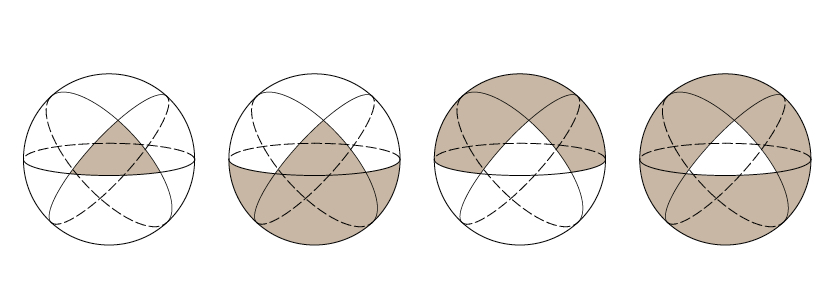
\includegraphics[width=0.9\textwidth]{kugel/Dreieckarten.jpg}
    \captionof{figure}{Dreiecksarten auf der Kugeloberfläche}
\end{center}

\subsection{Allgemeine Kugeldreiecke}

Ähnlich dem Dreieck in der Ebene hat das Dreieck auf der Kugel Seiten und Winkel. Allerdings werden die Seiten nicht in einer Länge angegeben sondern im Bogenmass. Auch hat das Dreieck auf der Kugel nicht zwingend $180^{\circ}$, die Winkelsumme liegt zwischen $180^{\circ}$ und zu $540^{\circ}$.

\subsection{Kugelzweieck}

Zwei Grosskreise auf der Kugeloberfläche zerlegen diese in vier gleich grosse Kugelzweiecke. 
Jedes dieser Dreieckseiten hat die Länge
$180^{\circ}$ oder $\pi$.
Der Flächeninhalt wird dabei nur durch den Winkel $\alpha$ zwischen den beiden Grosskreisen bestimmt.

\begin{center}
        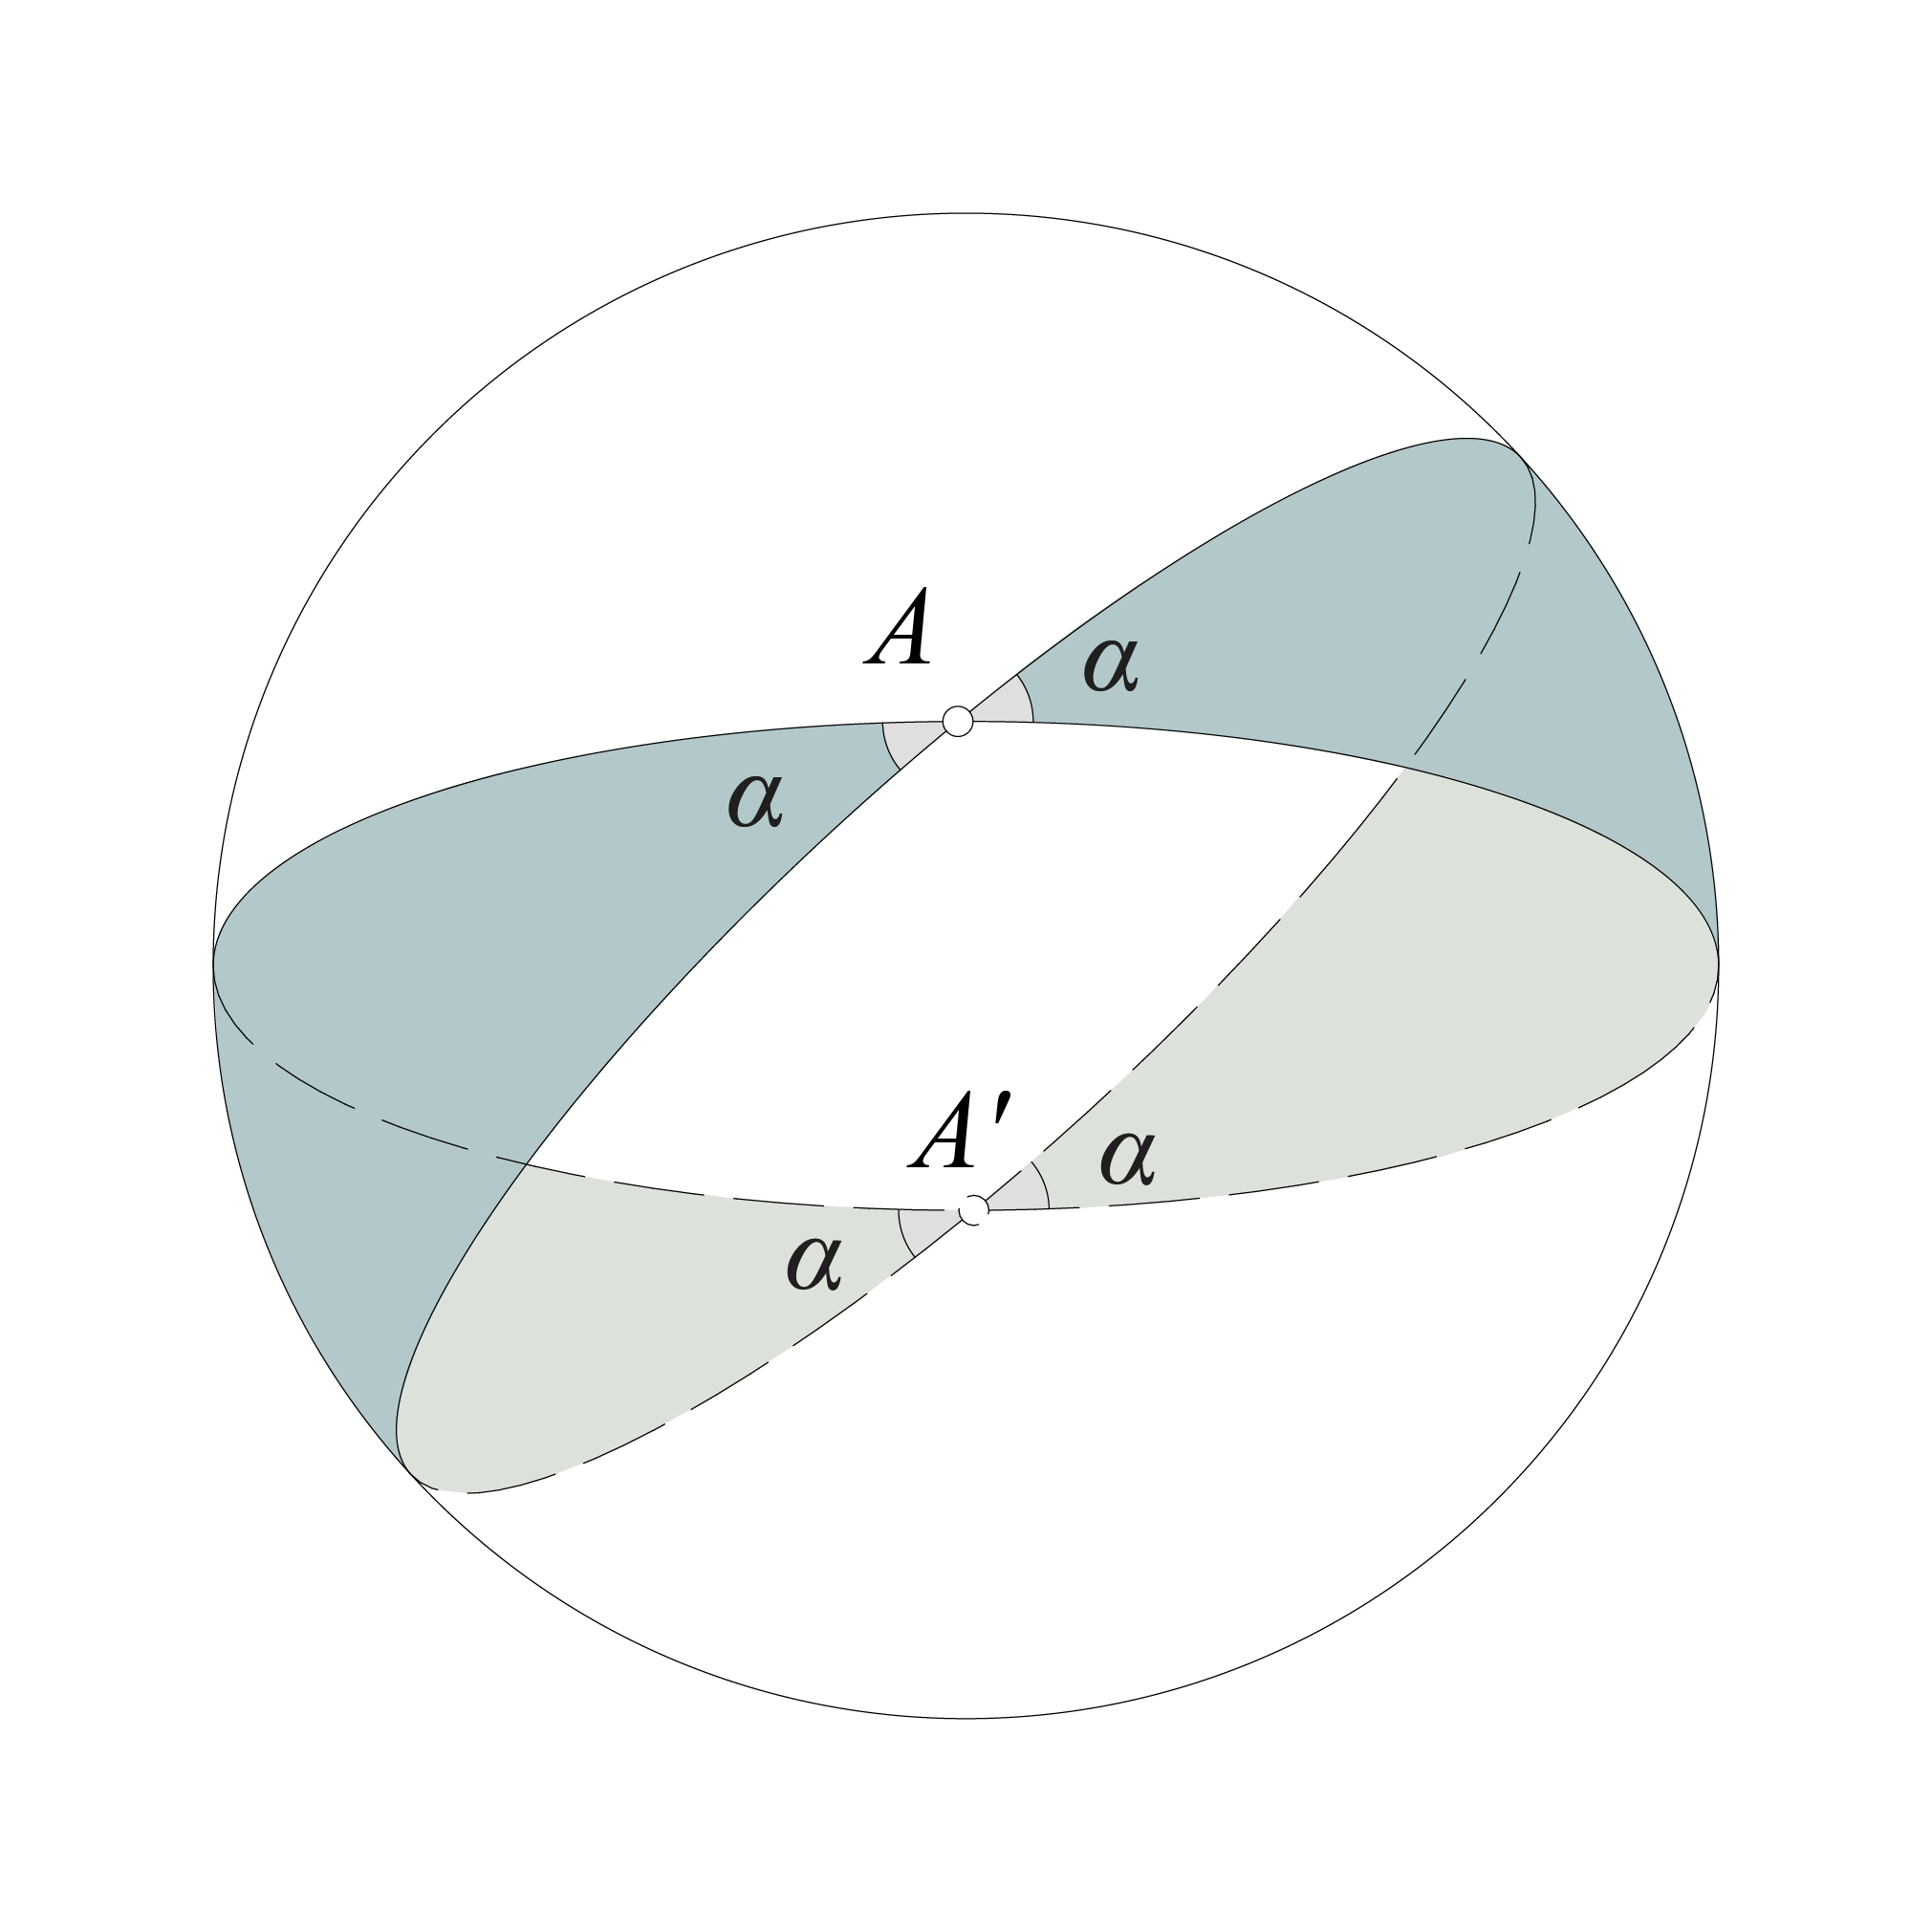
\includegraphics[width=0.3\textwidth]{kugel/Zweieck.jpg}
    \captionof{figure}{Bildung von Zweiecken durch Grosskreise}
\end{center}

Um den Flächeninhalt des Zweiecks zu erhalten, benötigen wir zuerst den Flächeninhalt der gesamten Kugel
\begin{align*}
A_{ Kugel } &= 4 \pi r^{2}
\end{align*}

Den Flächeninhalt der Kugel $A_{ Kugel }$ müssen wir noch mit dem Kugelsegment des Winkels $\alpha$ multiplizieren um dem Flächeninhalt des Zweiecks zu erhalten

\begin{equation}
A_{ Zweieck } = 4 \pi r^{2} \cdot \frac{ \alpha }{ 2 \pi }
\end{equation}

HIER NOCH EIN SATZ

\subsection{Eulersche’ Dreiecke}

Legt man drei Grosskreise auf eine Kugeloberfläche, bilden sich dabei acht Dreiecke. 
Ein solches Dreieck heisst Eulersches’Dreieck\footnote{%
Leonard Euler (1707-1783), berühmter Schweizer Mathematiker und Physiker. 
Nicht Eulersche’Dreiecke erhält man, indem man das Äussere des Dreieckes ABC betrachtet.}.
Diese Dreiecke werden weder durch die Verlängerung ihrer Seiten durchschnitten, 
noch haben sie Dreiecksseiten welche grösser als $180^{\circ}$ sind.

\begin{center}
        \includegraphics[width=0.4\textwidth]{kugel/Zweiecke.jpg}
    \captionof{figure}{Drei Grosskreise bilden ein sphärisches Dreieck}
\end{center}

In den nachstehenden Erklärungen und Herleitungen, sprechen wir ausschliesslich von Eulerschen’Dreiecken, da die umgeformten Winkelsätze der ebenen Trigonometrie nur auf diese Art von Kugeldreiecken angewendet werden kann.

$A_{ \overline{ ABC }}$ ist die Fläche des Dreieckes auf der Kugeloberfläche
In der ebenen Trigonometrie liegt die Winkelsumme eines Dreiecks bei
$180^{\circ}$.

Anders aber in der sphärischen Trigonometrie. Obschon sie einige Gemeinsamkeiten zur ebenen Trigonometrie aufweist, kann man nicht alles übernehmen.
So auch nicht wie Winkelsumme in einem sphärischen Dreieck.
Diese liegt bei:

\[
\begin{aligned}
\pi
&-
3\pi
&
&\text{\bigg \vert}
&
180^{\circ}
&-
540^{\circ}
\end{aligned}
\]

daraus lässt sich ableiten, das ein einzelner Winkel nicht grösser als $\pi$ oder $180^{\circ}$ sein darf. Ansonsten ist es kein Eulersches’Dreieck und wir dürfen die sphärische Trigonometrie nicht anwenden.\\
Wichtig anzumerken ist, dass die Seiten immer in Radiant beschrieben werden und nicht im Längenmass Meter wie wir es uns gewohnt sind. 
Bei den Dreiecksseiten handelt es sich um Kreisbögen und keine Strecken.

\section{Flächeninhalt sphärischer Dreiecke}

Der Flächeninhalt des Dreiecks $A_{ \triangle{ ABC }}$ berechnet sich aus den Winkeln $\alpha$, $\beta$, $\gamma$ und dem Kugelradius $r$ im Quadrat.
\begin{align*}
A_{ \triangle{ ABC }} &= (\alpha + \beta + \gamma) \cdot r^2
\end{align*}

\begin{center}
        \includegraphics[width=0.3\textwidth]{kugel/Beispielbild.jpg}
    \captionof{figure}{Bild FLäche dreieck}
\end{center}

Dies lässt sich folgendermassen herleiten: \\
Als erstes berechnen wir die Flächeninhalte der Zweiecke A, B und C

\begin{align*}
\text{Zweieck A}
&=
\triangle{ABC} + \triangle{A'BC} = 2 \alpha r^{ 2 } = A_{ \alpha }\\
\text{Zweieck B}
&=
\triangle{ABC} + \triangle{AB'C} = 2 \beta r^{ 2 } = A_{ \beta }\\
\text{Zweieck C}
&=
\triangle{ABC} + \triangle{ABC'} = 2 \gamma r^{ 2 } = A_{ \gamma }
\end{align*}

Addiert man nun die Flächeninhalte der einzelnen Zweiecke, ist diese Fläche gleich gross wie die der halben Kugel und zweimal des sphärischen Dreiecks $A_{ \triangle{ ABC }}$.

\begin{align*}
A_{ \alpha } + A_{ \beta } + A_{ \gamma } &= \frac{ 4\pi r^{ 2 } }{ 2 } + 2A_{ \triangle{ ABC }}
\end{align*}

Dies lässt sich umformen in

\begin{align*}
2\alpha r^{ 2 } + 2\beta r^{ 2 } + 2\gamma r^{ 2 } &= \frac{ 4\pi r^{ 2 } }{ 2 } + 2A_{ \triangle{ ABC }} \parallel:2
\end{align*}

Durch vereinfachen der Gleichung erhalten wir

\begin{align*}
\alpha r^{ 2 } + \beta r^{ 2 } + \gamma r^{ 2 } &= \pi r^{ 2 } + A_{ \triangle{ ABC }} \parallel-\pi r^{ 2 }\\
\end{align*}

Wir haben damit den folgenden Satz bewiesen:

\begin{satz}[\textit{Hallo ich heisse Flächeninhalt}]
\label{skript:kugel:satz:Flaecheninhalt}
\index{Flaecheninhalt}
\end{satz}

\begin{align*}
A_{ \triangle{ ABC }} &= r^{ 2 }\left(\alpha + \beta + \gamma - \pi\right) 
\end{align*}


\section{Sphärischer Exzess}
Anders als bei Dreiecken in der Ebene, ist die Winkelsumme bei sphärischen Dreiecken immer \textgreater \,  $\pi$.

\begin{align*}
\pi < \alpha + \beta + \gamma
\end{align*}

Der sphärische Exzess gibt dabei an, wie stark die Winkelsumme von $\pi$ abweicht.

\begin{align*}
\pi + \epsilon &= \alpha + \beta + \gamma \\
\end{align*}

Lösen wir nach $\epsilon$ auf:

\begin{equation}
\epsilon = \alpha + \beta + \gamma - \pi
\end{equation}

Zur Berechnung des Flächeninhalts eines sphärischen Dreiecks berechnet man demzufolge den sphärischen Exzess multipliziert mit dem Radius im Quadrat.
Dies zeigt, dass der Exzess direkt mit dem Flächeninhalt $A$ eines sphärischen Dreiecks zusammenhängt

\begin{align*}
\epsilon = \frac{A_{ \overline{ ABC }}}{r^2}
\end{align*}

\begin{center}
        \includegraphics[width=0.3\textwidth]{kugel/Beispielbild.jpg}
    \captionof{figure}{Bild Sphärischer Exzess}
\end{center}

Bei allgemeinen Kugeldreiecken gilt demnach:

\begin{align*}
\pi < \alpha + \beta + \gamma < 5\pi (900^{\circ})
\end{align*}


Bei Eulerschen’ Kugeldreiecken

\begin{align*}
\pi < \alpha + \beta + \gamma < 3\pi (540^{\circ})
\end{align*}

Der sphärische Exzess wird gleichmässig auf alle Winkel des Dreiecks aufgeteilt.

Bezieht man den sphärischen Exzess und die Formel des Flächeninhaltes auf die Erde und somit eine Kugel, kann man mit Hilfe eines beliebigen sphärischen Dreieckes und dessen Flächeninhalt auf den Radius der Kugel schliessen.

\subsection{Grenzfall - Satz von Legendre}

Würde der sphärische Exzess in der ebenen Trigonometrie angewendet, wäre dieser = 0.
Bei sehr kleinen sphärischen Dreiecken lässt sich dies annähernd wie in der ebenen Trigonometrie betrachten

\begin{quote} \textit{Ein kleines sphärisches Dreieck kann näherungsweise 
wie ein ebenes Dreieck mit denselben Seiten berechnet 
werden, wenn alle Winkel des ebenen Dreiecks die um 
je ein Drittel des sphärischen Exzesses verminderten 
Winkel des sphärischen Dreiecks nimmt.} \end{quote}
\begin{flushright} - Adrien-Marie Legendre (1752-1833), Paris 1787
\end{flushright}

Diese Aussage zeigt den Zusammenhang zwischen der 
Trigonometrie in der Ebene sowie in auf der Kugel
auf. Im speziellen bei sehr kleinen sphärischen 
Dreiecken ist die Winkelsumme nur unwesentlich 
grösser als $180^{\circ}$. 
Wichtig anzumerken ist, dass der Satz von Legendre 
für grosse, aber endliche Radien $r$ gilt.

\begin{center}
        \includegraphics[width=0.3\textwidth]{kugel/Beispielbild.jpg}
    \captionof{figure}{Bild Krümmung Gross und Klein}
\end{center}


\section{Sphärisch Analoge Winkelfunktionen}
Euklid von Alexandria\footnote{%
Euklid war ein griechischer Mathematiker. Er lebte wahrscheinlich 3 Jahrhunderte vor Christus. In seinem berühmtesten Werk \textit{Euklids Elemente} fasst er die Arithmetik und Geometrie seiner Zeit zusammen. \textit{Euklids Elemente} war 2000 Jahre lang als Lehrbuch in gebrauch und war bis Mitte des 19. Jahrhunderts nach der Bibel das weit verbreitetste Buch der Weltliteratur.}  beschrieb die Grundbegriffe der ebenen Geometrie mittels Punkt, Geraden, Ebene, Winkel und Dreieck. Ebendiese Dreiecke lassen sich mithilfe der ebenen Trigonometrie beschreiben. Dabei gelten die uns bekannten trigonometrischen Winkelfunktionen:\\

\text{Sinussatz:}
\begin{align*}
\frac{ a }{ sin(\alpha) } &= \frac{ b }{sin(\beta)} = \frac{ c }{ sin(\gamma) } = \frac{abc}{2A} = 2r\\
\end{align*}

\text{Cosinussatz:}
\begin{align*}
c^{ 2 } &= a^{ 2 } + b^{ 2 } - 2ab\cdot cos(\gamma)\\
b^{ 2 } &= a^{ 2 } + c^{ 2 } - 2ab\cdot cos(\beta)\\
a^{ 2 } &= b^{ 2 } + c^{ 2 } - 2ab\cdot cos(\alpha)
\end{align*}

Um diese Winkelfunktionen auf der Kugeloberfläche anwenden zu können, benötigen wir die sphärische Trigonometrie. Die oben beschriebenen Sätze lassen sich auf der Kugel nicht anwenden, sie werden aber als Grundlage und Gedankenstütze zur Herleitung der Sätze für das Kugeldreieck benötigt.

\subsection{Sphärischer Sinussatz}

\begin{center}
        \includegraphics[width=0.3\textwidth]{kugel/Beispielbild.jpg}
    \captionof{figure}{Bild Sinussatz}
\end{center}


Wir betrachten das folgende sphärische Dreieck auf einem Teilstück der Kugeloberfläche mit dem Radius $R= \overline{MA} = \overline{MB} = \overline{MC}$. Danach fügen wir ein ebenes Dreieck $\triangle=\overline{ADE}$ in das Kugelstück ein, welches den Eckpunkt $A$ des sphärischen Dreiecks beinhaltet und eine Abbildung des sphärischen Dreieckes bildet.

Es gilt

\begin{align*}
\overline{AD} &= R \cdot sin (c) \\
hA = \overline{AF} &= \overline{AD} \cdot sin(\beta) = R \cdot sin(c) \cdot sin(\beta)  
\end{align*}

Aus einer anderen Sichtweise kann man auch schreiben

\begin{align*}
h_{A} = R \cdot sin(b) \cdot sin(\gamma)  
\end{align*}

Durch gleichsetzen dieser Ausdrücke ergibt sich

\begin{align*}
R \cdot sin(c) \cdot sin(\beta) &= R \cdot sin(b) \cdot sin(\gamma) \\
\Rightarrow \quad \quad
sin(c) \cdot sin(\beta) &= sin(b) \cdot sin(\gamma) \\
\Rightarrow \quad \quad
\frac{sin (b)}{sin (c)} &= \frac{sin (\beta)}{sin (\gamma)}
\end{align*}

Analog dazu könnte man auch die Höhe $h_{B}$ nehmen und würde erhalten

\begin{align*}
sin(c) \cdot sin(\alpha) &= sin(a) \cdot sin(\gamma) \\
\Rightarrow \quad \quad
\frac{sin (a)}{sin (c)} &= \frac{sin (\alpha)}{sin (\gamma)}
\end{align*}

Aus diesen Erkenntnissen lässt sich der Sinussatz zusammenfassen

\begin{satz}[\textit{Der sphärische Sinussatz verhaltet sich wie der Sinus der Seiten wie der Sinus der Gegenwinkel, dies lässt sich beschreiben}]
\label{skript:kugel:satz:Sinussatz}
\index{Sinussatz}
\end{satz}

\begin{align*}
\sin(a) : \sin(b) : \sin(c) &= \sin(\alpha) : \sin(\beta) : \sin(\gamma) \\
 \\
\frac{sin(\alpha)}{sin(a)} &= \frac{sin(\beta)}{sin(b)} = \frac{sin(\gamma)}{sin(c)}
\end{align*} 


\subsection{Seitenkosinussatz}

Es sei das Stück einer Kugel mit dem sphärischen Dreieck $ABC$ und den Winkeln $\alpha, \beta, \gamma$ und den Seiten $a, b, c$. Die Senkrechten durch den Mittelpunkt, schneiden dabei die Eckpunkte des sphärischen Dreieckes. Wir erstellen in der Ebene ein Ähnliches Dreieck $A’B’C’$.

\begin{center}
        \includegraphics[width=0.3\textwidth]{kugel/Beispielbild.jpg}
    \captionof{figure}{Bild Seitenkosinus}
\end{center}

Dabei lassen sich die Strecken nach den uns bekannten Regeln der Trigonometrie beschreiben:

\begin{align*}
\overline{C'A'} &= d\cdot {tan(b)} \\
\overline{C'B'} &= d\cdot {tan(a)} \\
\overline{MA'} &= \frac{ d }{cos(b)} \\
\overline{MB'} &= \frac{ d }{cos(a)}
\end{align*} 

Dabei schreibt sich der Kosinussatz der Ebene wie folgt

\begin{align*}
c^{ 2 } &= a^{ 2 } + b^{ 2 } - 2ab \cdot cos(\gamma)
\end{align*}

Daher gilt für das Dreieck $A’B’C’$

\begin{align*}
\triangle \overline{A'B'}^{ 2 } &= \overline{ C'B' }^{ 2 } + \overline{ C'A' }^{ 2 } - 2 \cdot \overline{C'B'} \cdot \overline{ C'A' } \cdot cos(\gamma) \\
\Rightarrow \quad \quad
\triangle \overline{A'B'}^{ 2 } &= d^{ 2 } \cdot \left(\left(tan^{ 2 }(a) + tan^{ 2 }(b)\right) - 2\cdot tan(a) \cdot tan(b) \cdot cos(\gamma)\right)
\end{align*}


das gilt ebenso für das Dreieck $MA’B’$

\begin{align*}
\triangle \overline{ MA'B' }^{ 2 } &= \overline{ MB' }^{ 2 } + \overline{ MA' }^{ 2 } - 2\cdot \overline{ MB'} \cdot \overline{ MA' } \cdot cos(c) \\
\Rightarrow \quad \quad
\overline{ MA'B'}^{ 2 } &= \left(\frac{ d }{ cos(a) }  \right)^{ 2 } + \left(\frac{ d }{ cos(b)}  \right)^{ 2 } - 2 \cdot \frac{ d }{ cos(a)} \cdot \frac{ d }{ cos(b)} \cdot cos(c)
\end{align*}


Im Einheitskreis betrachtet ergibt dies

\begin{align*}
\overline{ MA'B' }^{ 2 } &= d^{ 2 } \cdot \left(\left(\frac{ 1 }{ cos(a) }  \right)^{ 2 } + \left(\frac{ 1 }{ cos(b) }  \right)^{ 2 } - 2 \cdot \frac{ 1 }{ cos(a)} \cdot \frac{ 1 }{ cos(b)} \cdot cos(c)\right)
\end{align*}


Durch berücksichtigen von $\frac{1}{\cos^{2}(x)}=\tan^{2}(x)+1$ folgt

\begin{align*}
\overline{ A'B'}^{ 2 } &= d^{ 2 } \cdot \left(\left(tan^{ 2 }(a) + tan^{ 2 }(b)\right) - 2 \cdot \frac{ 1 }{ cos(a)} \cdot \frac{ 1 }{ cos(b)} \cdot cos(c)\right) \\
\Rightarrow \quad \quad
\overline{ A'B'}^{ 2 } &= d^{ 2 } \cdot \left(\left(tan^{ 2 }(a) + 1\right) + \left(tan^{ 2 }(b) + 1\right) - \left(2 \cdot \frac{cos(c)}{cos(a) \cdot cos(b)}\right)\right)
\end{align*}


Durch gleichsetzen dieser beiden Ausdrücke folgt

\begin{align*}
2 \cdot tan(a) \cdot tan(b) \cdot cos(\gamma) &= -2+2 \cdot \frac{cos(c)}{cos(a) \cdot cos(b)}
\end{align*}

Durch umformen durch $\tan(a)=\frac{\sin(a)}{\cos(a)}$ und der Multiplikation mit  $\frac{1}{2}$ ergibt sich

\begin{align*}
\frac{\sin(a)}{\cos(a)} \cdot \frac{\sin(b)}{\cos(b)} \cdot \cos(\gamma) &= -1 + \frac{\cos(c)}{\cos(a) \cdot \cos(b)}
\end{align*}

Durch vereinfachen der Formel erhalten wir den Seitenkosinussatz der Seite $c$

\begin{align*}
\cos(a) \cdot \cos(b) + \sin(a) \cdot sin(b) \cdot \cos(\gamma) = \cos(c)
\end{align*}

Durch zyklische Vertauschung der Variablen erhält man den 

\begin{satz}[\textit{Im sphärischen Dreieck ist der Kosinus einer Seite gleich der Summe der Kosinusprodukte der beiden anderen Seiten und dem mit dem Kosinus des eingeschlossenen Winkels multiplizierten Sinusprodukt dieser Seiten}]
\label{skript:kugel:satz:Seitenkosinussatz}
\index{Seitenkosinussatz}
\end{satz}


\begin{align*}
{\cos a} &= {cos(b)} \cdot {cos(c)} + {sin(b)} \cdot {sin(c)} \cdot {cos(\alpha)}\\
{cos(b)} &= {cos(c)} \cdot {cos(a)} + {sin (c)} \cdot {sin(a)} \cdot {cos(\beta)}\\
{cos(c)} &= {cos(a)} \cdot {cos(b)} + {sin(a)} \cdot {sin(b)} \cdot {cos(\gamma)}\\
\end{align*}


ABSCHLUSSATZ

\subsection{Winkelkosinussatz}

Wenden wir den sphärischen Seitenkosinussatz auf dem Polardreieck an, erhalten wir
\begin{align*}
{\cos (a)} = {\cos (b)} \cdot {\cos (c)} + {\sin(b)} \cdot {\sin(c)} \cdot {\cos (\alpha)}
\end{align*}

\begin{center}
        \includegraphics[width=0.3\textwidth]{kugel/Beispielbild.jpg}
    \captionof{figure}{Bild Winkelkosinus/Polardreieck}
\end{center}

Durch die Beziehung zwischen dem Polardreieck und einem sphärischen Dreieck, können wir den Seitenkosinussatz folgendermassen umformen
\begin{align*}
{\cos (\pi-\alpha)} &= {\cos (\pi-\beta)} \cdot {\cos (\pi-\gamma)} + {\sin(\pi-\beta)} \cdot {\sin(\pi-\gamma)} \cdot {\cos (\pi-a)}
\end{align*}

Durch die Quadrantenbeziehung der trigonometrischen Funktionen im Einheitskreis folgt

\begin{align*}
\sin (\pi-\alpha) &= sin(\alpha)\\
\cos (\pi-\alpha) &= - cos (\alpha)\\
\end{align*}

Daher ergibt sich

\begin{align*}
{-\cos (\alpha)} &= {-\cos (\beta)} \cdot {-\cos (\gamma)} + {\sin(\beta)} \cdot {\sin(\gamma)} \cdot {-\cos (a)}
\end{align*}

Durch vertauschen der Vorzeichen erhalten wir den Winkelkosinussatz

\begin{satz}[\textit{Im sphärischen Dreieck ist der Kosinus eines Winkels gleich der Summe aus dem negativen Produkt der Kosinus der beiden anderen Winkel und dem mit dem Kosinus der gegenüberliegenden Seite multiplizierten Sinusprodukt der beiden anderen Winkel.}]
\label{skript:kugel:satz:Winkelkosinussatz}
\index{Winkelkosinussatz}
\end{satz}

\begin{align*}
{\cos (\alpha)} &= {-\cos(\beta)} \cdot {\cos(\gamma)} + {\sin (\beta)} \cdot {\sin(\gamma)} \cdot {\cos(a)}\\
{\cos (\beta)} &= {-\cos(\gamma)} \cdot {\cos(\alpha)} + {\sin (\gamma)} \cdot {\sin(\alpha)} \cdot {\cos(b)}\\
{\cos (\gamma)} &= {-\cos(\alpha)} \cdot {\cos(\beta)} + {\sin (\alpha)} \cdot {\sin(\beta)} \cdot {\cos(c)}\\
\end{align*}

ABSCHLUSSATZ

\section{Dualität auf der Kugel}

Durch die Herleitung des Winkelkosinussatzes haben wir zugleich die Dualität auf der Kugel bewiesen.

\begin{satz}[\textit{Die sphärische Geometrie ist eine projektive Geometrie. In der projektiven Geometrie lassen sich alle Sätze dualisieren, das heisst, die Begriffe Punkt und Geraden werden vertauscht; demzufolge auch Längen und Winkeln}]
\label{skript:kugel:satz:Dualitaet}
\index{Dualitaet}
\end{satz}

\begin{center}
        \includegraphics[width=0.3\textwidth]{kugel/Beispielbild.jpg}
    \captionof{figure}{Bild Dualität}
\end{center}

Dualisiert man nun als Beispiel einen Punkt und eine Gerade, bleibt die Beziehung zwischen dem Punkt und der Geraden erhalten.
Nimmt man nun den Punkt $A$ welcher auf der Geraden $b$ liegt, so verläuft die Duale Gerade $a$ durch den zur Geraden $b$ dualen Punkt $B$. 
Aber nicht nur die Beziehungen zwischen Punkten und Längen bleiben erhalten. Auch die Winkel und Längen gehen ineinander über wie wir es im Beweis des Winkelkosinussatzes gesehen haben.
Der Winkel $\gamma$ zwischen den beiden Seiten a und b entspricht auf der Einheitskugel dem Abstand zwischen den zu der Geraden dualen Punkten A und B.

\section{Navigation auf See}
Das besondere an Seekarten ist die Inhaltliche Ausrichtung. Anders wie Landkarten muss sie Informationen enthalten welche für den Kapitän und seine Besatzung von grosser Bedeutung sind. Vor allem in Küstennähe ist das navigieren eines Schiffes besonders gefährlich. So enthalten Seekarten etwas über Wassertiefen, Bodenbeschaffenheiten, Gezeiten, Küstenlinien, Landzungen und Windrichtungen.
Der Hauptunterschied dabei ist, das auf der Landkarte feste Positionen definiert und aufgezeigt werden, das einzige was sich verändert ist der Reisende selbst. Bei der Seekarte ist das anders, es werden veränderliche Einwirkungen der Natur festgehalten.

Dieser kleine Unterschied zeigt die Notwendigkeit auf, die Position und den Kurs seines Schiffes auf See immer ermitteln zu können.


\section{Geographische Koordinaten}

Nachdem klar war, das die Erde eine Kugel ist, wurde diese in ein Gradnetz aufgeteilt. Dabei wurden die Angaben für eine exakte Ortsbestimmung klar definiert und die bis heute gültigen Koordinaten bestimmt.
Dabei muss man sich nochmals in Erinnerung rufen, dass sich die Erde in 24h einmal um ihre eigene Achse dreht. Nach $360 ^{\circ}$ 
und somit einer vollen Umdrehung, steht sie wieder in ihrer Ursprungsposition und ein neuer Tag beginnt.

Die Koordinaten setzen sich aus folgenden Komponenten zusammen:

\[
\begin{aligned}
&\text{Grad } (^{\circ})
&
&\text{\bigg \vert}
&
&\text{Bogenminuten } (`)
&
&\text{\bigg \vert}
&
&\text{Bogensekunden } (``)
\end{aligned}
\]

Die Erdoberfläche wurde in je 360 Breiten- und Längengrade eingeteilt. Die Breitengrade haben zueinander einen Abstand von 111.31 km, dies entspricht auch dem Abstand der Längengrade am Äquator mit Zunehmender Nähe zu den Polen, nimmt dieser Abstand ab.

\[
\begin{aligned}
&1^{\circ}
&
&\text{\bigg \vert}
&
&4 \text{ Minuten}
&
&\text{\bigg \vert}
&
&111.31\text{ km}
\end{aligned}
\]

Berechnet man nun die Erdumdrehung von 360°, erhält man genau den Erdumfang am Äquator: \begin{align*} 40’074 \text{ km.}\end{align*}

Dabei geben die Bogenminuten und -sekunden dem Standort die gewünschte Exaktheit. Mit den vollständigen Koordinaten lässt sich der Standort auf einer Landkarte exakt bestimmen und einzeichnen.

\subsection{Erdachsenneigung}

Die Erdachse oder auch Rotationsachse der Erde ist um ca. $23.5^{\circ}$ geneigt.
Dadurch lassen sich Phänomene wie die vier Jahreszeiten sowie die unterschiedliche Längen der einzelnen Tage herleiten.
Für die nautische Navigation hat dies eine grosse Bedeutung, da je nach Neigung andere Sterne zu sehen sind, auch die Sonne ist an einem anderen Ort am Himmel zu finden.

\begin{center}
        \includegraphics[width=0.3\textwidth]{kugel/Beispielbild.jpg}
    \captionof{figure}{Bild Erdneigung}
\end{center}

Der Himmelsäquator ist die Linie, die orthogonal zur Sonne verläuft.
Die Ekliptil-Linie ist die Linie, die orthogonal zur Erdachse verläuft.
Der Schnittpunkt dieser Kreise wird als Frühlings- / Herbstpunkt bezeichnet und ist jeweils am 21. März / 21. Oktober des Jahres.
Der Frühlingspunkt $\Upsilon$ wird oft als Gestirnspunkt im nautischen Dreieck verwendet, genaueres wird im Kapitel zum nautischen Dreieck erklärt.


\subsection{Zeitzonen der Erde}
Wenn man nun die verschiedenen Zeitzonen der Erde betrachtet, macht die Verschiebung von jeweils einer Stunde durchaus Sinn, es lässt sich auf die Längengrade schliessen.
Zwischen den verschiedenen Zeitzonen liegen 15 Längengrade:
\begin{align*}
\text{15 Längengrade à 4 Minuten = 60 Minuten Zeitverschiebung = ca. 1665 km}
\end{align*}

Dabei ist die Zeitzone in welcher Mitte sich der Greenwich Meredian befindet die \textit{Greenwich Mean Time (GMT)} welche bis 1928 als Weltzeit galt. Im Jahr 1972 wurde diese umbenannt in die \textit{Coordinated Universal Time (UTC)} und wir von da an als Weltzeit $\pm$ 0.00 verwendet.


\section{Der Breitengrad}
Die Breitengrade bilden die bereits genannten Kleinkreise auf der Kugeloberfläche. Sie verlaufen in einem Abstand von genau 111 km parallel zum Äquator. Dabei stellt  dieser genau die Mitte zwischen Nord- und Südpol dar und teilt die Erdkugel in zwei gleiche Hälften. Somit wird von nördlicher und südlicher Breite gesprochen, je nach dem auf welcher Halbkugel man sich befindet.

\begin{center}
        \includegraphics[width=0.3\textwidth]{kugel/Beispielbild.jpg}
    \captionof{figure}{BILD SKIZZE DER GEOGRAFISCHEN BREITE ERDKUGEL}
\end{center}


\subsection{Geografische Breite $\phi$}
\begin{definition}
Die geografische Breite eines Standortes ist nichts anderes, als der Winkel am Erdmittelpunkt zwischen der Ebene des Äquators und der Geraden zum Standpunkt auf der Erdoberfläche.
\end{definition}

\begin{center}
        \includegraphics[width=0.3\textwidth]{kugel/Beispielbild.jpg}
    \captionof{figure}{Bild}
\end{center}


\subsection{Navigation mit den Breitengraden}
Da der Breitengrad bereits sehr früh ziemlich präzise bestimmt werden könnte, nutzten bereits die Seefahrer um Christoph Kolumbus den Breitengrad zur Navigation ihrer Flotten.
Den dieser lässt sich ziemlich einfach aus dem höchsten Sonnenstand oder einem Fixstern bestimmen. Dabei wird mit einem Jakobsstab\footnote{%
Der Jakobsstab ist ein früheres astronomisches Instrument zur Winkelmessung und wurde vor allem in der Seefahrt verwendet. Er ist in der Nautik der Vorläufer des Sextanten.} (später Sextant\footnote{%
Der Sextant ist ein nautisches Messinstrument zur Winkelmessung von Horizont und Fixstern (Gestirn)}) der Winkel zwischen dem Horizont und dem Fixstern gemessen. Der Winkel welchen man erhält, zieht man von 90° ab und erhält somit die geografische Breite. \\

\begin{center}
        \includegraphics[width=0.3\textwidth]{kugel/Beispielbild.jpg}
    \captionof{figure}{Bild}
\end{center}

Wenn man sich auf der Nordhalbkugel befindet, ist der Polarstern ein sehr guter Fixstern. Befindet sich ein Schiff nun sehr nahe am Nordpol, steht dieser nahezu senkrecht am Himmelszelt bei $90^{\circ}$. Würde es aber nahe dem Äquator stehen, erscheint dieser am Horizont bei $0^{\circ}$.

\subsection{Korrekturbeiwert}
Die Breitengrade auf der Erde haben nicht alle den selben Radius. Daher segelt man am Äquator viel länger dem Breitengrad entlang um zum nächsten Längengrad zu kommen wie in der nähe des Nord- oder Südpols.

\[
\begin{aligned}
&\text{1} (^{\circ})
&
&\text{\bigg \vert}
&
&\text{4 Minuten}
&
&\text{\bigg \vert}
&
&\text{111.13 km}
\end{aligned}
\]

\[
\begin{aligned}
&\text{0.25} (^{\circ})
&
&\text{\bigg \vert}
&
&\text{1 Minute}
&
&\text{\bigg \vert}
&
&\text{27.78 km}
\end{aligned}
\]

\[
\begin{aligned}
&\text{0.004166} (^{\circ})
&
&\text{\bigg \vert}
&
&\text{1 Sekunde}
&
&\text{\bigg \vert}
&
&\text{463m}
\end{aligned}
\]

Um die Minderung der Strecke zu erhalten, müssen wir den Cosinus des gemessenen Breitengrades berechnen und diesen mit der Abweichung auf dem Äquator von 1 Sekunde multiplizieren.

\begin{center}
        \includegraphics[width=0.3\textwidth]{kugel/Beispielbild.jpg}
    \captionof{figure}{Bild}
\end{center}

\[
\begin{aligned}
&\cos 90^\circ \cdot 463m = 463m
&
&\text{\bigg \vert}
&
&\cos 50^\circ \cdot 463m = 297.61m
&
&\text{\bigg \vert}
&
&\cos 0^\circ \cdot 463m = 0m
\end{aligned}
\]

Dies zeigt auf je näher man den Polen ist, desto weniger weit muss man Segeln um den nächsten Längengrad zu erreichen.

\section{Der Längengrad}
Die Längengrade bilden die bereits genannten Grosskreise auf der Kugeloberfläche.
Sie schneiden den Äquator im rechten Winkel, haben dort einen Abstand von 111 km zueinander und verbinden die Pole. Anders wie bei der geografischen Breite, ist in der Natur kein Längengrad gegeben welcher den Nullpunkt darstellt.

\begin{center}
        \includegraphics[width=0.3\textwidth]{kugel/Beispielbild.jpg}
    \captionof{figure}{Bild}
\end{center}


\subsection{Geografische Länge $\lambda$}
\begin{definition}
Die geografische Länge ist der Winkel an der Erdachse zum Nullmeridian.
\end{definition}

\subsection{Navigation mit den Längengraden}
Die geografische Länge lässt sich nicht so einfach bestimmen wie deren Breite. Für die Berechnung auf See benötigt man eine Referenzzeit eines Ortes mit bekannter Länge.
In der Zeit der Entdecker gab es noch keine mechanischen Uhren. Die Sonnenuhr war zudem ungeeignet, da diese nur die Uhrzeit am Standort mass und nicht die am Referenzort selbst. Die erste Pendeluhr wurde erst Mitte des 17. Jahrhunderts erfunden, was in der Schifffahrt aber auch nicht die Lösung brachte.\\
Pendeluhren auf einem Schiff sind ungeeignet, da das Pendel mit dem Wellengang aus dem Takt gebracht wird und somit die Uhr falsch geht.
Zu ungenau und gegen äussere Erschütterungen zu empfindlich waren später auch die federgetriebenen Uhren und die Unruh. Dazukamen die verschiedenen Klimazonen welche ein Schiff zu durchqueren hatten. Das Metall zog sich viel zu fest zusammen oder dehnte sich aus, was dazu führte das die Uhr unregelmässig lief.

Das sogenannte „Längenproblem“ stellte nicht nur bei der Navigation auf See ein Problem dar, es ergaben sich auch wirtschaftliche Konsequenzen. Die Schiffe mussten bis zur gewünschten geografischen Breite navigieren und segelten dann den Breitengrad entlang. Dabei waren die Schiffe oft Wochenlang unterwegs und segelten die „Breiten ab“ um an die gewünschte Position zu kommen. Dies führte zu erheblichen Zeitverlusten und viel längeren Reisezeiten.


\section{The Board of Longitude - Das Längenproblem}
Das Längenproblem beschäftigte alle grossen Seefahrernationen Europas. Die fehlenden Längengrade bei der Navigation führten zu vielen Schiffsunglücken. Dies zeigt auch die Dringlichkeit der Lösung dieses Problems auf: Nicht selten kam es vor, das sich auf den verloren gegangenen Schiffen Schätze in der Höhe von halben britischen Staatshaushalten befanden. Der Verlust solcher Schiffe war enorm.\\
Bereits um 1600 hatte der König von Spanien ein Preisgeld ausgeschrieben für denjenigen welcher eine Lösung für das Problem präsentieren konnte. Leider ohne Erfolg. \\

Nach einem tragischen Unglück im Jahr 1707 beidem der siegreiche Admiral Sir Cloudesley und seine 1’450 Mann sein Leben liessen, indem sie auf die Scilly-Inseln kurz vor Land’s End aufliefen und dabei die 21 Schiffe sanken, rückte das Problem wieder in den Vordergrund.
114 Jahre später, nach einer Petition von William Whiston und Humphry Ditton welche von Sir Isaac Newton und Edmond Halley untermauert wurde, reagierte das britische Parlament.
Es schrieb folgende Preisgelder für eine praktisch, brauchbare Lösung aus:\\

\begin{compactitem}
\item £ 20’000 - Abweichung von max. $\frac{1}{2}^{\circ}$
\item £ 15’000 - Abweichung von $\frac{2}{3}^{\circ}$
\item £ 10’000 - Abweichung von max. $1 ^{\circ}$
\end{compactitem}
\\
Im Kapitel der Korrekturbeiwertberechnung des Breitengrades haben wir erfahren, das eine Abweichung von $1 ^{\circ}$ am Äquator ca. 111km entsprechen - dies sind 60 Seemeilen.
Auf der Höhe des Ärmelkanals und damit London, beträgt die Abweichung nur noch 74km und somit 40 Seemeilen.//
Das Preisgeld entsprach einer enorm hohen Summe für diese Zeit. Der Kaufpreis für ein mittleres Schiff welches zur See fahren konnte lag bei etwa 1’500-2’500£, ein einzelner Arbeiter lebte mit 10£ im Jahr.
Würde man dieses Problem heute mit einer Abweichung von einem halben Grad lösen, erhielte man 2’840’000£ was etwa einem Wert von 3’600’000 Schweizer Franken entspräche. \\

Damit die Lösungsvorschläge kontrolliert und verwaltet werden konnten, wurde die Board of Longitude (Längenkommission) gegründet. Ihr gehörten die bedeutendsten Astronomen und Mathematiker dieser Zeit an, aber auch d



\subsection{John Harrison}

\begin{center}
        \includegraphics[width=0.3\textwidth]{kugel/JohnHarrison.jpg}
    \captionof{figure}{Bild John Harrison}
\end{center}





\begin{center}
        \includegraphics[width=0.2\textwidth]{kugel/HarrisonH4.jpg}
    \captionof{figure}{Bild Harrison's H4}
\end{center}


\subsection{Tobias Mayer}

\begin{center}
        \includegraphics[width=0.3\textwidth]{kugel/TobiasMayer.jpg}
    \captionof{figure}{Bild}
\end{center}

Tobias Mayers\footnote{%
Tobias Mayer (1723-1762) studierte nie an einer Universität und war trotzdem ein annerkannter Wissenschaftler seiner Zeit in den Bereichen Astronomie, Geo- und Kartograf, Mathematiker und Physiker.} 
 Mondkarten galten ein halbes Jahrhundertlang als unübertroffen. Der Ruhm galt aber hauptsächlich seinen Mondkarten welche er im Jahr 1755 in einer erweiterten Version dem britischen Parlament vorlegte.\\
Mit ihnen konnte man die Geografische Länge bis auf 5 Bogensekunden genau bestimmen. Dies entsprach am Äquator $0.5 ^{\circ}$, was wiederum eine Genauigkeit von 55.565km entsprach.\\
Eine Lösung für das Längenproblem war gefunden. Die Publikation seiner Mondtafeln fand 1767 unter dem Titel \textit{Theoria lunae juxta systema Newtonianum} in London statt, 5 Jahre nach Mayers Tod. 
Seine Witwe schickte die publizierten Mondkarten über die Universität Göttingen nach Grossbritannien. Sie erhielt von der britischen Regierung eine Prämie in der Höhe von £ 3’000.-.

Im Jahr 1935 wurde ein Krater auf der westlichen Mondvorderseite nach dem deutschen Astronomen benannt, er trägt fortan den Namen T.Mayer.

\begin{center}
        \includegraphics[width=0.3\textwidth]{kugel/Mondkarte.jpg}
    \captionof{figure}{Mondkarte}
\end{center}


\section{Nautisches oder Astronomisches Dreieck}
Ein sphärisches Dreieck an der Himmelskugel welches folgende Eckpunkte hat
- Zenit
- Himmelsnordpol
- Gestirn
nennt man nautisches Dreieck.\\

Es ist ein Hilfsmittel wenn es darum geht, den Standort seines Beobachtungspunktes auf dem offenen Meer herauszufinden oder den Standort eines Sterns zum bestimmten Zeitpunkt zu ermitteln.

\subsection{Das Horizontsystem (lokale Beobachtung)}


\subsubsection{Gestirnshöhe $h$}
Ist die sphärische Entfernung des Gestirns vom Horizont, gezählt nordwärts $+0^{\circ}$ bis $+90^{\circ}$ und südwärts $-0^{\circ}$ bis $-90^{\circ}$.

\subsubsection{Azimut $a$}
Bogen zwischen dem Ortsmeridian und denm Höhenkreis des Gestirns, gezählt auf dem Höhenkreis vom Südpunkt aus über Westen $+0^{\circ}$ bis $360^{\circ}$.



\subsection{Das Äquatorsystem (astronomische Jahrbücher)}


Um die Anwendung des nautischen Dreiecks aufzeigen zu können, benötigt es ein Grundwissen der astronomischen Begriffe in der Navigation.


\subsubsection{Stundenwinkel $\tau$}
Der Winkel zwischen dem Deklinationswinkel und Ortsmeridianm gezählt auf dem Himmelsäquator vom in Ortsmeridian in Richtung SWNO vom höchsten Stand des Gestirns, gemessen $+0^{\circ}$ bis $+360^{\circ}$.


\subsubsection{Deklination $\delta$}
Der sphärische Abstand des Gestirns vom Äquator, gezählt am Deklinationskreis nordwärts von $+0^{\circ}$ bis $+90^{\circ}$ und südwärts $-0^{\circ}$ bis $-90^{\circ}$.

\subsu









bsection{Ekliptik}
Ist die scheinbare jährliche Sonnenbahn. Sie besitzt gegen den Äquator eine Neigung von $\epsilon$ = $23^{\circ}$ 27'. Der Schnittpunkt mit der Ekliptik werden Frühlingspunkt $\Upsilon$ und Herbstpunkt genannt. 

%GRAFIK ÄQUATOR UND HORIZONTALWENDEKREIS

\subsubsection{Rektaszension $\alpha$}
Bogen auf Äquator, gezählt vom Frühlingspunkt $\Upsilon$ aus entgegengesetzte dem Sinne der täglichen Sonnenbewegung von $+0^{\circ}$ bis $+360^{\circ}$.

\subsubsection{Ekliptikale Länge $\lambda$}
Bogen und Ekliptik zwischen Frühlingspunkt $\Upsilon$ und Breitenkreis, gezählt vom Frühlingspunkt aus entgegengesetzt dem Sinne der täglichen Sonnenbewegung von $+0^{\circ}$ bis $+360^{\circ}$.

\subsubsection{Ekliptikale Breite $\beta$}
Sphärischer Abstand des Gestirns von der Ekliptik, gezählt von der Ekliptik aus nordwärts von $+0^{\circ}$ bis $+90^{\circ}$ und südwärts von $-0^{\circ}$ bis $-90^{\circ}$.

\subsubsection{Kulmination}
Durchlaufen des höchsten und tiefsten Punktes der täglichen Bahn eines Gestirnes.


\subsection{Anwendung}





\begin{center}
        \includegraphics[width=0.3\textwidth]{kugel/Beispielbild.jpg}
    \captionof{figure}{Bild}
\end{center}





\section{Die Vermessung der Welt}
Wir schreiben das Jahr 1818 und kehren in die Zeit des Mathematikers Carl Friedrich Gauss zurück. Neben dem liebevoll genannten „kleinen Gauss“ und anderen herausragenden Mathematischen Leistungen, beschäftigte er in den Folgejahren mit der Vermessung des Königreichs Hannovers und verfasste auf 61 Blättern das Kartenwerk \textit{Gauss’sche Landesaufnahme der 1815 durch Hannover erworbenen Gebiete}.
\cite{skript:tabea}


$\Rightarrow$
Hubble Teleskop 
24. April 1990


\chapter{Geometrie auf der Kugeloberfläche\label{chapter:kugel}}
\lhead{Geometrie auf der Kugeloberfläche}
\begin{refsection}
\chapterauthor{Melina Staub und Fabian Schmid}

\section{Einleitung}

Seit jeher fasziniert den Menschen die Fahrt zur See. Nicht grundlos ist die Seefahrt eine der wichtigsten und ältesten Tätigkeiten der Menschheit. Der innerliche Drang neue Weltmeere und unbekannte Gebiete zu entdecken, die Fahrt zur See zu erleichtern und erträglicher zu machen, trieben die Menschen an, die Schiffe dieser Welt immer weiter zu entwickeln.

Die Idee der Kugelform der Erde ist älter als man zu denken vermag. Bereits der Schüler des antiken griechischen Philosophen Platon - Aristoteles schrieb in seiner Schrift \textit{Über den Himmel} aus dem 4. Jahrhundert v. Chr. etliche Gründe welche für die Gestallt der Erde als Kugel sprechen:\\

\begin{compactitem}
      \item Sämtliche schweren Körper streben zum Mittelpunkt des Alls. Da sie dies von allen Seiten her gleichmässig tun und die Erde im Mittelpunkt des Alls steht, muss sie eine kugelrunde Gestalt annehmen. 
\item Bei von der Küste wegfahrende Schiffen wird der Rumpf vor den Segeln der Sicht verborgen. 
\item In südlichen Ländern erscheinen südliche Sternbilder höher über dem Horizont.
\item Der Erdschatten bei einer Mondfinsternis ist stets rund.
\end{compactitem}


Jedoch war um 1492 - der Zeit der Entdeckung Amerikas durch Christoph Kolumbus, die Idee der Erde in Kugelform noch sehr umstritten. Er erkannte anhand den Theorien und Erkenntnissen der alten Griechen, vor allem Aristoteles, das die Erde eine Kugel sein muss. \\
Doch mit seinem Vorschlag einen Seeweg über den Atlantik nach Indien zu finden und nicht wie üblich um Afrika zu segeln, stiess er beim beim portugiesischen König auf taube Ohren. Sein Plan Indien über eine Route nach Westen zu erreichen, widersprach dem gesunden Menschenverstand. Wäre die Erde wirklich eine Kugel und man befände sich auf der unteren Erdhalbkugel, würde man herunterfallen.\\
Doch auch der damals übliche Glaube an die Erde in Scheibenform brachte so einige Risiken mit sich. Was würde passieren, wenn die Flotte das Ende der Scheibe erreicht hatte? Würden sie über den Erdrand hinweggleiten und in den Abgrund stürzen?\\
Erst nach viel Überzeugungsarbeit durch Kolumbus, setzte er sich am Spanischen Hof durch und segelte über die Westliche Route über den Atlantik und entdeckte schlussendlich Amerika.

Der praktische und greifbare Beweis das die Erde eine Kugel ist, lieferte rund 30 Jahre später der Portugiese Fernando Magellan. Mit seiner Weltumsegelung und seiner Ankunft in den Philippinen, bewies er definitiv das die Erde eine Kugel ist.\\

Nun wollen wir uns die Frage stellen, wie die alten Seefahrer ohne GPS und jeglichen modernen Navigationssystemen auf hoher See wussten wo sie sich befanden und was haben die Sterne mit alldem zu tun? Reisen Sie mit uns zurück in eine Zeit mit Sextant, Kompass und Sternkarten. In die Zeit der Seefahrer und Entdecker.


\section{Gross- und Kleinkreise}

Eine Kugeloberfläche lässt sich in zwei verschiedene Kreisarten einteilen  Gross- und Kleinkreise. 
Wir betrachten als erstes die Grosskreise:

\subsection{Grosskreise}

\begin{definition}
Ein Grosskreis ist ein grösstmöglicher Kreis auf einer Kugeloberfläche. Sein Mittelpunkt fällt immer mit dem Mittelpunkt der Kugel zusammen und ein Schnitt auf dem Grosskreis teilt die Kugel in jedem Fall in zwei („gleich grosse“) Hälften.
\end{definition}

Es gibt unendlich viele Möglichkeiten eine Kugel in zwei gleich grosse Stücke zu zerschneiden, 
daher gibt es auch unendlich viele Grosskreise. Wenn wir die Grosskreise auf einer Kugel mit diesen auf der Erde beschreiben, sprechen wir von Längengraden. Der Äquator beschreibt ebenfalls einen Grosskreis und ist daher ein spezieller Breitengrad, zu den Breitengraden später mehr.
Ein Elementarer Bestandteil bilden die Grosskreise in der sphärischen Trigonometrie. Mithilfe der Schnittpunkte verschiedener Grosskreise, lässt sich ein sphärisches Dreieck bilden auf welchem sich die sphärische Trigonometrie anwenden lässt.

\begin{center}
        \includegraphics[width=0.3\textwidth]{kugel/Beispielbild.jpg}
    \captionof{figure}{Bild Grosskreise}
\end{center}

\subsection{Kleinkreise}

\begin{definition}
Unter Kleinkreis versteht man jene Kreise auf einer Kugeloberfläche, deren Ebenen nicht den Kugelmittelpunkt enthalten, davon ausgenommen ist der Äquator.
\end{definition}

Die Kleinkreise eignen sich im Gegensatz zu den Grosskreisen \textit{nicht} für die sphärische Trigonometrie. 
Sie werden lediglich zur Bestimmung der Messgrössen, Winkelabstände oder des Höhenwinkels eines Gestirns verwendet. 

Wenn wir die Kleinkreise auf die Erdoberfläche projizieren betrachten wir die Breitengrade.

\begin{center}
        \includegraphics[width=0.3\textwidth]{kugel/Beispielbild.jpg}
    \captionof{figure}{Bild Kleinkreise}
\end{center}

Für die Navigation sind die Breitengrade aber ebenso bedeutend wie die Längengrade, da man nur mit beiden in Kombination seine genaue Position bestimmen kann.

\section{Sphärische Dreiecke / Kugeldreieck}

Der Begriff Sphärisches Dreieck oder Kugeldreieck ist ein sehr weitläufiger Begriff. 
Dabei können wir den Begriff in drei für uns wesentliche Dreiecke unterteilen:\\

\begin{compactitem}
\item Allgemeine Kugeldreiecke
\item Kugelzweieck
\item Eulersche’Dreiecke
\end{compactitem}

\begin{center}
        \includegraphics[width=0.9\textwidth]{kugel/Dreieckarten.jpg}
    \captionof{figure}{Dreiecksarten auf der Kugeloberfläche}
\end{center}

\subsection{Allgemeine Kugeldreiecke}

Ähnlich dem Dreieck in der Ebene hat das Dreieck auf der Kugel Seiten und Winkel. Allerdings werden die Seiten nicht in einer Länge angegeben sondern im Bogenmass. Auch hat das Dreieck auf der Kugel nicht zwingend $180^{\circ}$, die Winkelsumme liegt zwischen $180^{\circ}$ und zu $540^{\circ}$.

\subsection{Kugelzweieck}

Zwei Grosskreise auf der Kugeloberfläche zerlegen diese in vier gleich grosse Kugelzweiecke. 
Jedes dieser Dreieckseiten hat die Länge
$180^{\circ}$ oder $\pi$.
Der Flächeninhalt wird dabei nur durch den Winkel $\alpha$ zwischen den beiden Grosskreisen bestimmt.

\begin{center}
        \includegraphics[width=0.3\textwidth]{kugel/Zweieck.jpg}
    \captionof{figure}{Bildung von Zweiecken durch Grosskreise}
\end{center}

Um den Flächeninhalt des Zweiecks zu erhalten, benötigen wir zuerst den Flächeninhalt der gesamten Kugel
\begin{align*}
A_{ Kugel } &= 4 \pi r^{2}
\end{align*}

Den Flächeninhalt der Kugel $A_{ Kugel }$ müssen wir noch mit dem Kugelsegment des Winkels $\alpha$ multiplizieren um dem Flächeninhalt des Zweiecks zu erhalten

\begin{equation}
A_{ Zweieck } = 4 \pi r^{2} \cdot \frac{ \alpha }{ 2 \pi }
\end{equation}

HIER NOCH EIN SATZ

\subsection{Eulersche’ Dreiecke}

Legt man drei Grosskreise auf eine Kugeloberfläche, bilden sich dabei acht Dreiecke. 
Ein solches Dreieck heisst Eulersches’Dreieck\footnote{%
Leonard Euler (1707-1783), berühmter Schweizer Mathematiker und Physiker. 
Nicht Eulersche’Dreiecke erhält man, indem man das Äussere des Dreieckes ABC betrachtet.}.
Diese Dreiecke werden weder durch die Verlängerung ihrer Seiten durchschnitten, 
noch haben sie Dreiecksseiten welche grösser als $180^{\circ}$ sind.

\begin{center}
        \includegraphics[width=0.4\textwidth]{kugel/Zweiecke.jpg}
    \captionof{figure}{Drei Grosskreise bilden ein sphärisches Dreieck}
\end{center}

In den nachstehenden Erklärungen und Herleitungen, sprechen wir ausschliesslich von Eulerschen’Dreiecken, da die umgeformten Winkelsätze der ebenen Trigonometrie nur auf diese Art von Kugeldreiecken angewendet werden kann.

$A_{ \overline{ ABC }}$ ist die Fläche des Dreieckes auf der Kugeloberfläche
In der ebenen Trigonometrie liegt die Winkelsumme eines Dreiecks bei
$180^{\circ}$.

Anders aber in der sphärischen Trigonometrie. Obschon sie einige Gemeinsamkeiten zur ebenen Trigonometrie aufweist, kann man nicht alles übernehmen.
So auch nicht wie Winkelsumme in einem sphärischen Dreieck.
Diese liegt bei:

\[
\begin{aligned}
\pi
&-
3\pi
&
&\text{\bigg \vert}
&
180^{\circ}
&-
540^{\circ}
\end{aligned}
\]

daraus lässt sich ableiten, das ein einzelner Winkel nicht grösser als $\pi$ oder $180^{\circ}$ sein darf. Ansonsten ist es kein Eulersches’Dreieck und wir dürfen die sphärische Trigonometrie nicht anwenden.\\
Wichtig anzumerken ist, dass die Seiten immer in Radiant beschrieben werden und nicht im Längenmass Meter wie wir es uns gewohnt sind. 
Bei den Dreiecksseiten handelt es sich um Kreisbögen und keine Strecken.

\section{Flächeninhalt sphärischer Dreiecke}

Der Flächeninhalt des Dreiecks $A_{ \triangle{ ABC }}$ berechnet sich aus den Winkeln $\alpha$, $\beta$, $\gamma$ und dem Kugelradius $r$ im Quadrat.
\begin{align*}
A_{ \triangle{ ABC }} &= (\alpha + \beta + \gamma) \cdot r^2
\end{align*}

\begin{center}
        \includegraphics[width=0.3\textwidth]{kugel/Beispielbild.jpg}
    \captionof{figure}{Bild FLäche dreieck}
\end{center}

Dies lässt sich folgendermassen herleiten: \\
Als erstes berechnen wir die Flächeninhalte der Zweiecke A, B und C

\begin{align*}
\text{Zweieck A}
&=
\triangle{ABC} + \triangle{A'BC} = 2 \alpha r^{ 2 } = A_{ \alpha }\\
\text{Zweieck B}
&=
\triangle{ABC} + \triangle{AB'C} = 2 \beta r^{ 2 } = A_{ \beta }\\
\text{Zweieck C}
&=
\triangle{ABC} + \triangle{ABC'} = 2 \gamma r^{ 2 } = A_{ \gamma }
\end{align*}

Addiert man nun die Flächeninhalte der einzelnen Zweiecke, ist diese Fläche gleich gross wie die der halben Kugel und zweimal des sphärischen Dreiecks $A_{ \triangle{ ABC }}$.

\begin{align*}
A_{ \alpha } + A_{ \beta } + A_{ \gamma } &= \frac{ 4\pi r^{ 2 } }{ 2 } + 2A_{ \triangle{ ABC }}
\end{align*}

Dies lässt sich umformen in

\begin{align*}
2\alpha r^{ 2 } + 2\beta r^{ 2 } + 2\gamma r^{ 2 } &= \frac{ 4\pi r^{ 2 } }{ 2 } + 2A_{ \triangle{ ABC }} \parallel:2
\end{align*}

Durch vereinfachen der Gleichung erhalten wir

\begin{align*}
\alpha r^{ 2 } + \beta r^{ 2 } + \gamma r^{ 2 } &= \pi r^{ 2 } + A_{ \triangle{ ABC }} \parallel-\pi r^{ 2 }\\
\end{align*}

Wir haben damit den folgenden Satz bewiesen:

\begin{satz}[\textit{Hallo ich heisse Flächeninhalt}]
\label{skript:kugel:satz:Flaecheninhalt}
\index{Flaecheninhalt}
\end{satz}

\begin{align*}
A_{ \triangle{ ABC }} &= r^{ 2 }\left(\alpha + \beta + \gamma - \pi\right) 
\end{align*}


\section{Sphärischer Exzess}
Anders als bei Dreiecken in der Ebene, ist die Winkelsumme bei sphärischen Dreiecken immer \textgreater \,  $\pi$.

\begin{align*}
\pi < \alpha + \beta + \gamma
\end{align*}

Der sphärische Exzess gibt dabei an, wie stark die Winkelsumme von $\pi$ abweicht.

\begin{align*}
\pi + \epsilon &= \alpha + \beta + \gamma \\
\end{align*}

Lösen wir nach $\epsilon$ auf:

\begin{equation}
\epsilon = \alpha + \beta + \gamma - \pi
\end{equation}

Zur Berechnung des Flächeninhalts eines sphärischen Dreiecks berechnet man demzufolge den sphärischen Exzess multipliziert mit dem Radius im Quadrat.
Dies zeigt, dass der Exzess direkt mit dem Flächeninhalt $A$ eines sphärischen Dreiecks zusammenhängt

\begin{align*}
\epsilon = \frac{A_{ \overline{ ABC }}}{r^2}
\end{align*}

\begin{center}
        \includegraphics[width=0.3\textwidth]{kugel/Beispielbild.jpg}
    \captionof{figure}{Bild Sphärischer Exzess}
\end{center}

Bei allgemeinen Kugeldreiecken gilt demnach:

\begin{align*}
\pi < \alpha + \beta + \gamma < 5\pi (900^{\circ})
\end{align*}


Bei Eulerschen’ Kugeldreiecken

\begin{align*}
\pi < \alpha + \beta + \gamma < 3\pi (540^{\circ})
\end{align*}

Der sphärische Exzess wird gleichmässig auf alle Winkel des Dreiecks aufgeteilt.

Bezieht man den sphärischen Exzess und die Formel des Flächeninhaltes auf die Erde und somit eine Kugel, kann man mit Hilfe eines beliebigen sphärischen Dreieckes und dessen Flächeninhalt auf den Radius der Kugel schliessen.

\subsection{Grenzfall - Satz von Legendre}

Würde der sphärische Exzess in der ebenen Trigonometrie angewendet, wäre dieser = 0.
Bei sehr kleinen sphärischen Dreiecken lässt sich dies annähernd wie in der ebenen Trigonometrie betrachten

\begin{quote} \textit{Ein kleines sphärisches Dreieck kann näherungsweise 
wie ein ebenes Dreieck mit denselben Seiten berechnet 
werden, wenn alle Winkel des ebenen Dreiecks die um 
je ein Drittel des sphärischen Exzesses verminderten 
Winkel des sphärischen Dreiecks nimmt.} \end{quote}
\begin{flushright} - Adrien-Marie Legendre (1752-1833), Paris 1787
\end{flushright}

Diese Aussage zeigt den Zusammenhang zwischen der 
Trigonometrie in der Ebene sowie in auf der Kugel
auf. Im speziellen bei sehr kleinen sphärischen 
Dreiecken ist die Winkelsumme nur unwesentlich 
grösser als $180^{\circ}$. 
Wichtig anzumerken ist, dass der Satz von Legendre 
für grosse, aber endliche Radien $r$ gilt.

\begin{center}
        \includegraphics[width=0.3\textwidth]{kugel/Beispielbild.jpg}
    \captionof{figure}{Bild Krümmung Gross und Klein}
\end{center}


\section{Sphärisch Analoge Winkelfunktionen}
Euklid von Alexandria\footnote{%
Euklid war ein griechischer Mathematiker. Er lebte wahrscheinlich 3 Jahrhunderte vor Christus. In seinem berühmtesten Werk \textit{Euklids Elemente} fasst er die Arithmetik und Geometrie seiner Zeit zusammen. \textit{Euklids Elemente} war 2000 Jahre lang als Lehrbuch in gebrauch und war bis Mitte des 19. Jahrhunderts nach der Bibel das weit verbreitetste Buch der Weltliteratur.}  beschrieb die Grundbegriffe der ebenen Geometrie mittels Punkt, Geraden, Ebene, Winkel und Dreieck. Ebendiese Dreiecke lassen sich mithilfe der ebenen Trigonometrie beschreiben. Dabei gelten die uns bekannten trigonometrischen Winkelfunktionen:\\

\text{Sinussatz:}
\begin{align*}
\frac{ a }{ sin(\alpha) } &= \frac{ b }{sin(\beta)} = \frac{ c }{ sin(\gamma) } = \frac{abc}{2A} = 2r\\
\end{align*}

\text{Cosinussatz:}
\begin{align*}
c^{ 2 } &= a^{ 2 } + b^{ 2 } - 2ab\cdot cos(\gamma)\\
b^{ 2 } &= a^{ 2 } + c^{ 2 } - 2ab\cdot cos(\beta)\\
a^{ 2 } &= b^{ 2 } + c^{ 2 } - 2ab\cdot cos(\alpha)
\end{align*}

Um diese Winkelfunktionen auf der Kugeloberfläche anwenden zu können, benötigen wir die sphärische Trigonometrie. Die oben beschriebenen Sätze lassen sich auf der Kugel nicht anwenden, sie werden aber als Grundlage und Gedankenstütze zur Herleitung der Sätze für das Kugeldreieck benötigt.

\subsection{Sphärischer Sinussatz}

\begin{center}
        \includegraphics[width=0.3\textwidth]{kugel/Beispielbild.jpg}
    \captionof{figure}{Bild Sinussatz}
\end{center}


Wir betrachten das folgende sphärische Dreieck auf einem Teilstück der Kugeloberfläche mit dem Radius $R= \overline{MA} = \overline{MB} = \overline{MC}$. Danach fügen wir ein ebenes Dreieck $\triangle=\overline{ADE}$ in das Kugelstück ein, welches den Eckpunkt $A$ des sphärischen Dreiecks beinhaltet und eine Abbildung des sphärischen Dreieckes bildet.

Es gilt

\begin{align*}
\overline{AD} &= R \cdot sin (c) \\
hA = \overline{AF} &= \overline{AD} \cdot sin(\beta) = R \cdot sin(c) \cdot sin(\beta)  
\end{align*}

Aus einer anderen Sichtweise kann man auch schreiben

\begin{align*}
h_{A} = R \cdot sin(b) \cdot sin(\gamma)  
\end{align*}

Durch gleichsetzen dieser Ausdrücke ergibt sich

\begin{align*}
R \cdot sin(c) \cdot sin(\beta) &= R \cdot sin(b) \cdot sin(\gamma) \\
\Rightarrow \quad \quad
sin(c) \cdot sin(\beta) &= sin(b) \cdot sin(\gamma) \\
\Rightarrow \quad \quad
\frac{sin (b)}{sin (c)} &= \frac{sin (\beta)}{sin (\gamma)}
\end{align*}

Analog dazu könnte man auch die Höhe $h_{B}$ nehmen und würde erhalten

\begin{align*}
sin(c) \cdot sin(\alpha) &= sin(a) \cdot sin(\gamma) \\
\Rightarrow \quad \quad
\frac{sin (a)}{sin (c)} &= \frac{sin (\alpha)}{sin (\gamma)}
\end{align*}

Aus diesen Erkenntnissen lässt sich der Sinussatz zusammenfassen

\begin{satz}[\textit{Der sphärische Sinussatz verhaltet sich wie der Sinus der Seiten wie der Sinus der Gegenwinkel, dies lässt sich beschreiben}]
\label{skript:kugel:satz:Sinussatz}
\index{Sinussatz}
\end{satz}

\begin{align*}
\sin(a) : \sin(b) : \sin(c) &= \sin(\alpha) : \sin(\beta) : \sin(\gamma) \\
 \\
\frac{sin(\alpha)}{sin(a)} &= \frac{sin(\beta)}{sin(b)} = \frac{sin(\gamma)}{sin(c)}
\end{align*} 


\subsection{Seitenkosinussatz}

Es sei das Stück einer Kugel mit dem sphärischen Dreieck $ABC$ und den Winkeln $\alpha, \beta, \gamma$ und den Seiten $a, b, c$. Die Senkrechten durch den Mittelpunkt, schneiden dabei die Eckpunkte des sphärischen Dreieckes. Wir erstellen in der Ebene ein Ähnliches Dreieck $A’B’C’$.

\begin{center}
        \includegraphics[width=0.3\textwidth]{kugel/Beispielbild.jpg}
    \captionof{figure}{Bild Seitenkosinus}
\end{center}

Dabei lassen sich die Strecken nach den uns bekannten Regeln der Trigonometrie beschreiben:

\begin{align*}
\overline{C'A'} &= d\cdot {tan(b)} \\
\overline{C'B'} &= d\cdot {tan(a)} \\
\overline{MA'} &= \frac{ d }{cos(b)} \\
\overline{MB'} &= \frac{ d }{cos(a)}
\end{align*} 

Dabei schreibt sich der Kosinussatz der Ebene wie folgt

\begin{align*}
c^{ 2 } &= a^{ 2 } + b^{ 2 } - 2ab \cdot cos(\gamma)
\end{align*}

Daher gilt für das Dreieck $A’B’C’$

\begin{align*}
\triangle \overline{A'B'}^{ 2 } &= \overline{ C'B' }^{ 2 } + \overline{ C'A' }^{ 2 } - 2 \cdot \overline{C'B'} \cdot \overline{ C'A' } \cdot cos(\gamma) \\
\Rightarrow \quad \quad
\triangle \overline{A'B'}^{ 2 } &= d^{ 2 } \cdot \left(\left(tan^{ 2 }(a) + tan^{ 2 }(b)\right) - 2\cdot tan(a) \cdot tan(b) \cdot cos(\gamma)\right)
\end{align*}


das gilt ebenso für das Dreieck $MA’B’$

\begin{align*}
\triangle \overline{ MA'B' }^{ 2 } &= \overline{ MB' }^{ 2 } + \overline{ MA' }^{ 2 } - 2\cdot \overline{ MB'} \cdot \overline{ MA' } \cdot cos(c) \\
\Rightarrow \quad \quad
\overline{ MA'B'}^{ 2 } &= \left(\frac{ d }{ cos(a) }  \right)^{ 2 } + \left(\frac{ d }{ cos(b)}  \right)^{ 2 } - 2 \cdot \frac{ d }{ cos(a)} \cdot \frac{ d }{ cos(b)} \cdot cos(c)
\end{align*}


Im Einheitskreis betrachtet ergibt dies

\begin{align*}
\overline{ MA'B' }^{ 2 } &= d^{ 2 } \cdot \left(\left(\frac{ 1 }{ cos(a) }  \right)^{ 2 } + \left(\frac{ 1 }{ cos(b) }  \right)^{ 2 } - 2 \cdot \frac{ 1 }{ cos(a)} \cdot \frac{ 1 }{ cos(b)} \cdot cos(c)\right)
\end{align*}


Durch berücksichtigen von $\frac{1}{\cos^{2}(x)}=\tan^{2}(x)+1$ folgt

\begin{align*}
\overline{ A'B'}^{ 2 } &= d^{ 2 } \cdot \left(\left(tan^{ 2 }(a) + tan^{ 2 }(b)\right) - 2 \cdot \frac{ 1 }{ cos(a)} \cdot \frac{ 1 }{ cos(b)} \cdot cos(c)\right) \\
\Rightarrow \quad \quad
\overline{ A'B'}^{ 2 } &= d^{ 2 } \cdot \left(\left(tan^{ 2 }(a) + 1\right) + \left(tan^{ 2 }(b) + 1\right) - \left(2 \cdot \frac{cos(c)}{cos(a) \cdot cos(b)}\right)\right)
\end{align*}


Durch gleichsetzen dieser beiden Ausdrücke folgt

\begin{align*}
2 \cdot tan(a) \cdot tan(b) \cdot cos(\gamma) &= -2+2 \cdot \frac{cos(c)}{cos(a) \cdot cos(b)}
\end{align*}

Durch umformen durch $\tan(a)=\frac{\sin(a)}{\cos(a)}$ und der Multiplikation mit  $\frac{1}{2}$ ergibt sich

\begin{align*}
\frac{\sin(a)}{\cos(a)} \cdot \frac{\sin(b)}{\cos(b)} \cdot \cos(\gamma) &= -1 + \frac{\cos(c)}{\cos(a) \cdot \cos(b)}
\end{align*}

Durch vereinfachen der Formel erhalten wir den Seitenkosinussatz der Seite $c$

\begin{align*}
\cos(a) \cdot \cos(b) + \sin(a) \cdot sin(b) \cdot \cos(\gamma) = \cos(c)
\end{align*}

Durch zyklische Vertauschung der Variablen erhält man den 

\begin{satz}[\textit{Im sphärischen Dreieck ist der Kosinus einer Seite gleich der Summe der Kosinusprodukte der beiden anderen Seiten und dem mit dem Kosinus des eingeschlossenen Winkels multiplizierten Sinusprodukt dieser Seiten}]
\label{skript:kugel:satz:Seitenkosinussatz}
\index{Seitenkosinussatz}
\end{satz}


\begin{align*}
{\cos a} &= {cos(b)} \cdot {cos(c)} + {sin(b)} \cdot {sin(c)} \cdot {cos(\alpha)}\\
{cos(b)} &= {cos(c)} \cdot {cos(a)} + {sin (c)} \cdot {sin(a)} \cdot {cos(\beta)}\\
{cos(c)} &= {cos(a)} \cdot {cos(b)} + {sin(a)} \cdot {sin(b)} \cdot {cos(\gamma)}\\
\end{align*}


ABSCHLUSSATZ

\subsection{Winkelkosinussatz}

Wenden wir den sphärischen Seitenkosinussatz auf dem Polardreieck an, erhalten wir
\begin{align*}
{\cos (a)} = {\cos (b)} \cdot {\cos (c)} + {\sin(b)} \cdot {\sin(c)} \cdot {\cos (\alpha)}
\end{align*}

\begin{center}
        \includegraphics[width=0.3\textwidth]{kugel/Beispielbild.jpg}
    \captionof{figure}{Bild Winkelkosinus/Polardreieck}
\end{center}

Durch die Beziehung zwischen dem Polardreieck und einem sphärischen Dreieck, können wir den Seitenkosinussatz folgendermassen umformen
\begin{align*}
{\cos (\pi-\alpha)} &= {\cos (\pi-\beta)} \cdot {\cos (\pi-\gamma)} + {\sin(\pi-\beta)} \cdot {\sin(\pi-\gamma)} \cdot {\cos (\pi-a)}
\end{align*}

Durch die Quadrantenbeziehung der trigonometrischen Funktionen im Einheitskreis folgt

\begin{align*}
\sin (\pi-\alpha) &= sin(\alpha)\\
\cos (\pi-\alpha) &= - cos (\alpha)\\
\end{align*}

Daher ergibt sich

\begin{align*}
{-\cos (\alpha)} &= {-\cos (\beta)} \cdot {-\cos (\gamma)} + {\sin(\beta)} \cdot {\sin(\gamma)} \cdot {-\cos (a)}
\end{align*}

Durch vertauschen der Vorzeichen erhalten wir den Winkelkosinussatz

\begin{satz}[\textit{Im sphärischen Dreieck ist der Kosinus eines Winkels gleich der Summe aus dem negativen Produkt der Kosinus der beiden anderen Winkel und dem mit dem Kosinus der gegenüberliegenden Seite multiplizierten Sinusprodukt der beiden anderen Winkel.}]
\label{skript:kugel:satz:Winkelkosinussatz}
\index{Winkelkosinussatz}
\end{satz}

\begin{align*}
{\cos (\alpha)} &= {-\cos(\beta)} \cdot {\cos(\gamma)} + {\sin (\beta)} \cdot {\sin(\gamma)} \cdot {\cos(a)}\\
{\cos (\beta)} &= {-\cos(\gamma)} \cdot {\cos(\alpha)} + {\sin (\gamma)} \cdot {\sin(\alpha)} \cdot {\cos(b)}\\
{\cos (\gamma)} &= {-\cos(\alpha)} \cdot {\cos(\beta)} + {\sin (\alpha)} \cdot {\sin(\beta)} \cdot {\cos(c)}\\
\end{align*}

ABSCHLUSSATZ

\section{Dualität auf der Kugel}

Durch die Herleitung des Winkelkosinussatzes haben wir zugleich die Dualität auf der Kugel bewiesen.

\begin{satz}[\textit{Die sphärische Geometrie ist eine projektive Geometrie. In der projektiven Geometrie lassen sich alle Sätze dualisieren, das heisst, die Begriffe Punkt und Geraden werden vertauscht; demzufolge auch Längen und Winkeln}]
\label{skript:kugel:satz:Dualitaet}
\index{Dualitaet}
\end{satz}

\begin{center}
        \includegraphics[width=0.3\textwidth]{kugel/Beispielbild.jpg}
    \captionof{figure}{Bild Dualität}
\end{center}

Dualisiert man nun als Beispiel einen Punkt und eine Gerade, bleibt die Beziehung zwischen dem Punkt und der Geraden erhalten.
Nimmt man nun den Punkt $A$ welcher auf der Geraden $b$ liegt, so verläuft die Duale Gerade $a$ durch den zur Geraden $b$ dualen Punkt $B$. 
Aber nicht nur die Beziehungen zwischen Punkten und Längen bleiben erhalten. Auch die Winkel und Längen gehen ineinander über wie wir es im Beweis des Winkelkosinussatzes gesehen haben.
Der Winkel $\gamma$ zwischen den beiden Seiten a und b entspricht auf der Einheitskugel dem Abstand zwischen den zu der Geraden dualen Punkten A und B.

\section{Navigation auf See}
Das besondere an Seekarten ist die Inhaltliche Ausrichtung. Anders wie Landkarten muss sie Informationen enthalten welche für den Kapitän und seine Besatzung von grosser Bedeutung sind. Vor allem in Küstennähe ist das navigieren eines Schiffes besonders gefährlich. So enthalten Seekarten etwas über Wassertiefen, Bodenbeschaffenheiten, Gezeiten, Küstenlinien, Landzungen und Windrichtungen.
Der Hauptunterschied dabei ist, das auf der Landkarte feste Positionen definiert und aufgezeigt werden, das einzige was sich verändert ist der Reisende selbst. Bei der Seekarte ist das anders, es werden veränderliche Einwirkungen der Natur festgehalten.

Dieser kleine Unterschied zeigt die Notwendigkeit auf, die Position und den Kurs seines Schiffes auf See immer ermitteln zu können.


\section{Geographische Koordinaten}

Nachdem klar war, das die Erde eine Kugel ist, wurde diese in ein Gradnetz aufgeteilt. Dabei wurden die Angaben für eine exakte Ortsbestimmung klar definiert und die bis heute gültigen Koordinaten bestimmt.
Dabei muss man sich nochmals in Erinnerung rufen, dass sich die Erde in 24h einmal um ihre eigene Achse dreht. Nach $360 ^{\circ}$ 
und somit einer vollen Umdrehung, steht sie wieder in ihrer Ursprungsposition und ein neuer Tag beginnt.

Die Koordinaten setzen sich aus folgenden Komponenten zusammen:

\[
\begin{aligned}
&\text{Grad } (^{\circ})
&
&\text{\bigg \vert}
&
&\text{Bogenminuten } (`)
&
&\text{\bigg \vert}
&
&\text{Bogensekunden } (``)
\end{aligned}
\]

Die Erdoberfläche wurde in je 360 Breiten- und Längengrade eingeteilt. Die Breitengrade haben zueinander einen Abstand von 111.31 km, dies entspricht auch dem Abstand der Längengrade am Äquator mit Zunehmender Nähe zu den Polen, nimmt dieser Abstand ab.

\[
\begin{aligned}
&1^{\circ}
&
&\text{\bigg \vert}
&
&4 \text{ Minuten}
&
&\text{\bigg \vert}
&
&111.31\text{ km}
\end{aligned}
\]

Berechnet man nun die Erdumdrehung von 360°, erhält man genau den Erdumfang am Äquator: \begin{align*} 40’074 \text{ km.}\end{align*}

Dabei geben die Bogenminuten und -sekunden dem Standort die gewünschte Exaktheit. Mit den vollständigen Koordinaten lässt sich der Standort auf einer Landkarte exakt bestimmen und einzeichnen.

\subsection{Erdachsenneigung}

Die Erdachse oder auch Rotationsachse der Erde ist um ca. $23.5^{\circ}$ geneigt.
Dadurch lassen sich Phänomene wie die vier Jahreszeiten sowie die unterschiedliche Längen der einzelnen Tage herleiten.
Für die nautische Navigation hat dies eine grosse Bedeutung, da je nach Neigung andere Sterne zu sehen sind, auch die Sonne ist an einem anderen Ort am Himmel zu finden.

\begin{center}
        \includegraphics[width=0.3\textwidth]{kugel/Beispielbild.jpg}
    \captionof{figure}{Bild Erdneigung}
\end{center}

Der Himmelsäquator ist die Linie, die orthogonal zur Sonne verläuft.
Die Ekliptil-Linie ist die Linie, die orthogonal zur Erdachse verläuft.
Der Schnittpunkt dieser Kreise wird als Frühlings- / Herbstpunkt bezeichnet und ist jeweils am 21. März / 21. Oktober des Jahres.
Der Frühlingspunkt $\Upsilon$ wird oft als Gestirnspunkt im nautischen Dreieck verwendet, genaueres wird im Kapitel zum nautischen Dreieck erklärt.


\subsection{Zeitzonen der Erde}
Wenn man nun die verschiedenen Zeitzonen der Erde betrachtet, macht die Verschiebung von jeweils einer Stunde durchaus Sinn, es lässt sich auf die Längengrade schliessen.
Zwischen den verschiedenen Zeitzonen liegen 15 Längengrade:
\begin{align*}
\text{15 Längengrade à 4 Minuten = 60 Minuten Zeitverschiebung = ca. 1665 km}
\end{align*}

Dabei ist die Zeitzone in welcher Mitte sich der Greenwich Meredian befindet die \textit{Greenwich Mean Time (GMT)} welche bis 1928 als Weltzeit galt. Im Jahr 1972 wurde diese umbenannt in die \textit{Coordinated Universal Time (UTC)} und wir von da an als Weltzeit $\pm$ 0.00 verwendet.


\section{Der Breitengrad}
Die Breitengrade bilden die bereits genannten Kleinkreise auf der Kugeloberfläche. Sie verlaufen in einem Abstand von genau 111 km parallel zum Äquator. Dabei stellt  dieser genau die Mitte zwischen Nord- und Südpol dar und teilt die Erdkugel in zwei gleiche Hälften. Somit wird von nördlicher und südlicher Breite gesprochen, je nach dem auf welcher Halbkugel man sich befindet.

\begin{center}
        \includegraphics[width=0.3\textwidth]{kugel/Beispielbild.jpg}
    \captionof{figure}{BILD SKIZZE DER GEOGRAFISCHEN BREITE ERDKUGEL}
\end{center}


\subsection{Geografische Breite $\phi$}
\begin{definition}
Die geografische Breite eines Standortes ist nichts anderes, als der Winkel am Erdmittelpunkt zwischen der Ebene des Äquators und der Geraden zum Standpunkt auf der Erdoberfläche.
\end{definition}

\begin{center}
        \includegraphics[width=0.3\textwidth]{kugel/Beispielbild.jpg}
    \captionof{figure}{Bild}
\end{center}


\subsection{Navigation mit den Breitengraden}
Da der Breitengrad bereits sehr früh ziemlich präzise bestimmt werden könnte, nutzten bereits die Seefahrer um Christoph Kolumbus den Breitengrad zur Navigation ihrer Flotten.
Den dieser lässt sich ziemlich einfach aus dem höchsten Sonnenstand oder einem Fixstern bestimmen. Dabei wird mit einem Jakobsstab\footnote{%
Der Jakobsstab ist ein früheres astronomisches Instrument zur Winkelmessung und wurde vor allem in der Seefahrt verwendet. Er ist in der Nautik der Vorläufer des Sextanten.} (später Sextant\footnote{%
Der Sextant ist ein nautisches Messinstrument zur Winkelmessung von Horizont und Fixstern (Gestirn)}) der Winkel zwischen dem Horizont und dem Fixstern gemessen. Der Winkel welchen man erhält, zieht man von 90° ab und erhält somit die geografische Breite. \\

\begin{center}
        \includegraphics[width=0.3\textwidth]{kugel/Beispielbild.jpg}
    \captionof{figure}{Bild}
\end{center}

Wenn man sich auf der Nordhalbkugel befindet, ist der Polarstern ein sehr guter Fixstern. Befindet sich ein Schiff nun sehr nahe am Nordpol, steht dieser nahezu senkrecht am Himmelszelt bei $90^{\circ}$. Würde es aber nahe dem Äquator stehen, erscheint dieser am Horizont bei $0^{\circ}$.

\subsection{Korrekturbeiwert}
Die Breitengrade auf der Erde haben nicht alle den selben Radius. Daher segelt man am Äquator viel länger dem Breitengrad entlang um zum nächsten Längengrad zu kommen wie in der nähe des Nord- oder Südpols.

\[
\begin{aligned}
&\text{1} (^{\circ})
&
&\text{\bigg \vert}
&
&\text{4 Minuten}
&
&\text{\bigg \vert}
&
&\text{111.13 km}
\end{aligned}
\]

\[
\begin{aligned}
&\text{0.25} (^{\circ})
&
&\text{\bigg \vert}
&
&\text{1 Minute}
&
&\text{\bigg \vert}
&
&\text{27.78 km}
\end{aligned}
\]

\[
\begin{aligned}
&\text{0.004166} (^{\circ})
&
&\text{\bigg \vert}
&
&\text{1 Sekunde}
&
&\text{\bigg \vert}
&
&\text{463m}
\end{aligned}
\]

Um die Minderung der Strecke zu erhalten, müssen wir den Cosinus des gemessenen Breitengrades berechnen und diesen mit der Abweichung auf dem Äquator von 1 Sekunde multiplizieren.

\begin{center}
        \includegraphics[width=0.3\textwidth]{kugel/Beispielbild.jpg}
    \captionof{figure}{Bild}
\end{center}

\[
\begin{aligned}
&\cos 90^\circ \cdot 463m = 463m
&
&\text{\bigg \vert}
&
&\cos 50^\circ \cdot 463m = 297.61m
&
&\text{\bigg \vert}
&
&\cos 0^\circ \cdot 463m = 0m
\end{aligned}
\]

Dies zeigt auf je näher man den Polen ist, desto weniger weit muss man Segeln um den nächsten Längengrad zu erreichen.

\section{Der Längengrad}
Die Längengrade bilden die bereits genannten Grosskreise auf der Kugeloberfläche.
Sie schneiden den Äquator im rechten Winkel, haben dort einen Abstand von 111 km zueinander und verbinden die Pole. Anders wie bei der geografischen Breite, ist in der Natur kein Längengrad gegeben welcher den Nullpunkt darstellt.

\begin{center}
        \includegraphics[width=0.3\textwidth]{kugel/Beispielbild.jpg}
    \captionof{figure}{Bild}
\end{center}


\subsection{Geografische Länge $\lambda$}
\begin{definition}
Die geografische Länge ist der Winkel an der Erdachse zum Nullmeridian.
\end{definition}

\subsection{Navigation mit den Längengraden}
Die geografische Länge lässt sich nicht so einfach bestimmen wie deren Breite. Für die Berechnung auf See benötigt man eine Referenzzeit eines Ortes mit bekannter Länge.
In der Zeit der Entdecker gab es noch keine mechanischen Uhren. Die Sonnenuhr war zudem ungeeignet, da diese nur die Uhrzeit am Standort mass und nicht die am Referenzort selbst. Die erste Pendeluhr wurde erst Mitte des 17. Jahrhunderts erfunden, was in der Schifffahrt aber auch nicht die Lösung brachte.\\
Pendeluhren auf einem Schiff sind ungeeignet, da das Pendel mit dem Wellengang aus dem Takt gebracht wird und somit die Uhr falsch geht.
Zu ungenau und gegen äussere Erschütterungen zu empfindlich waren später auch die federgetriebenen Uhren und die Unruh. Dazukamen die verschiedenen Klimazonen welche ein Schiff zu durchqueren hatten. Das Metall zog sich viel zu fest zusammen oder dehnte sich aus, was dazu führte das die Uhr unregelmässig lief.

Das sogenannte „Längenproblem“ stellte nicht nur bei der Navigation auf See ein Problem dar, es ergaben sich auch wirtschaftliche Konsequenzen. Die Schiffe mussten bis zur gewünschten geografischen Breite navigieren und segelten dann den Breitengrad entlang. Dabei waren die Schiffe oft Wochenlang unterwegs und segelten die „Breiten ab“ um an die gewünschte Position zu kommen. Dies führte zu erheblichen Zeitverlusten und viel längeren Reisezeiten.


\section{The Board of Longitude - Das Längenproblem}
Das Längenproblem beschäftigte alle grossen Seefahrernationen Europas. Die fehlenden Längengrade bei der Navigation führten zu vielen Schiffsunglücken. Dies zeigt auch die Dringlichkeit der Lösung dieses Problems auf: Nicht selten kam es vor, das sich auf den verloren gegangenen Schiffen Schätze in der Höhe von halben britischen Staatshaushalten befanden. Der Verlust solcher Schiffe war enorm.\\
Bereits um 1600 hatte der König von Spanien ein Preisgeld ausgeschrieben für denjenigen welcher eine Lösung für das Problem präsentieren konnte. Leider ohne Erfolg. \\

Nach einem tragischen Unglück im Jahr 1707 beidem der siegreiche Admiral Sir Cloudesley und seine 1’450 Mann sein Leben liessen, indem sie auf die Scilly-Inseln kurz vor Land’s End aufliefen und dabei die 21 Schiffe sanken, rückte das Problem wieder in den Vordergrund.
114 Jahre später, nach einer Petition von William Whiston und Humphry Ditton welche von Sir Isaac Newton und Edmond Halley untermauert wurde, reagierte das britische Parlament.
Es schrieb folgende Preisgelder für eine praktisch, brauchbare Lösung aus:\\

\begin{compactitem}
\item £ 20’000 - Abweichung von max. $\frac{1}{2}^{\circ}$
\item £ 15’000 - Abweichung von $\frac{2}{3}^{\circ}$
\item £ 10’000 - Abweichung von max. $1 ^{\circ}$
\end{compactitem}
\\
Im Kapitel der Korrekturbeiwertberechnung des Breitengrades haben wir erfahren, das eine Abweichung von $1 ^{\circ}$ am Äquator ca. 111km entsprechen - dies sind 60 Seemeilen.
Auf der Höhe des Ärmelkanals und damit London, beträgt die Abweichung nur noch 74km und somit 40 Seemeilen.//
Das Preisgeld entsprach einer enorm hohen Summe für diese Zeit. Der Kaufpreis für ein mittleres Schiff welches zur See fahren konnte lag bei etwa 1’500-2’500£, ein einzelner Arbeiter lebte mit 10£ im Jahr.
Würde man dieses Problem heute mit einer Abweichung von einem halben Grad lösen, erhielte man 2’840’000£ was etwa einem Wert von 3’600’000 Schweizer Franken entspräche. \\

Damit die Lösungsvorschläge kontrolliert und verwaltet werden konnten, wurde die Board of Longitude (Längenkommission) gegründet. Ihr gehörten die bedeutendsten Astronomen und Mathematiker dieser Zeit an, aber auch d



\subsection{John Harrison}

\begin{center}
        \includegraphics[width=0.3\textwidth]{kugel/JohnHarrison.jpg}
    \captionof{figure}{Bild John Harrison}
\end{center}





\begin{center}
        \includegraphics[width=0.2\textwidth]{kugel/HarrisonH4.jpg}
    \captionof{figure}{Bild Harrison's H4}
\end{center}


\subsection{Tobias Mayer}

\begin{center}
        \includegraphics[width=0.3\textwidth]{kugel/TobiasMayer.jpg}
    \captionof{figure}{Bild}
\end{center}

Tobias Mayers\footnote{%
Tobias Mayer (1723-1762) studierte nie an einer Universität und war trotzdem ein annerkannter Wissenschaftler seiner Zeit in den Bereichen Astronomie, Geo- und Kartograf, Mathematiker und Physiker.} 
 Mondkarten galten ein halbes Jahrhundertlang als unübertroffen. Der Ruhm galt aber hauptsächlich seinen Mondkarten welche er im Jahr 1755 in einer erweiterten Version dem britischen Parlament vorlegte.\\
Mit ihnen konnte man die Geografische Länge bis auf 5 Bogensekunden genau bestimmen. Dies entsprach am Äquator $0.5 ^{\circ}$, was wiederum eine Genauigkeit von 55.565km entsprach.\\
Eine Lösung für das Längenproblem war gefunden. Die Publikation seiner Mondtafeln fand 1767 unter dem Titel \textit{Theoria lunae juxta systema Newtonianum} in London statt, 5 Jahre nach Mayers Tod. 
Seine Witwe schickte die publizierten Mondkarten über die Universität Göttingen nach Grossbritannien. Sie erhielt von der britischen Regierung eine Prämie in der Höhe von £ 3’000.-.

Im Jahr 1935 wurde ein Krater auf der westlichen Mondvorderseite nach dem deutschen Astronomen benannt, er trägt fortan den Namen T.Mayer.

\begin{center}
        \includegraphics[width=0.3\textwidth]{kugel/Mondkarte.jpg}
    \captionof{figure}{Mondkarte}
\end{center}


\section{Nautisches oder Astronomisches Dreieck}
Ein sphärisches Dreieck an der Himmelskugel welches folgende Eckpunkte hat
- Zenit
- Himmelsnordpol
- Gestirn
nennt man nautisches Dreieck.\\

Es ist ein Hilfsmittel wenn es darum geht, den Standort seines Beobachtungspunktes auf dem offenen Meer herauszufinden oder den Standort eines Sterns zum bestimmten Zeitpunkt zu ermitteln.

\subsection{Das Horizontsystem (lokale Beobachtung)}


\subsubsection{Gestirnshöhe $h$}
Ist die sphärische Entfernung des Gestirns vom Horizont, gezählt nordwärts $+0^{\circ}$ bis $+90^{\circ}$ und südwärts $-0^{\circ}$ bis $-90^{\circ}$.

\subsubsection{Azimut $a$}
Bogen zwischen dem Ortsmeridian und denm Höhenkreis des Gestirns, gezählt auf dem Höhenkreis vom Südpunkt aus über Westen $+0^{\circ}$ bis $360^{\circ}$.



\subsection{Das Äquatorsystem (astronomische Jahrbücher)}


Um die Anwendung des nautischen Dreiecks aufzeigen zu können, benötigt es ein Grundwissen der astronomischen Begriffe in der Navigation.


\subsubsection{Stundenwinkel $\tau$}
Der Winkel zwischen dem Deklinationswinkel und Ortsmeridianm gezählt auf dem Himmelsäquator vom in Ortsmeridian in Richtung SWNO vom höchsten Stand des Gestirns, gemessen $+0^{\circ}$ bis $+360^{\circ}$.


\subsubsection{Deklination $\delta$}
Der sphärische Abstand des Gestirns vom Äquator, gezählt am Deklinationskreis nordwärts von $+0^{\circ}$ bis $+90^{\circ}$ und südwärts $-0^{\circ}$ bis $-90^{\circ}$.

\subsu









bsection{Ekliptik}
Ist die scheinbare jährliche Sonnenbahn. Sie besitzt gegen den Äquator eine Neigung von $\epsilon$ = $23^{\circ}$ 27'. Der Schnittpunkt mit der Ekliptik werden Frühlingspunkt $\Upsilon$ und Herbstpunkt genannt. 

%GRAFIK ÄQUATOR UND HORIZONTALWENDEKREIS

\subsubsection{Rektaszension $\alpha$}
Bogen auf Äquator, gezählt vom Frühlingspunkt $\Upsilon$ aus entgegengesetzte dem Sinne der täglichen Sonnenbewegung von $+0^{\circ}$ bis $+360^{\circ}$.

\subsubsection{Ekliptikale Länge $\lambda$}
Bogen und Ekliptik zwischen Frühlingspunkt $\Upsilon$ und Breitenkreis, gezählt vom Frühlingspunkt aus entgegengesetzt dem Sinne der täglichen Sonnenbewegung von $+0^{\circ}$ bis $+360^{\circ}$.

\subsubsection{Ekliptikale Breite $\beta$}
Sphärischer Abstand des Gestirns von der Ekliptik, gezählt von der Ekliptik aus nordwärts von $+0^{\circ}$ bis $+90^{\circ}$ und südwärts von $-0^{\circ}$ bis $-90^{\circ}$.

\subsubsection{Kulmination}
Durchlaufen des höchsten und tiefsten Punktes der täglichen Bahn eines Gestirnes.


\subsection{Anwendung}





\begin{center}
        \includegraphics[width=0.3\textwidth]{kugel/Beispielbild.jpg}
    \captionof{figure}{Bild}
\end{center}





\section{Die Vermessung der Welt}
Wir schreiben das Jahr 1818 und kehren in die Zeit des Mathematikers Carl Friedrich Gauss zurück. Neben dem liebevoll genannten „kleinen Gauss“ und anderen herausragenden Mathematischen Leistungen, beschäftigte er in den Folgejahren mit der Vermessung des Königreichs Hannovers und verfasste auf 61 Blättern das Kartenwerk \textit{Gauss’sche Landesaufnahme der 1815 durch Hannover erworbenen Gebiete}.
\cite{skript:tabea}


$\Rightarrow$
Hubble Teleskop 
24. April 1990


\input{kugel/main.bib}

\printbibliography[heading=subbibliography]
\end{refsection}





\printbibliography[heading=subbibliography]
\end{refsection}





\printbibliography[heading=subbibliography]
\end{refsection}





\printbibliography[heading=subbibliography]
\end{refsection}



